\documentclass[10pt,a4paper]{article}
\usepackage[latin1]{inputenc}
\usepackage{amsmath}
\usepackage{amsfonts}
\usepackage{amssymb}
\usepackage{graphicx}
\usepackage{caption}
\usepackage{subcaption}
\usepackage{rotating}

\newcommand{\BsMuMu}{B$^{0}_{s}\rightarrow \mu^+\mu^-\ $}
\newcommand{\BMuMu}{B$^{0}\rightarrow \mu^+\mu^-\ $}

%\author{M. De Mattia}
\author{Purdue, Pisa}
\begin{document}
\title{\BsMuMu Cross Check Analysis}
\maketitle

\begin{abstract}
The aim of this analysis note is to provide supporting material for the cross check analysis for the
search for \BsMuMu and \BMuMu decays. It follows closely the documentation provided in~\cite{MainAN}
and includes direct comparison to the results in that note.
\end{abstract}

\newpage
\tableofcontents
\newpage

\section{Introduction}

\emph{Goals and how the note is organized.}

\addcontentsline{toc}{section}{Part I (HCP analysis)}

\section{Datasets}

The datasets used are shown in table \ref{tab:datasets}.
\begin{table}
\begin{tabular}{|l|}
\hline
Official MC datasets \\
\hline
BsToMuMu\_BsFilter\_8TeV-pythia6-evtgen/Summer12\_DR53X-PU\_S10\_START53\_V7A-v1/AODSIM \\
\hline
Data \\
/MuOnia/Run2012A-13Jul2012-v1/AOD \\
/MuOnia/Run2012A-recover-06Aug2012-v1/AOD \\
/MuOnia/Run2012B-13Jul2012-v1/AOD \\
/MuOnia/Run2012C-24Aug2012-v1/AOD \\
/MuOnia/Run2012C-PromptReco-v2/AOD \\
/MuOnia/Run2012C-EcalRecover\_11Dec2012-v1/AOD \\
/MuOnia/Run2012D-PromptReco-v1/AOD \\
\hline
\end{tabular}
\label{tab:datasets}
\end{table}

The events are selected using the same triggers as described in the reference \cite{MainAN}.

The analysis is based on a boosted decision tree (BDT) algorithm to select \BsMuMu events from the
background.
A preselection is applied to the data and MC samples to reduce the size and remove outliers that
might confuse the BDT training.
The signal is taken from the \BsMuMu MC sample, while the background is taken from the sidebands
in the data sample.
\\
Despite the availability of the full 2012 dataset, in order to allow a direct comparison with
the results in \cite{MainAN} this study is limited to runs $<= 203002$.
The dataset is split in three different categories according the remainder of "event number$\%3$".


\section{Selection}

\subsection{pre-selection}

The same preselection as in \cite{MainAN} is used. 


\subsection{muon identification}

The muons are chosen to pass global muon prompt tight
selection (GM\_PT). [to be updated]

\subsection{variable distributions}




The distributions of the variables used for the BDT training are shown in Figures \ref{fig:TMVAPlotsBarrel} and \ref{fig:TMVAPlotsEndcaps}.

%add desired spacing between images, e. g. ~, \quad, \qquad etc.
%(or a blank line to force the subfigure onto a new line)
\begin{sidewaysfigure}
        \centering
        \begin{subfigure}[b]{0.2\textwidth}
                \centering
                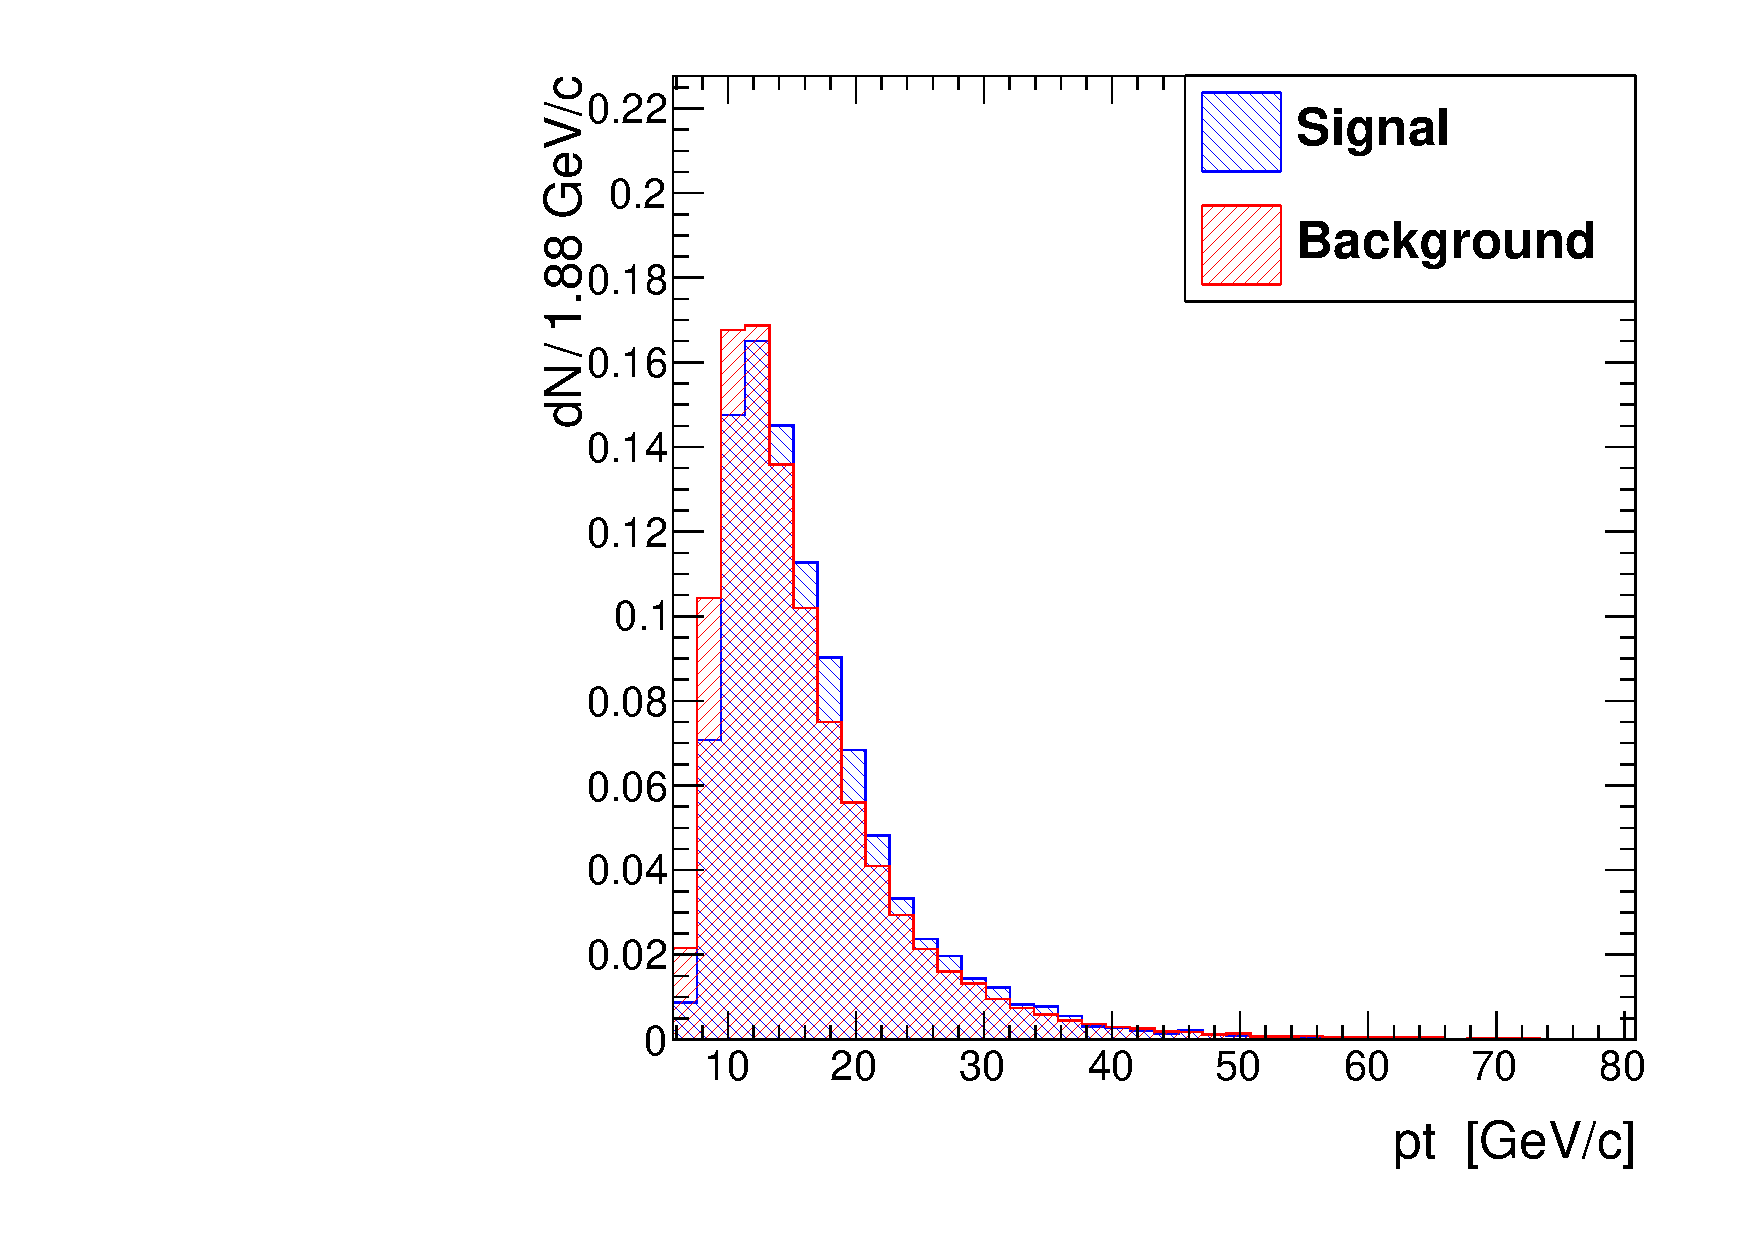
\includegraphics[width=\textwidth]{Figures/pt_barrel}
                \label{fig:ptBarrel}
        \end{subfigure}
        ~
        \begin{subfigure}[b]{0.2\textwidth}
                \centering
                % 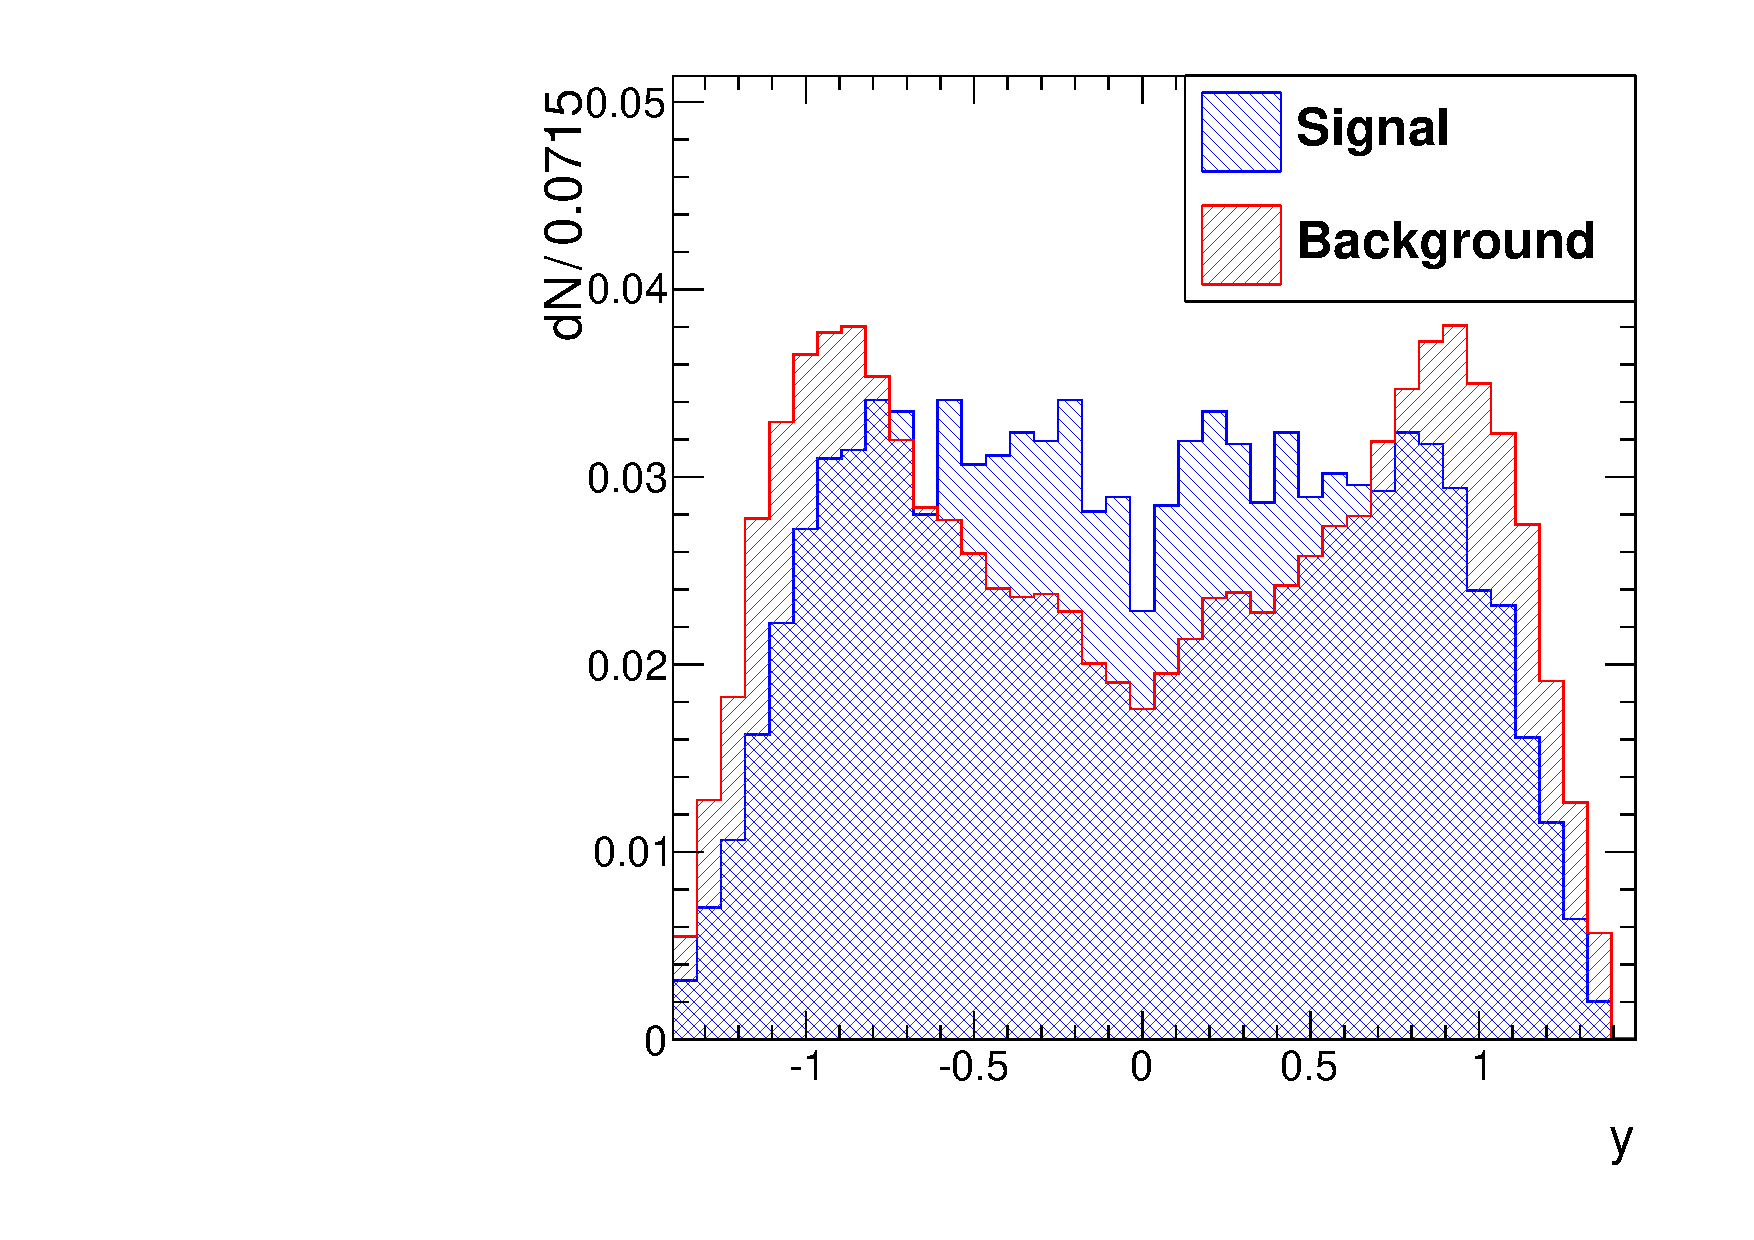
\includegraphics[width=\textwidth]{Figures/y_barrel}
                % \label{fig:yBarrel}
                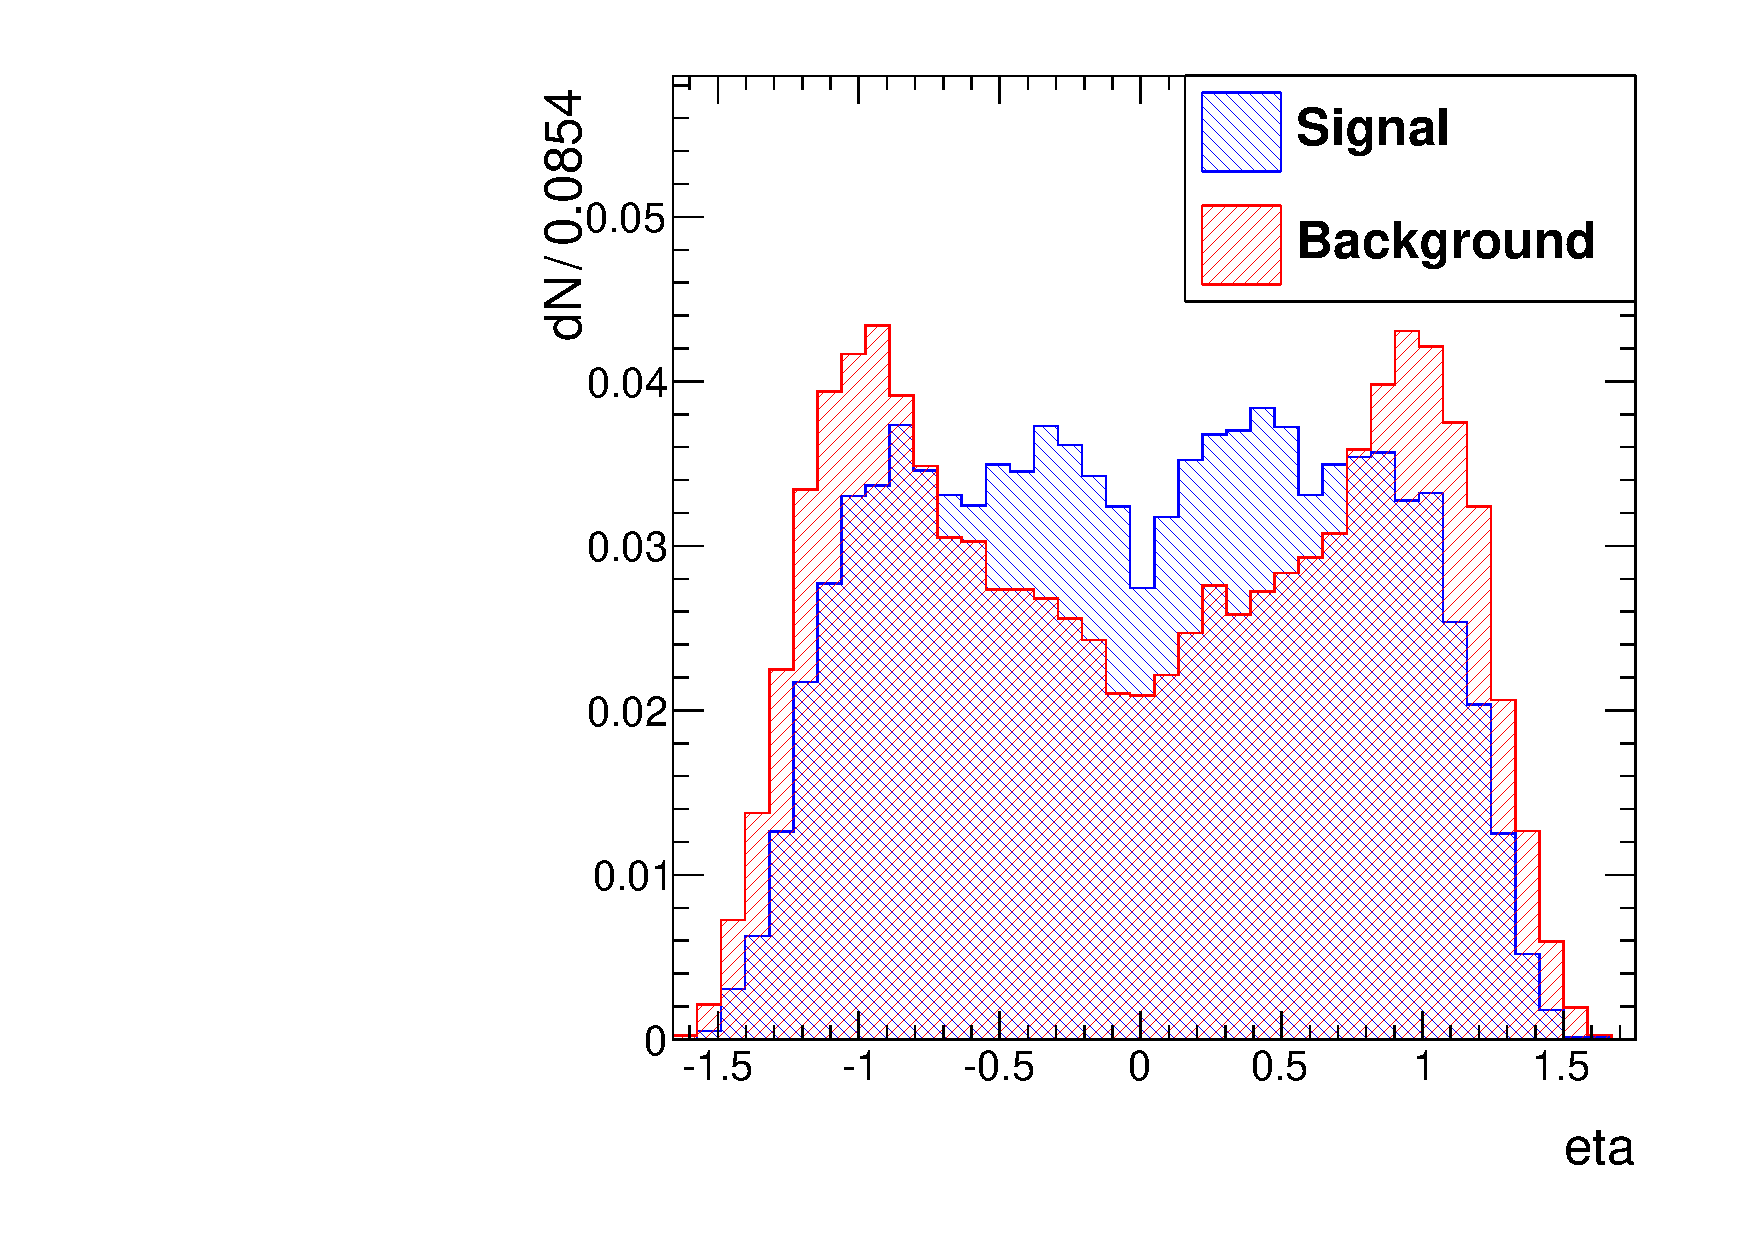
\includegraphics[width=\textwidth]{Figures/eta_barrel}
                \label{fig:etaBarrel}
        \end{subfigure}
        ~
        \begin{subfigure}[b]{0.2\textwidth}
                \centering
                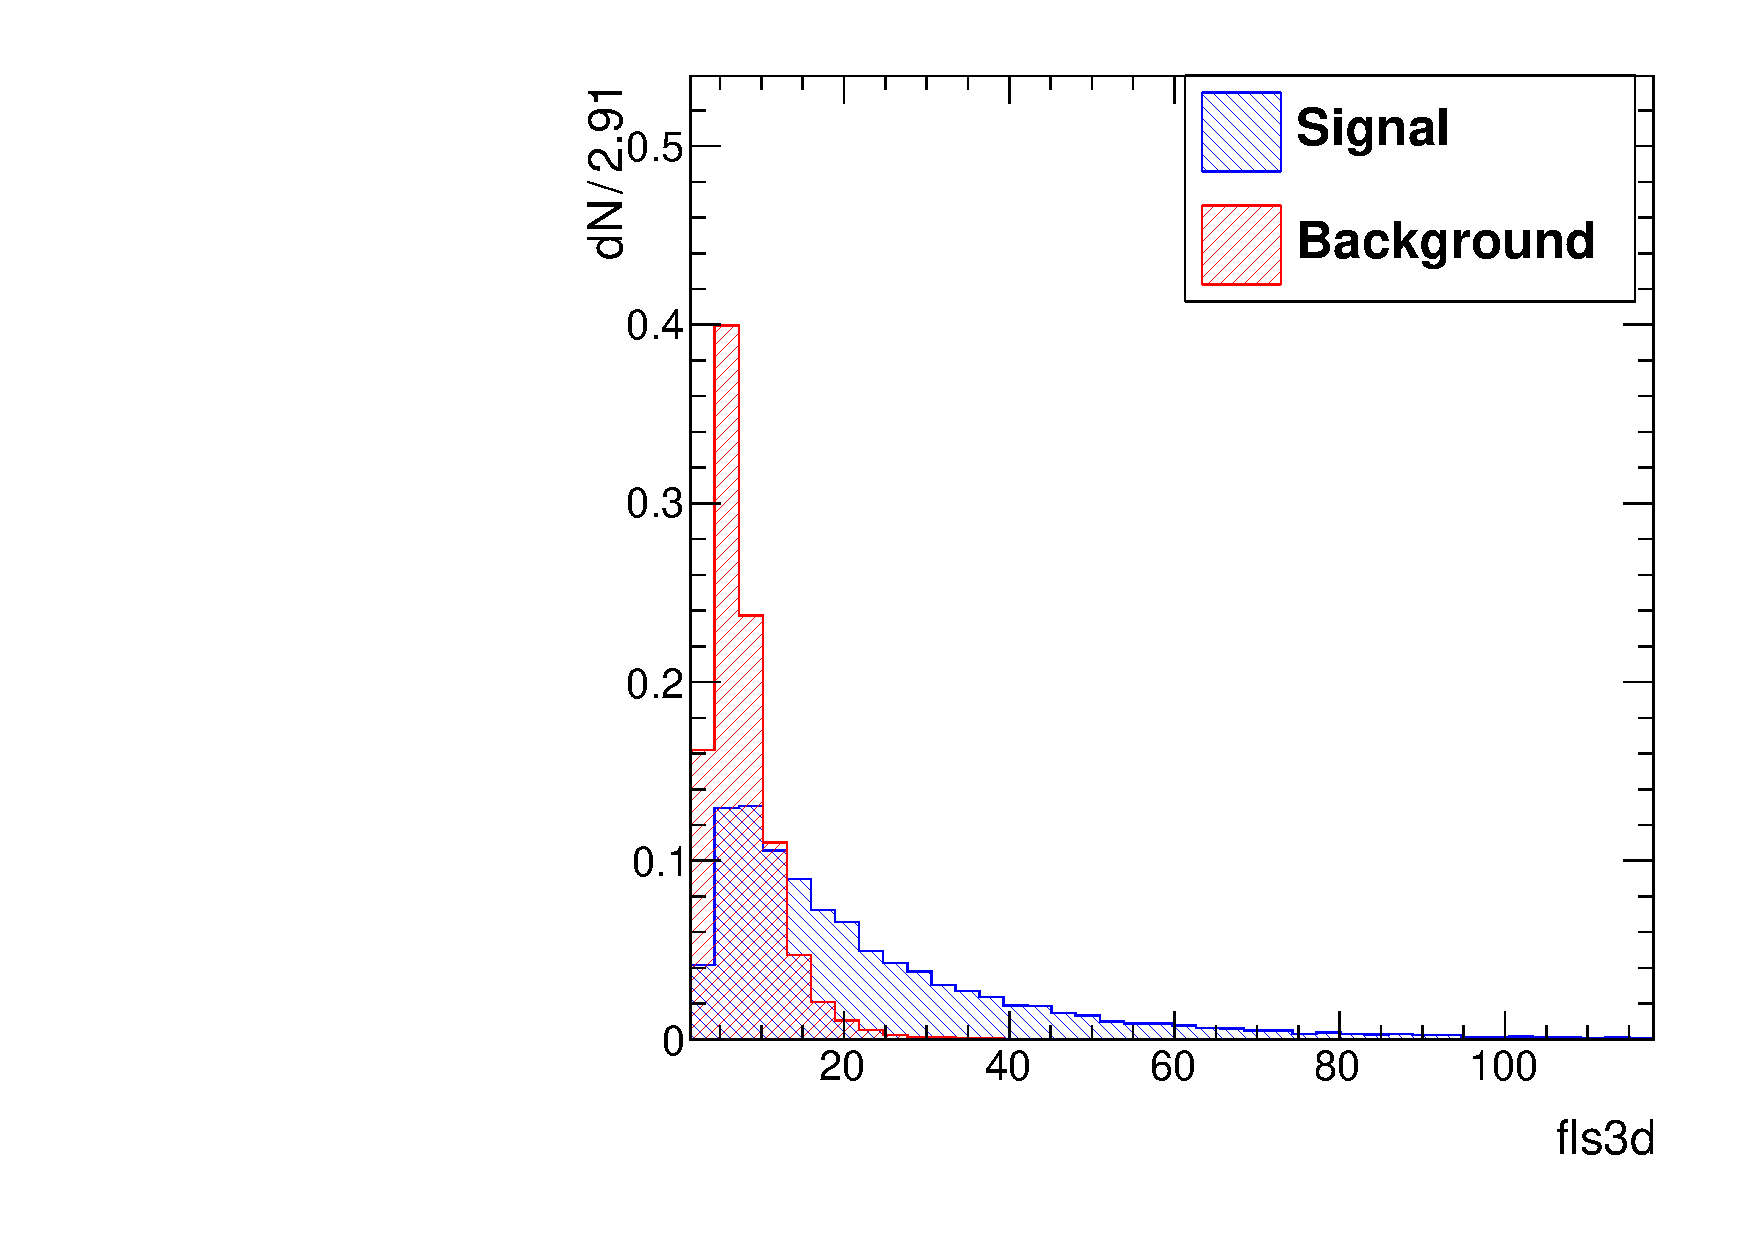
\includegraphics[width=\textwidth]{Figures/fls3d_barrel}
                \label{fig:fls3dBarrel}
        \end{subfigure}
        ~
        \begin{subfigure}[b]{0.2\textwidth}
                \centering
                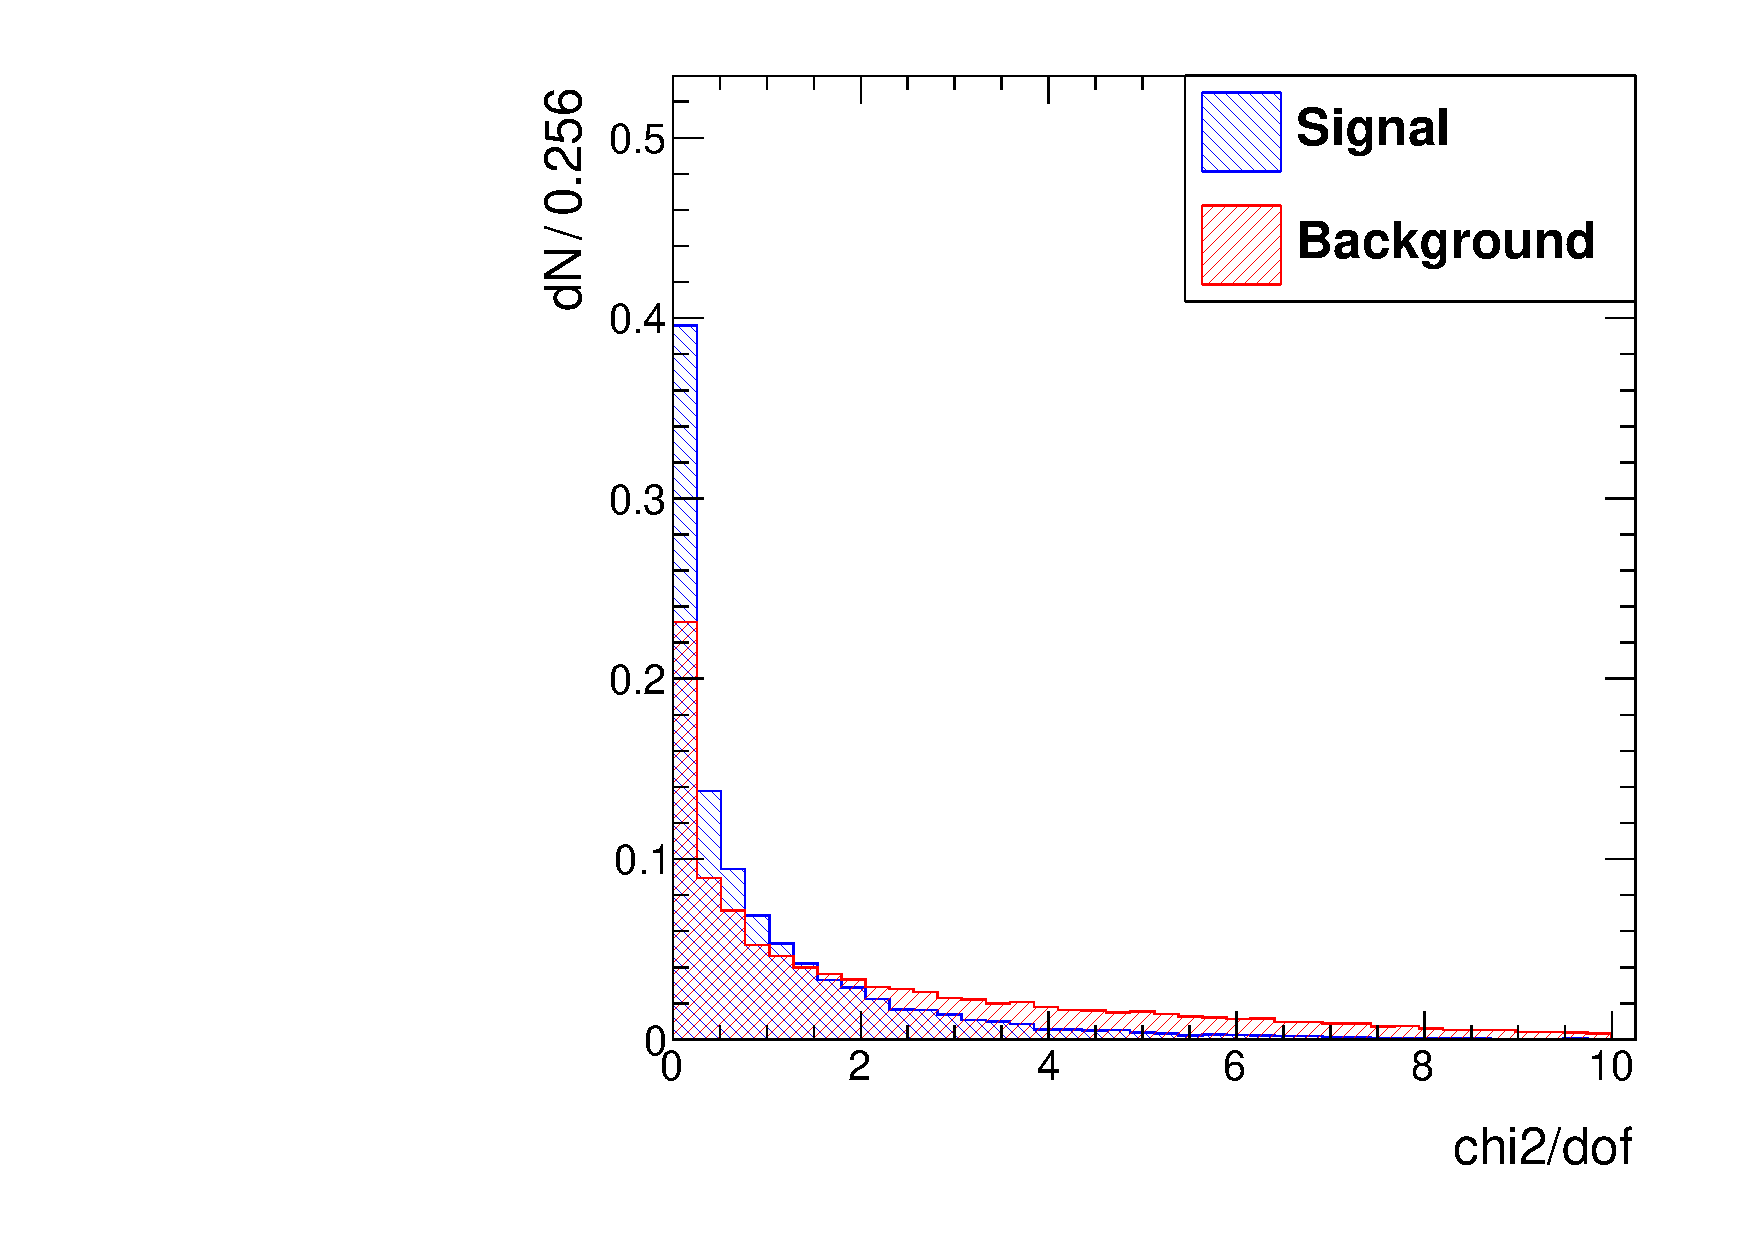
\includegraphics[width=\textwidth]{Figures/chi2dof_barrel}
                \label{fig:chi2dofBarrel}
        \end{subfigure}
        
        \begin{subfigure}[b]{0.2\textwidth}
                \centering
                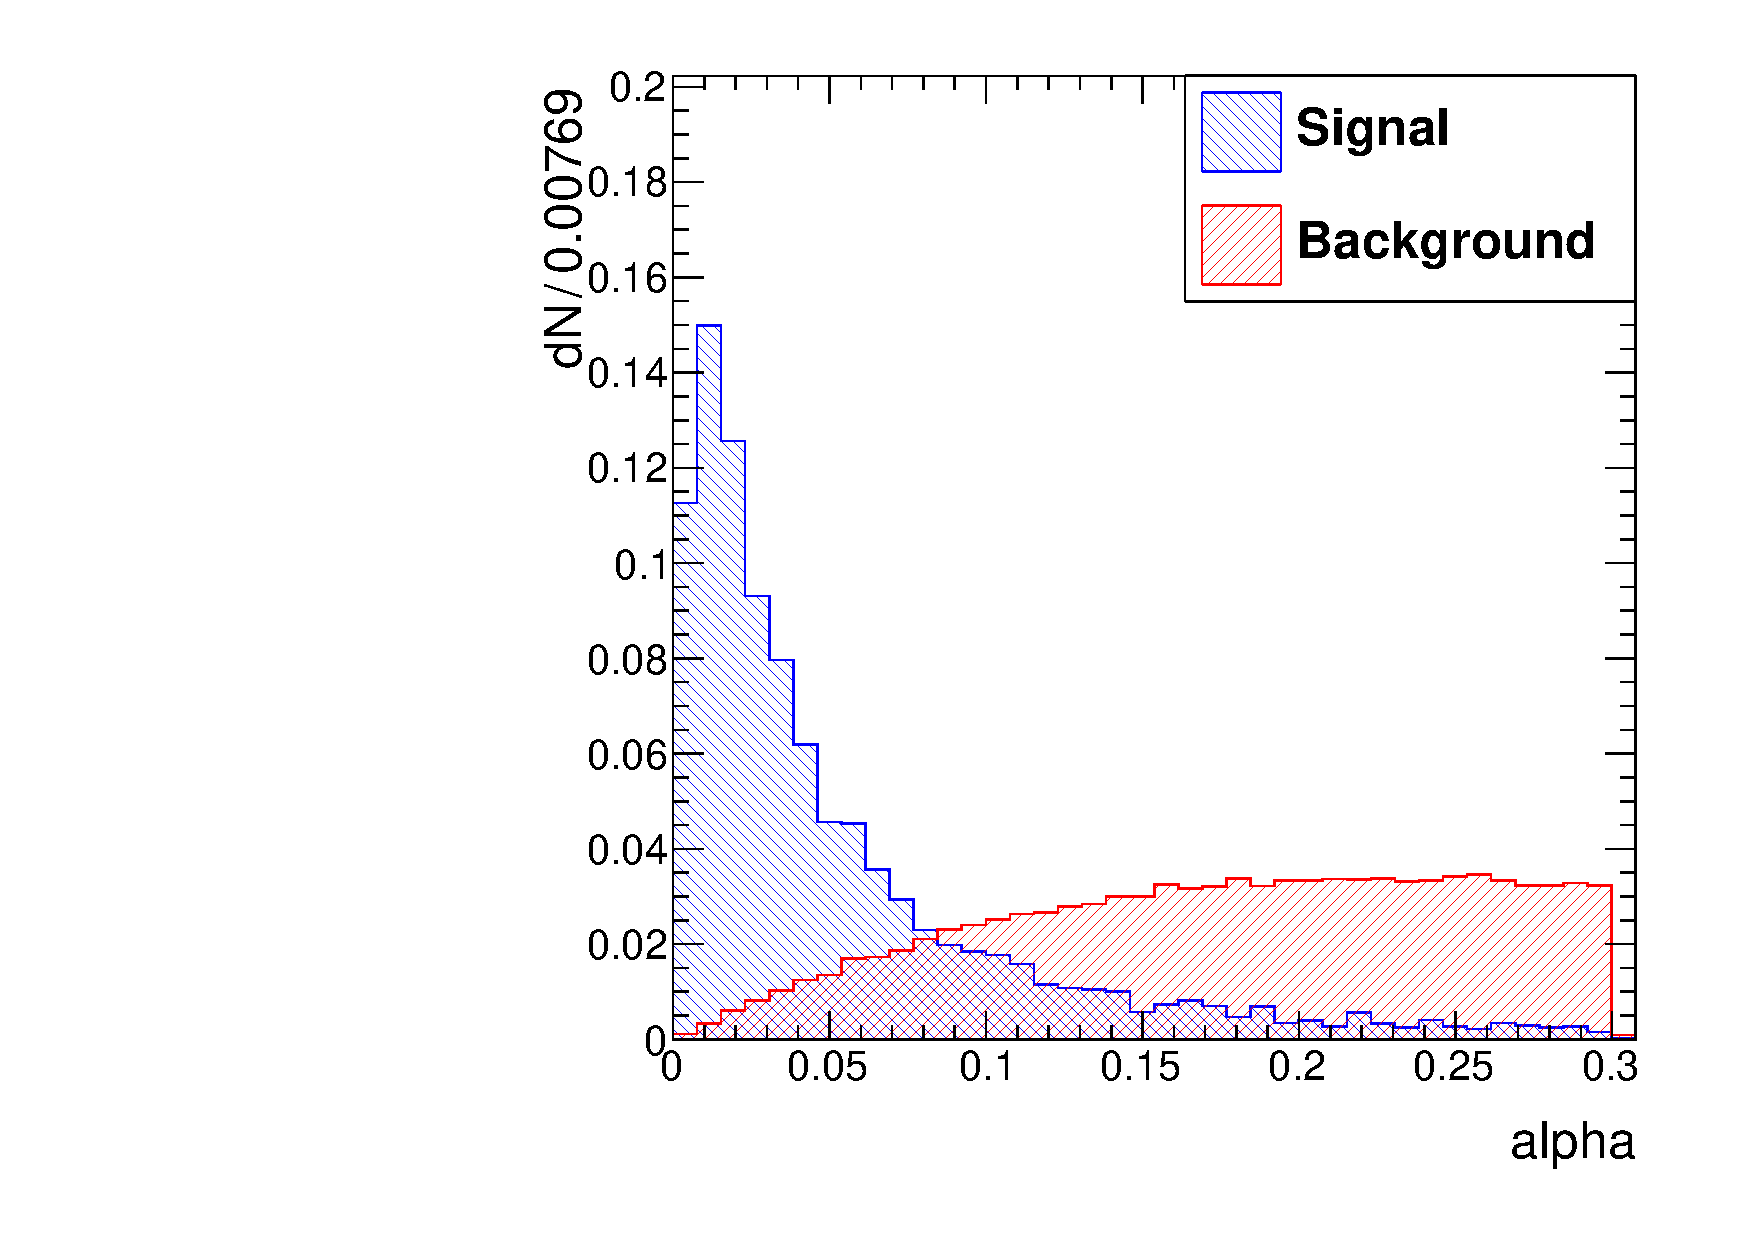
\includegraphics[width=\textwidth]{Figures/alpha_barrel}
                \label{fig:alphaBarrel}
        \end{subfigure}
        ~
        \begin{subfigure}[b]{0.2\textwidth}
                \centering
                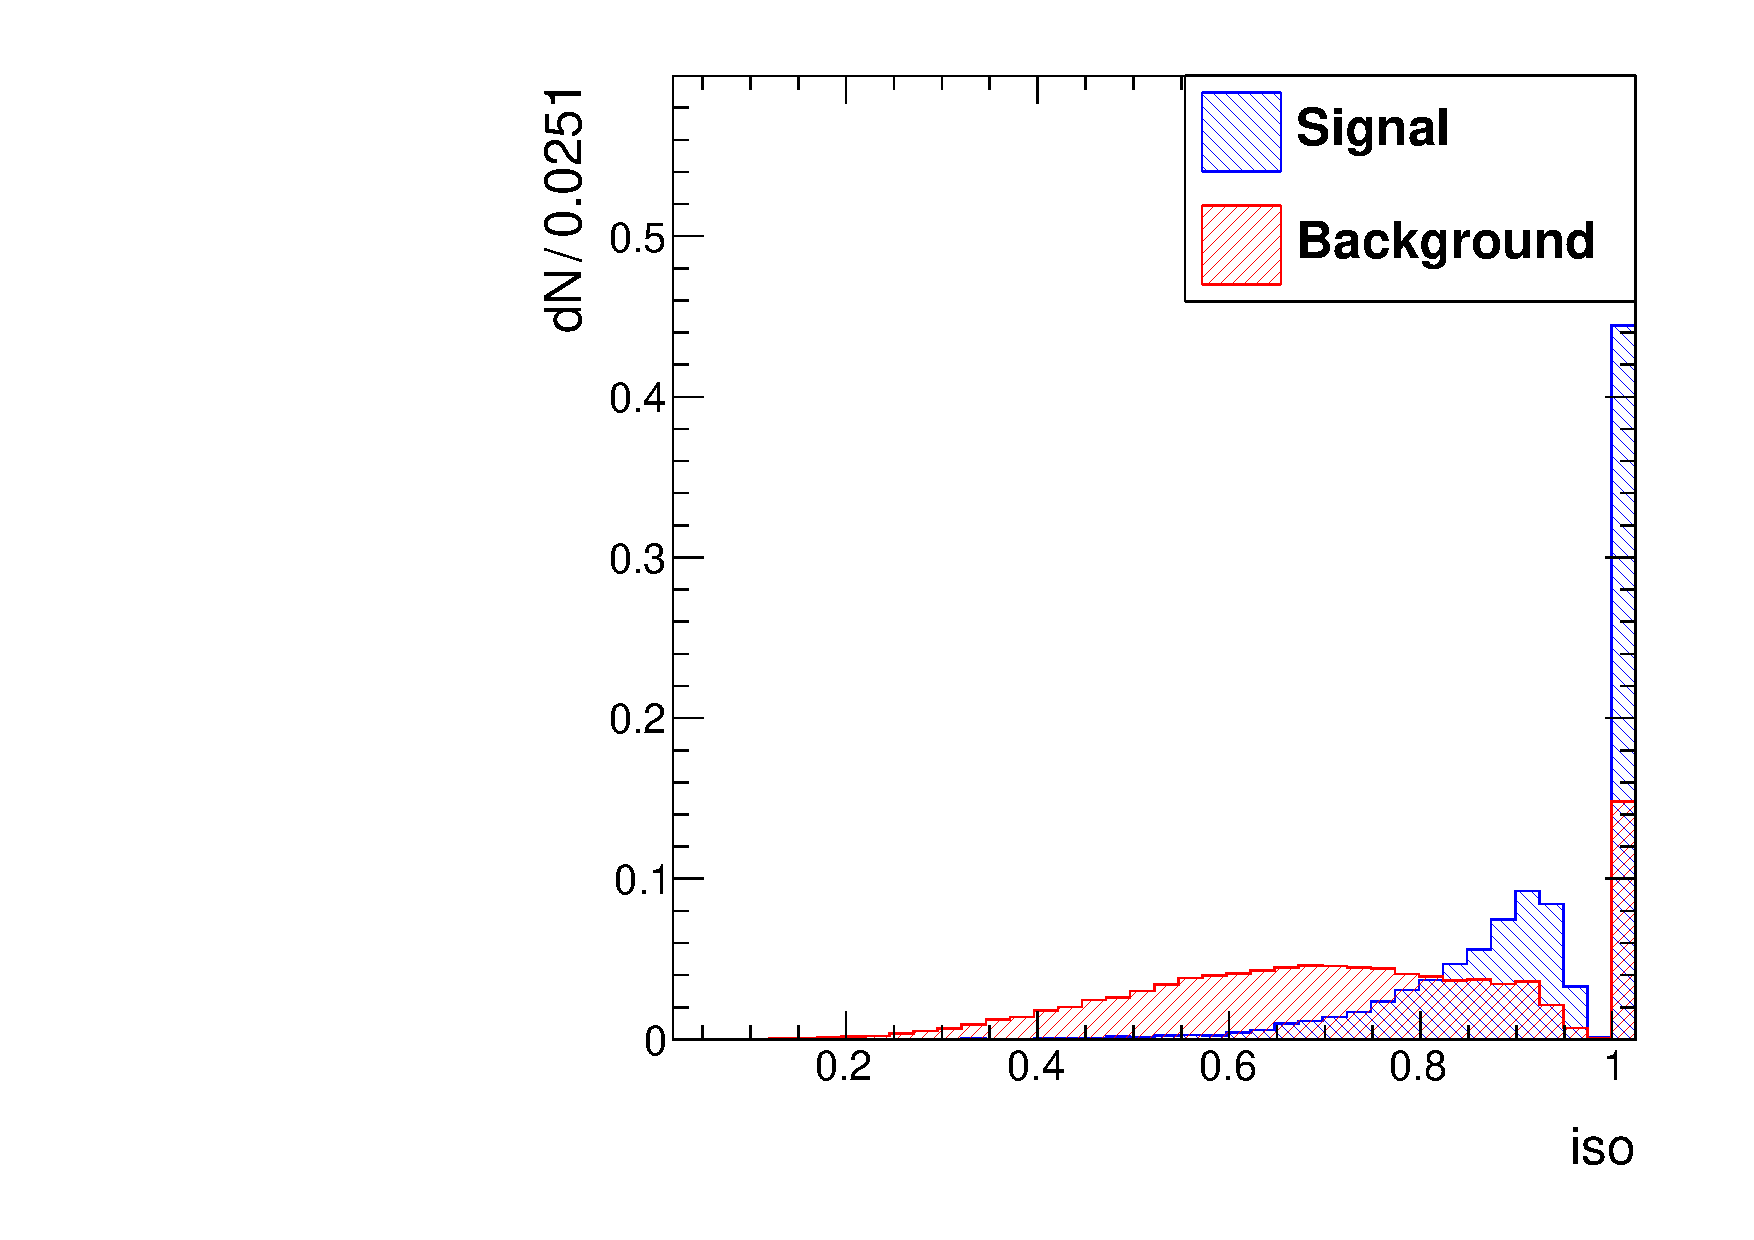
\includegraphics[width=\textwidth]{Figures/iso_barrel}
                \label{fig:isoBarrel}
        \end{subfigure}
        ~
        \begin{subfigure}[b]{0.2\textwidth}
                \centering
                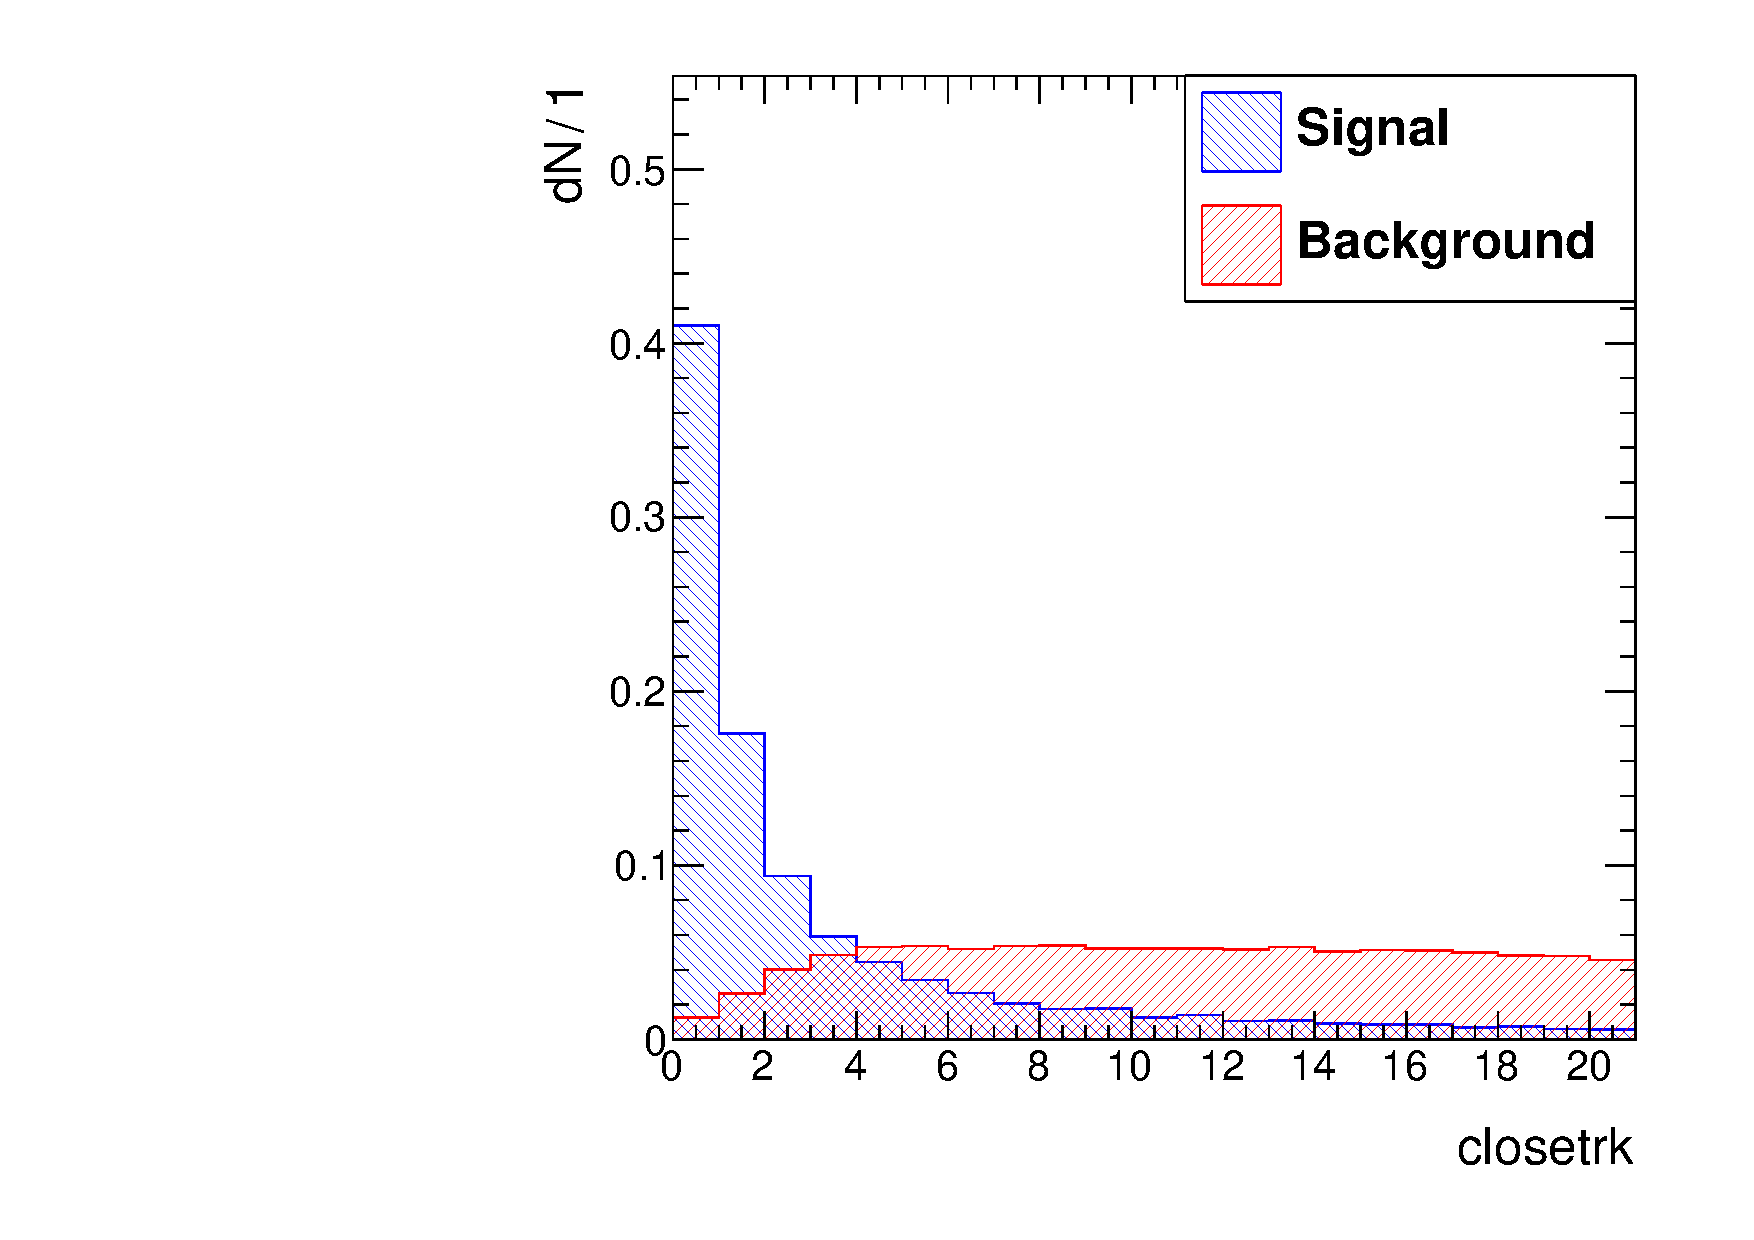
\includegraphics[width=\textwidth]{Figures/closetrk_barrel}
                \label{fig:closetrkBarrel}
        \end{subfigure}
        ~
        \begin{subfigure}[b]{0.2\textwidth}
                \centering
                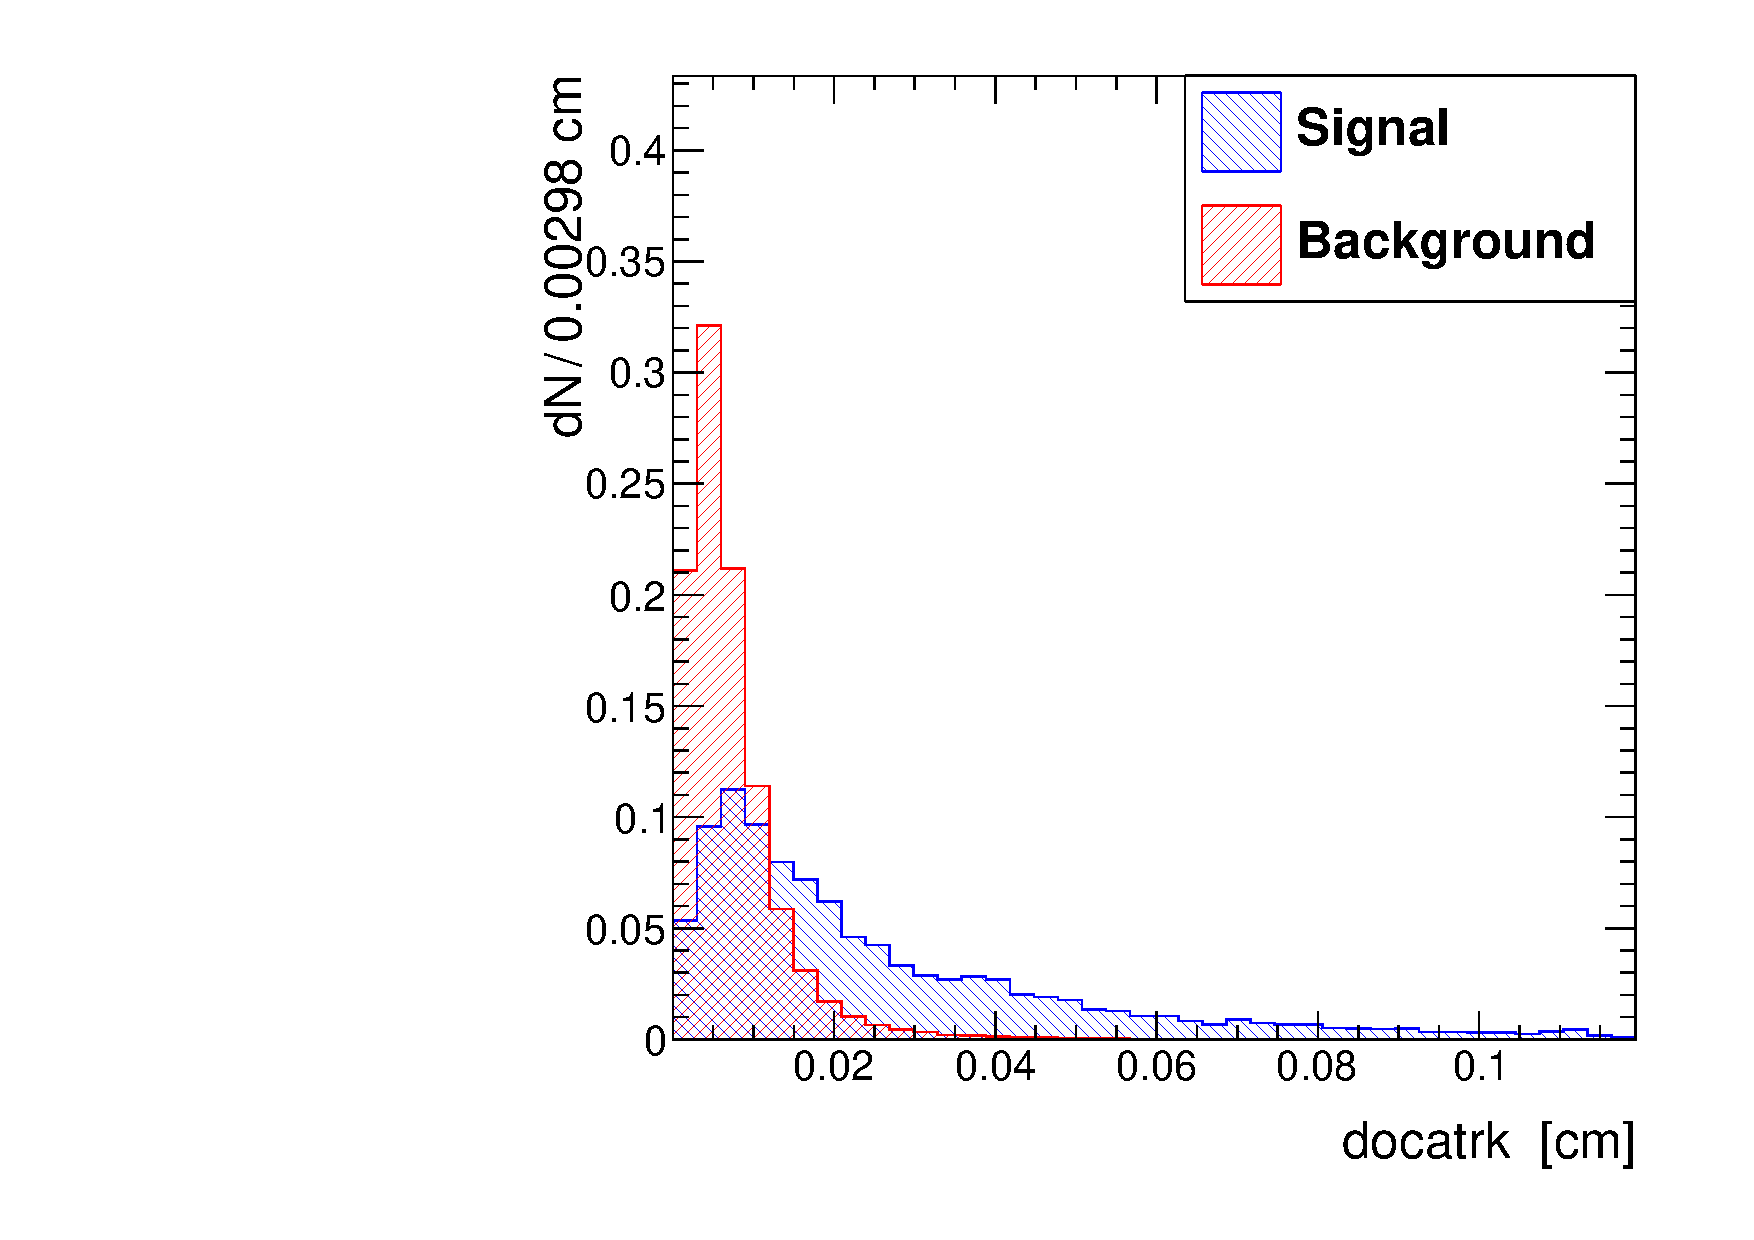
\includegraphics[width=\textwidth]{Figures/docatrk_barrel}
                \label{fig:docatrkBarrel}
        \end{subfigure}

        \begin{subfigure}[b]{0.2\textwidth}
                \centering
                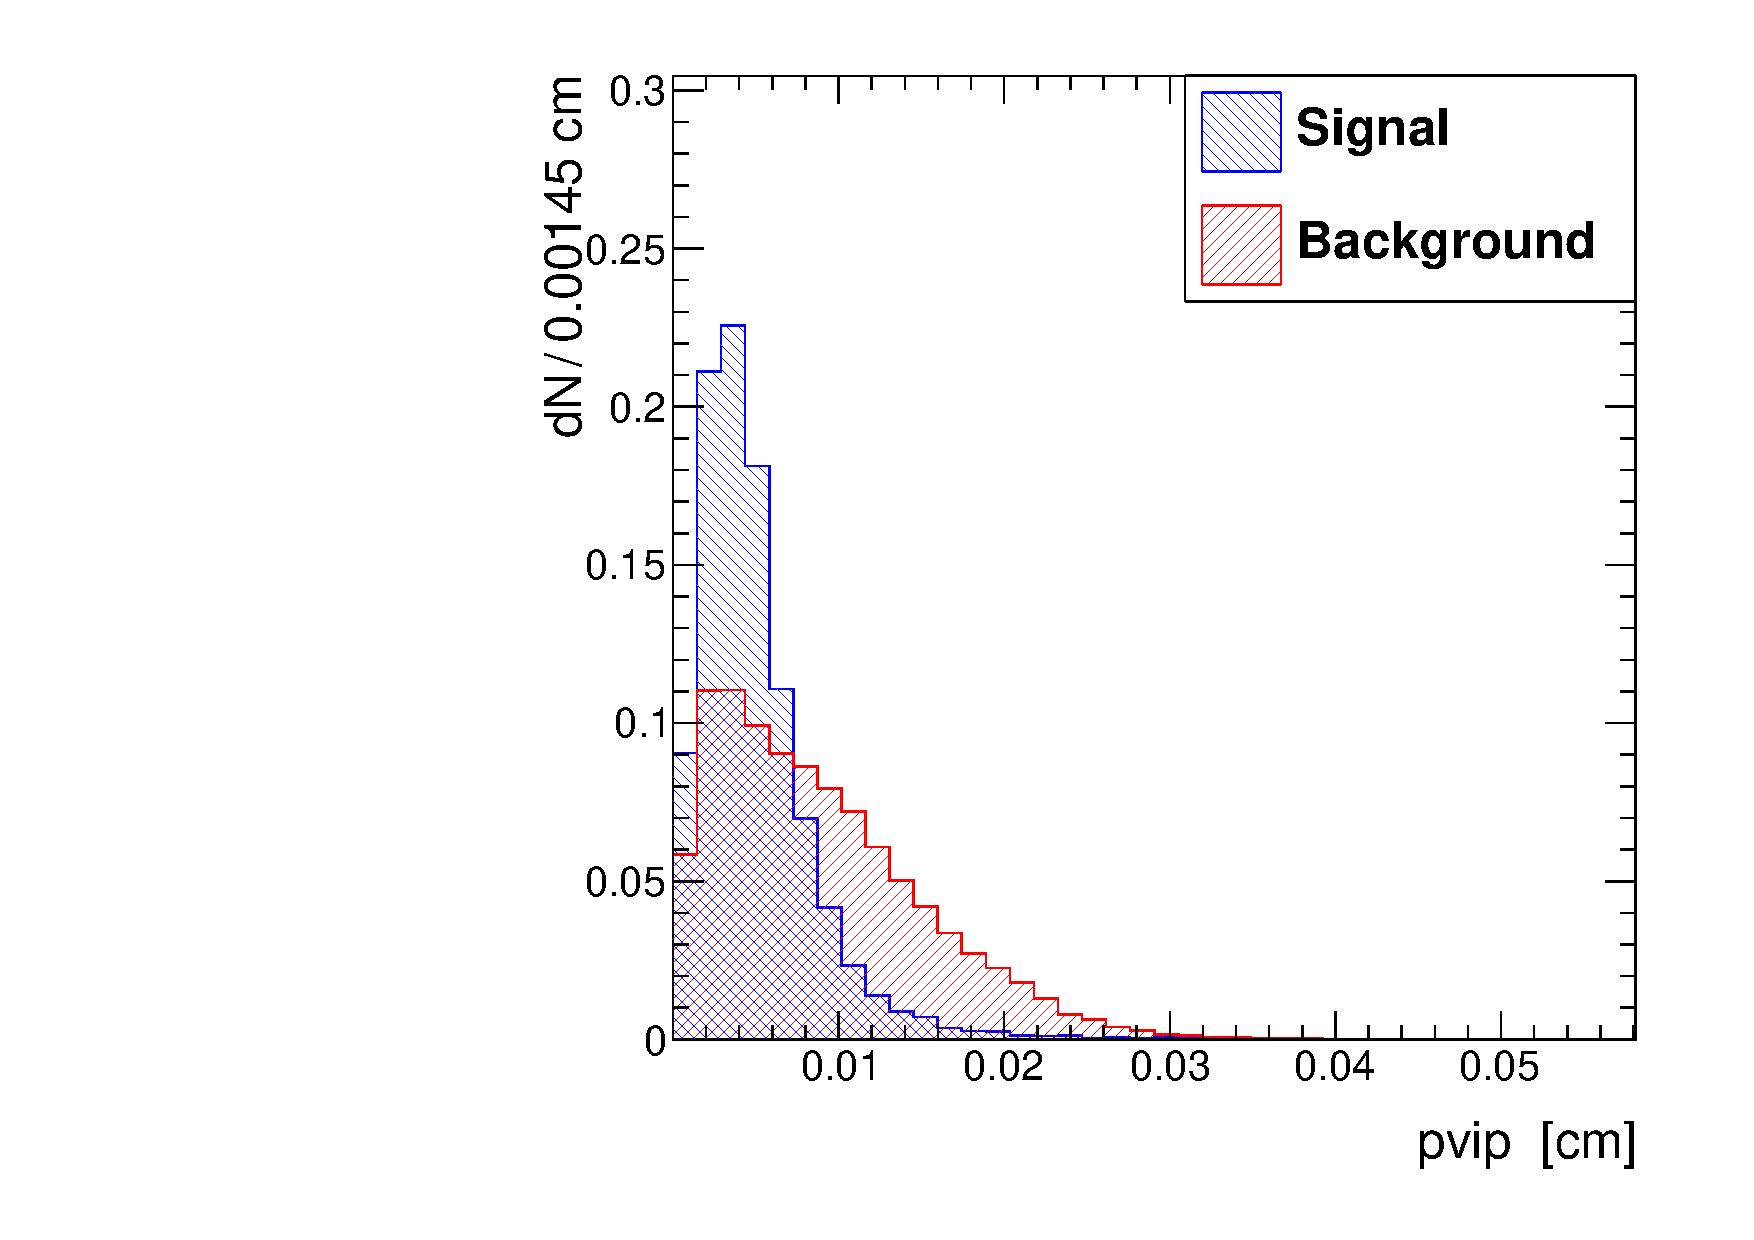
\includegraphics[width=\textwidth]{Figures/pvip_barrel}
                \label{fig:pvipBarrel}
        \end{subfigure}
        ~
        \begin{subfigure}[b]{0.2\textwidth}
                \centering
                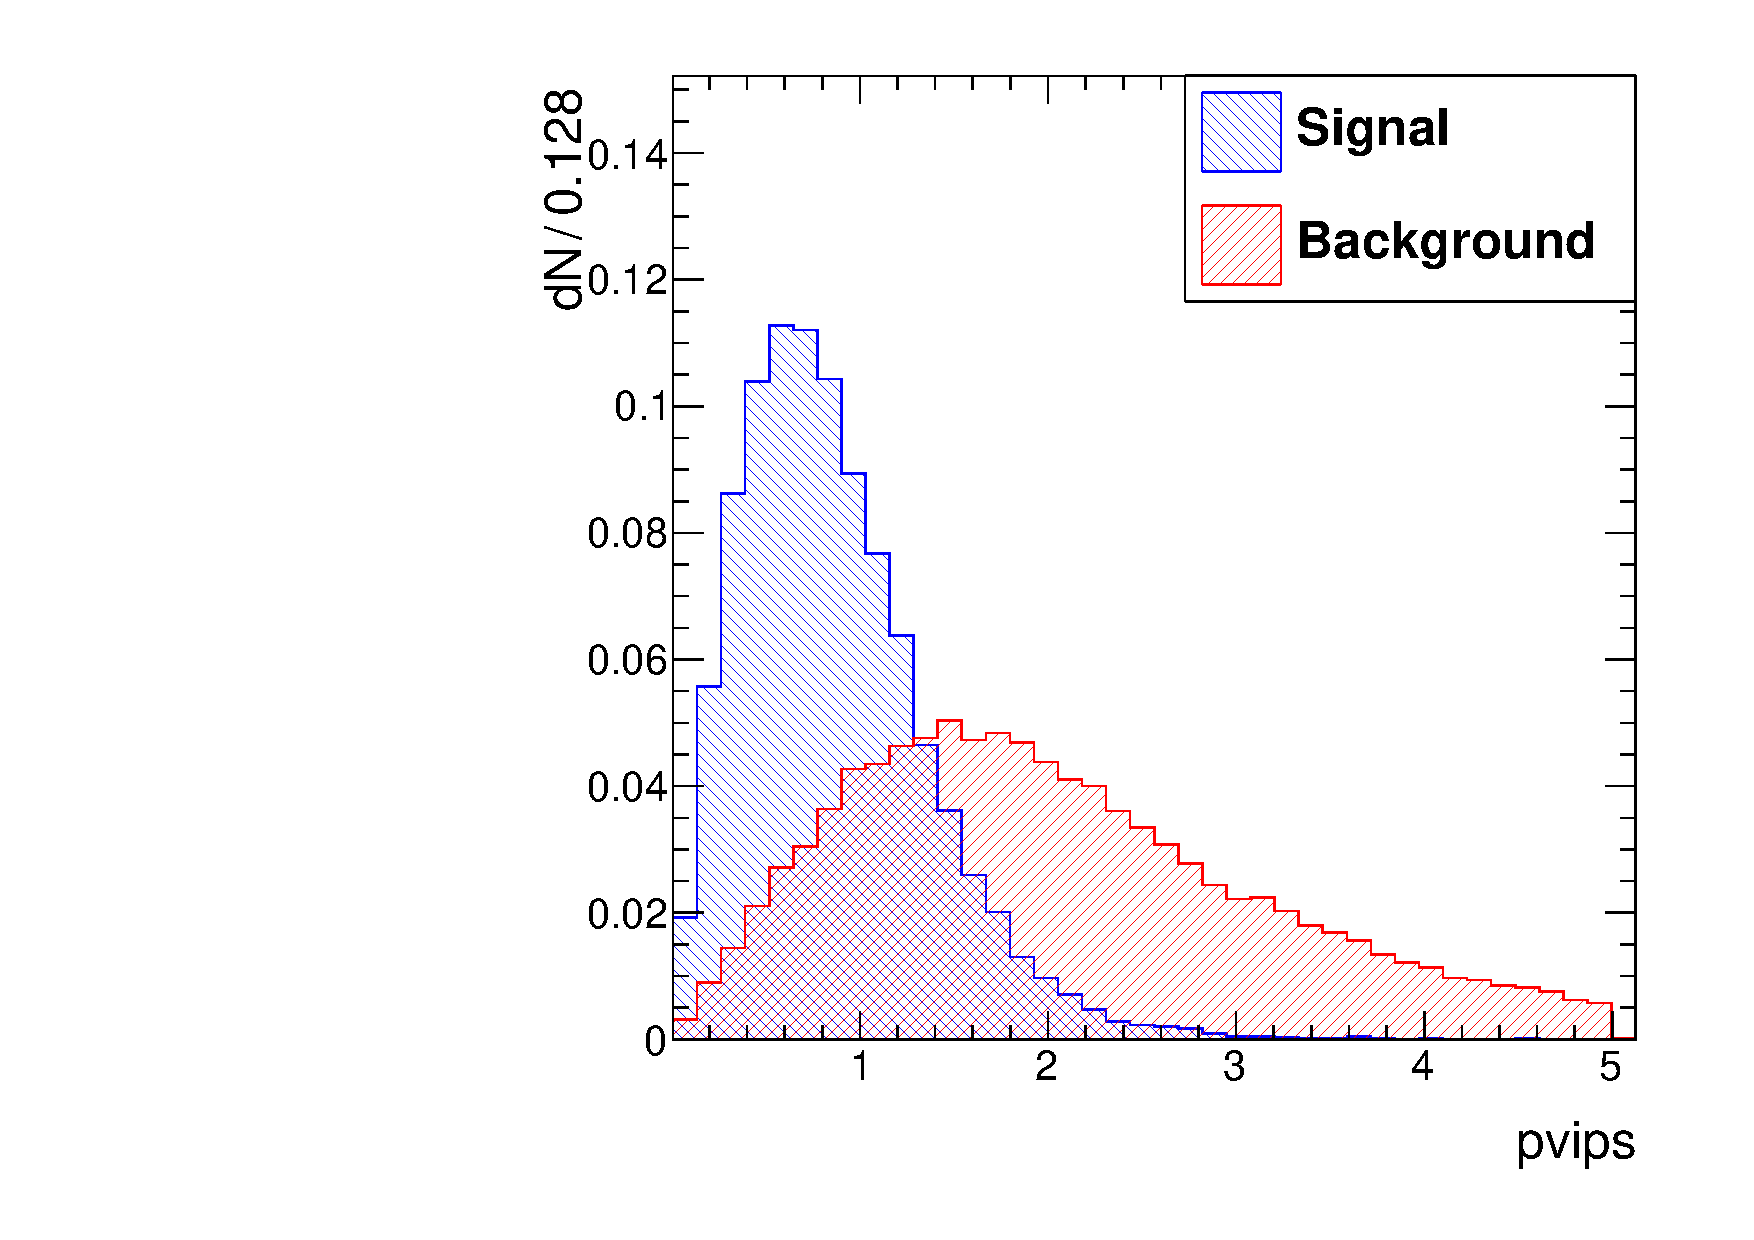
\includegraphics[width=\textwidth]{Figures/pvips_barrel}
                \label{fig:pvipsBarrel}
        \end{subfigure}
        ~
        \begin{subfigure}[b]{0.2\textwidth}
                \centering
                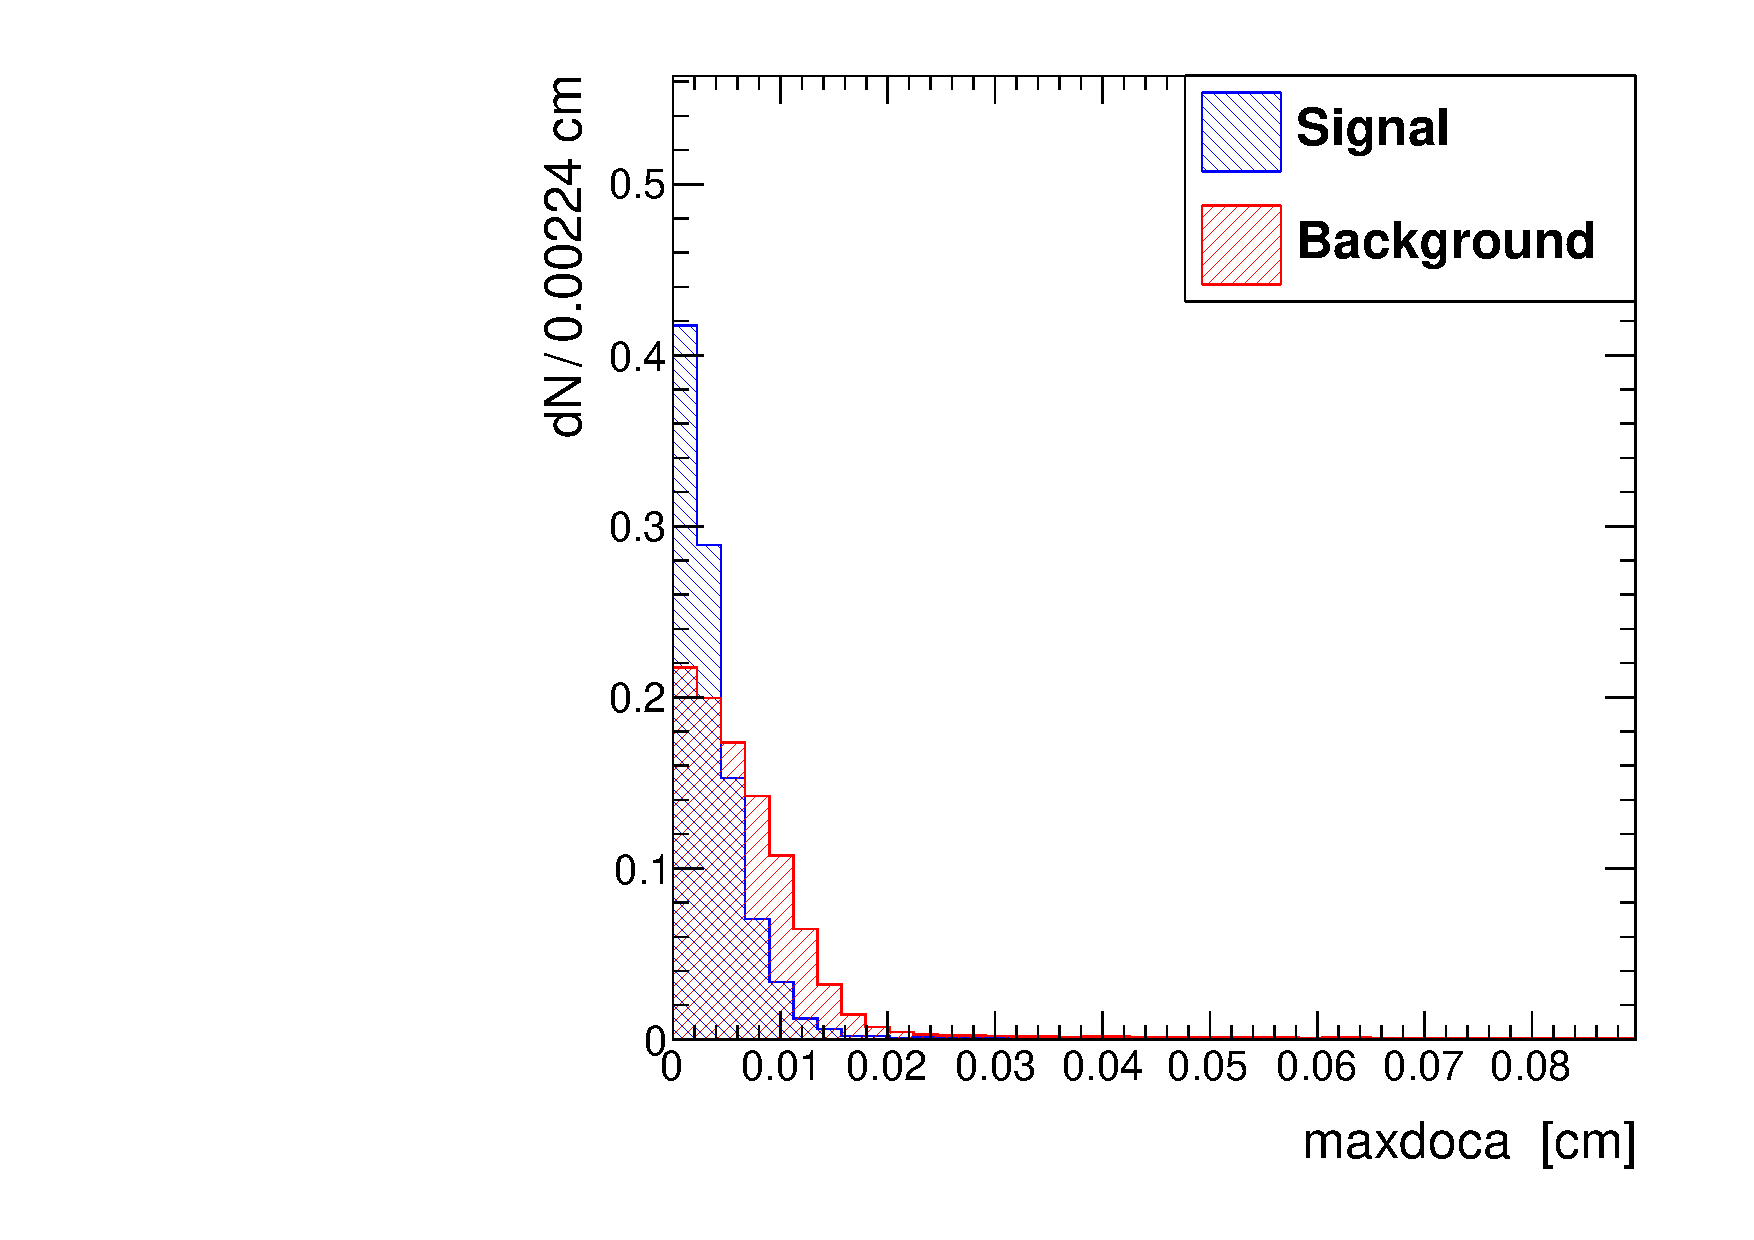
\includegraphics[width=\textwidth]{Figures/maxdoca_barrel}
                \label{fig:maxdocaBarrel}
        \end{subfigure}
        \caption{Standard TMVA plot of the input variables for the barrel BDT for signal (blue) and background (red). The background is extracted from data dimuon sidebands.}
        \label{fig:TMVAPlotsBarrel}
\end{sidewaysfigure}

\begin{sidewaysfigure}
        \centering
        \begin{subfigure}[b]{0.2\textwidth}
                \centering
                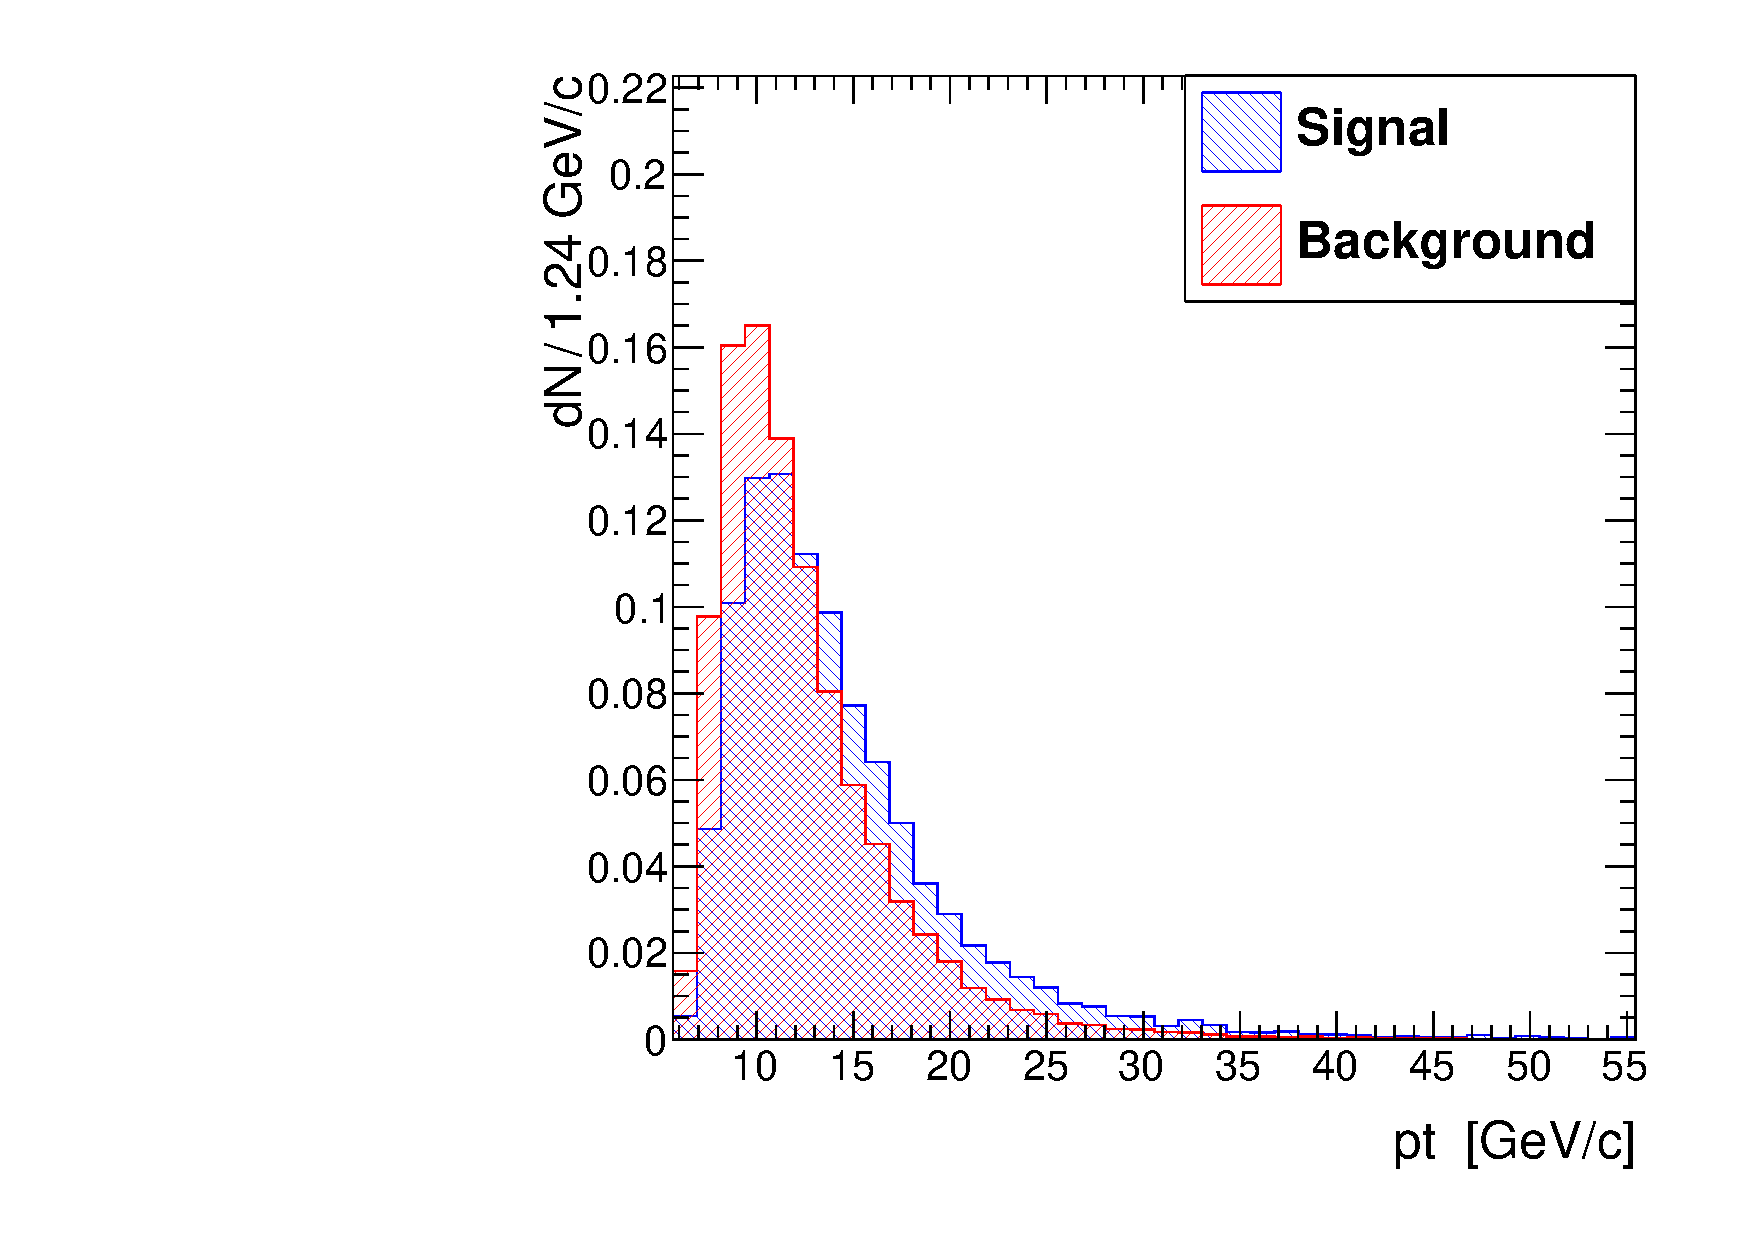
\includegraphics[width=\textwidth]{Figures/pt_endcaps}
                \label{fig:ptEndcaps}
        \end{subfigure}
        ~
        \begin{subfigure}[b]{0.2\textwidth}
                \centering
                % 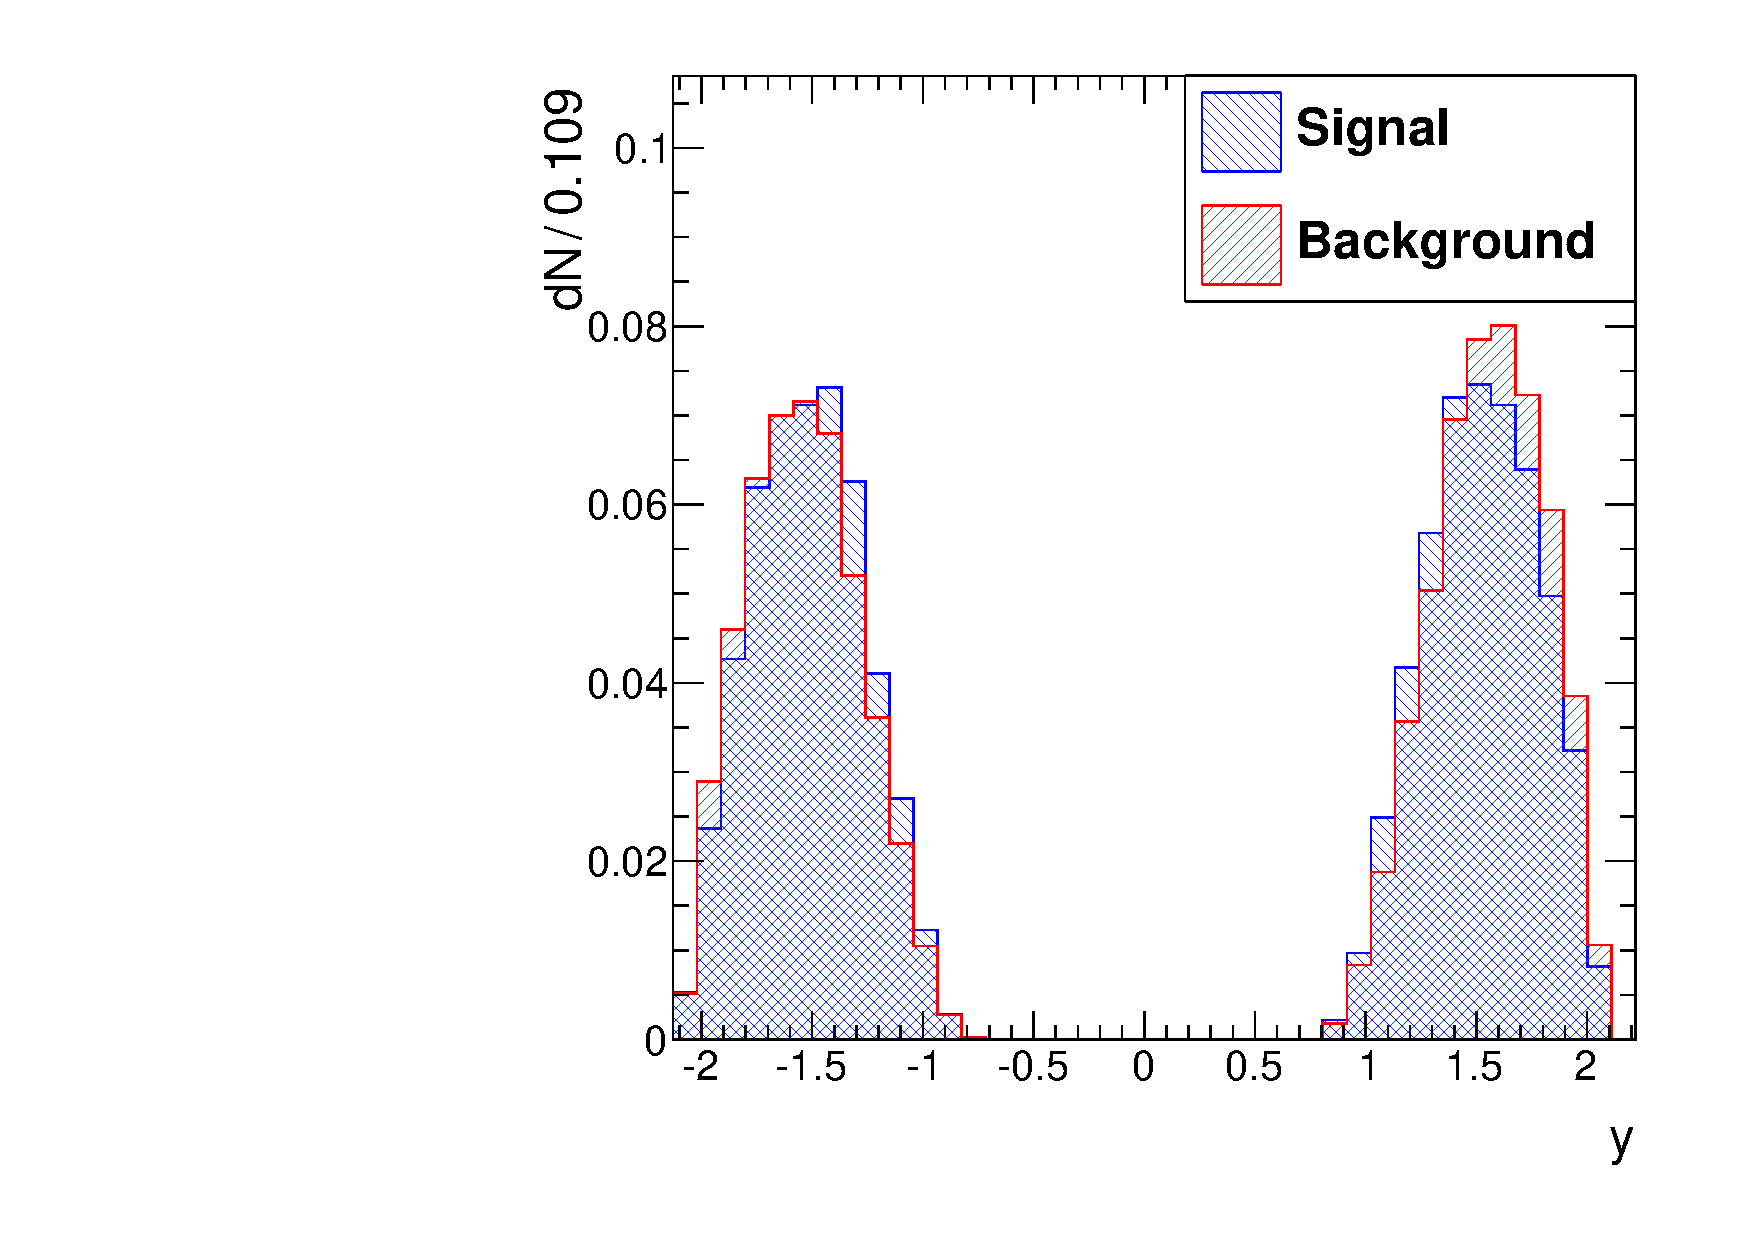
\includegraphics[width=\textwidth]{Figures/y_endcaps}
                % \label{fig:yEndcaps}
	            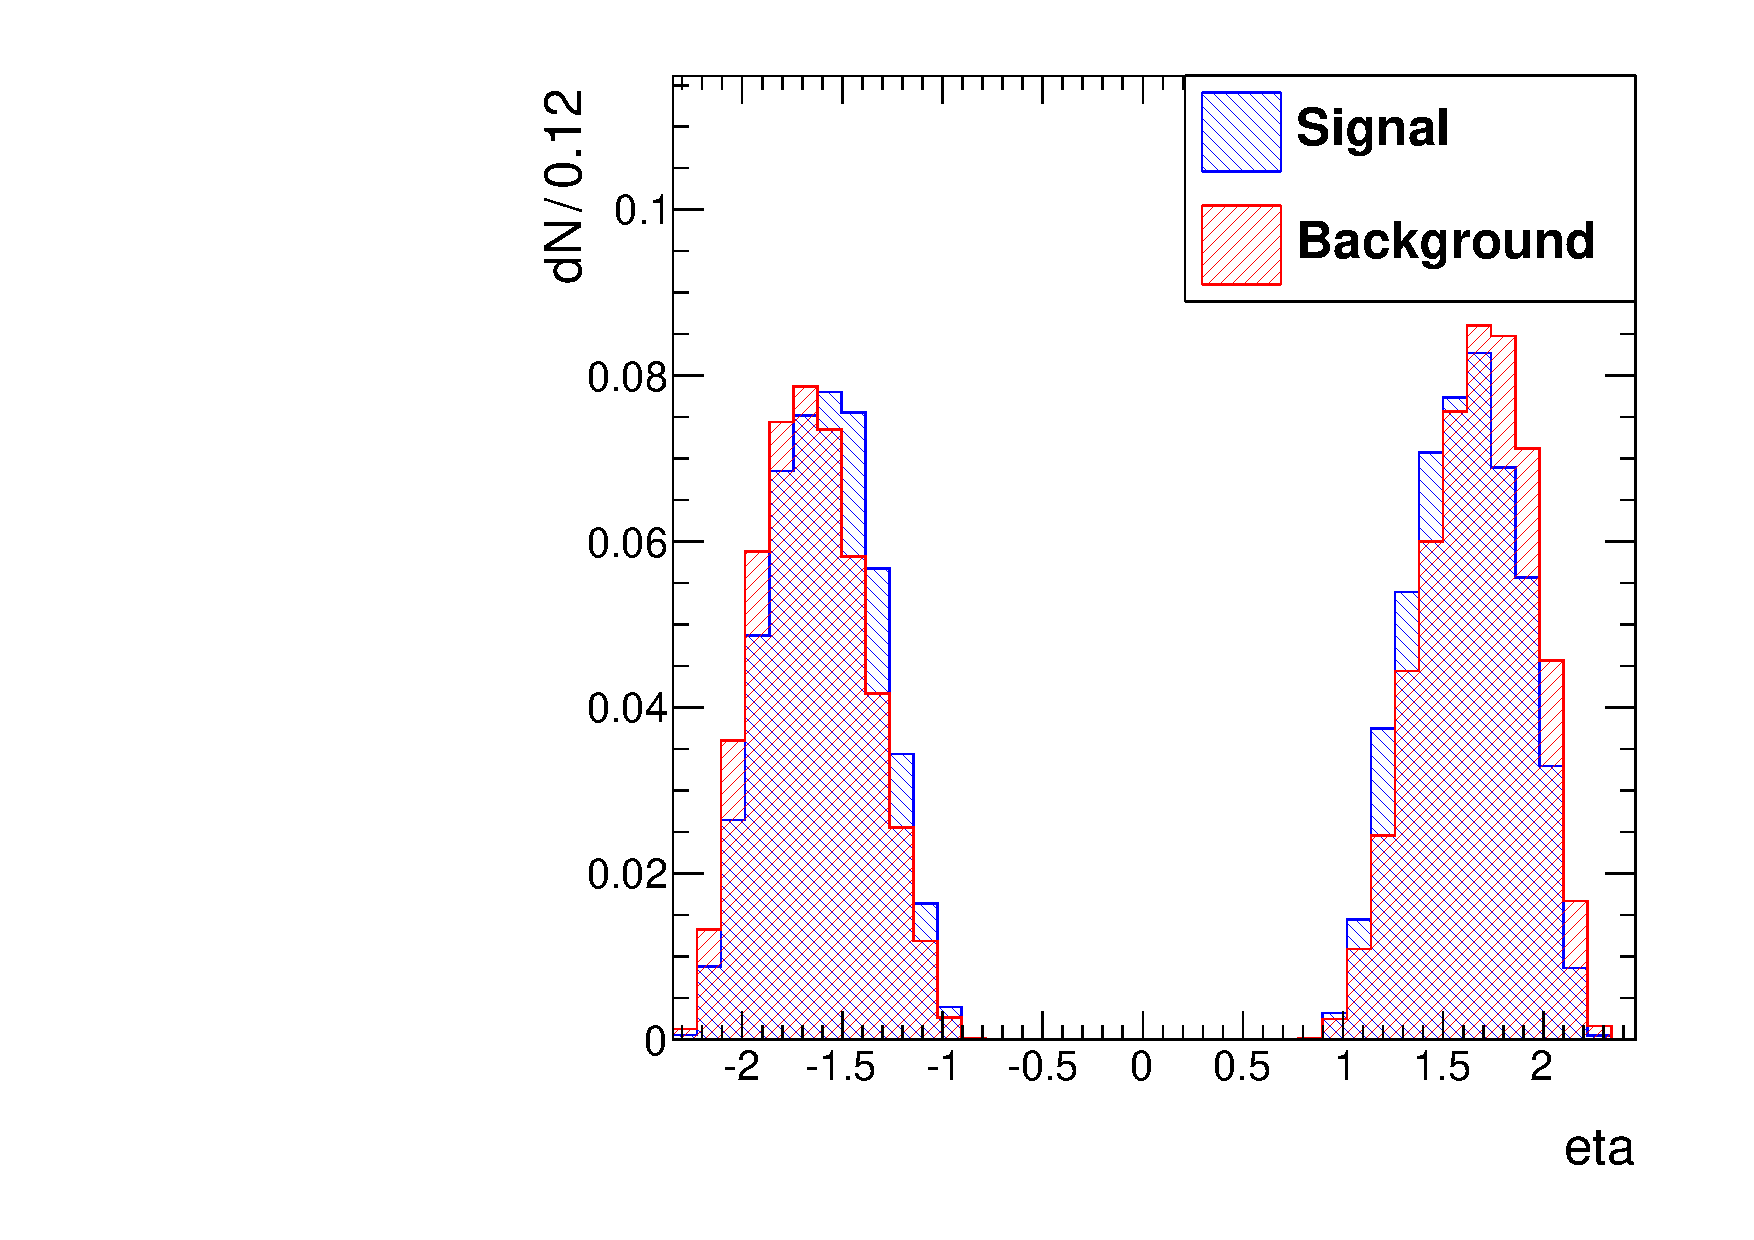
\includegraphics[width=\textwidth]{Figures/eta_endcaps}
                \label{fig:etaEndcaps}
        \end{subfigure}
        ~
        \begin{subfigure}[b]{0.2\textwidth}
                \centering
                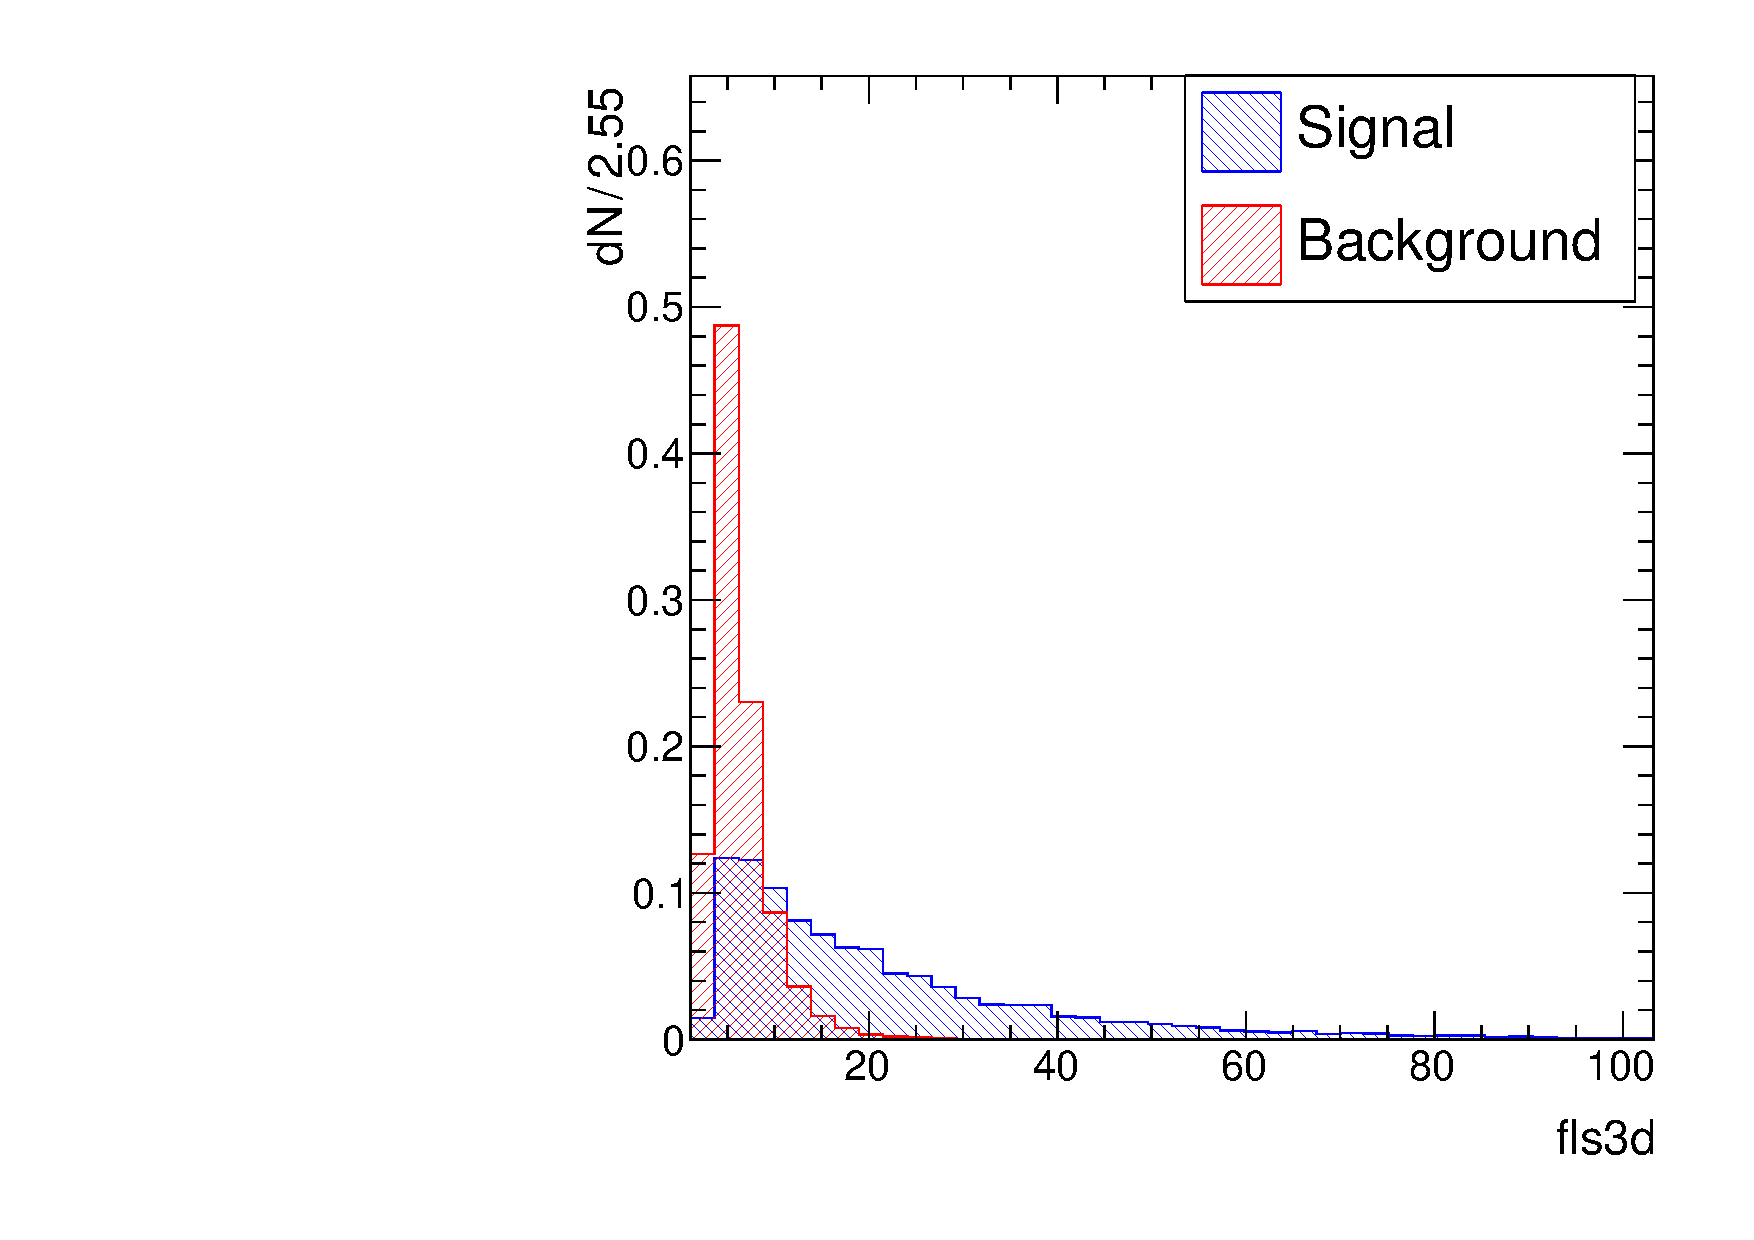
\includegraphics[width=\textwidth]{Figures/fls3d_endcaps}
                \label{fig:fls3dEndcaps}
        \end{subfigure}
        ~
        \begin{subfigure}[b]{0.2\textwidth}
                \centering
                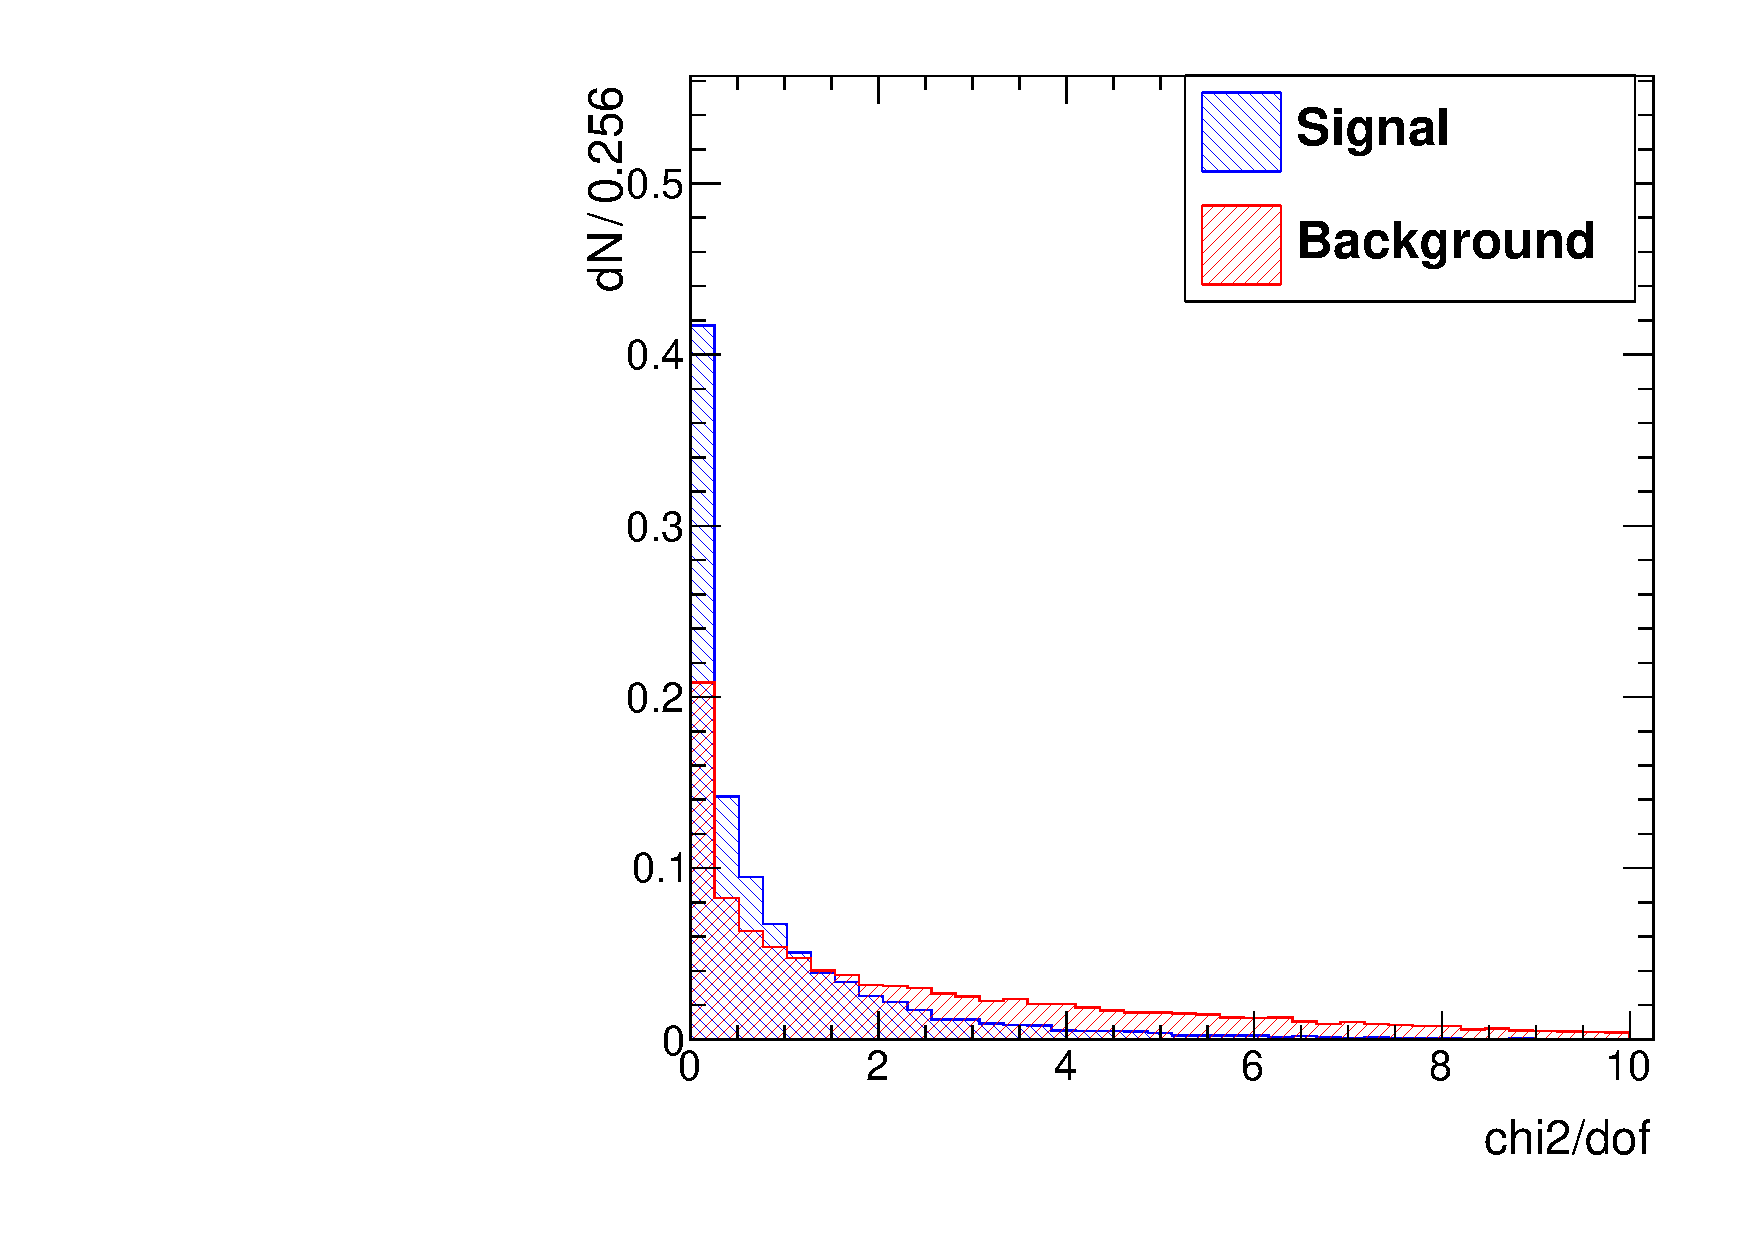
\includegraphics[width=\textwidth]{Figures/chi2dof_endcaps}
                \label{fig:chi2dofEndcaps}
        \end{subfigure}
        
        \begin{subfigure}[b]{0.2\textwidth}
                \centering
                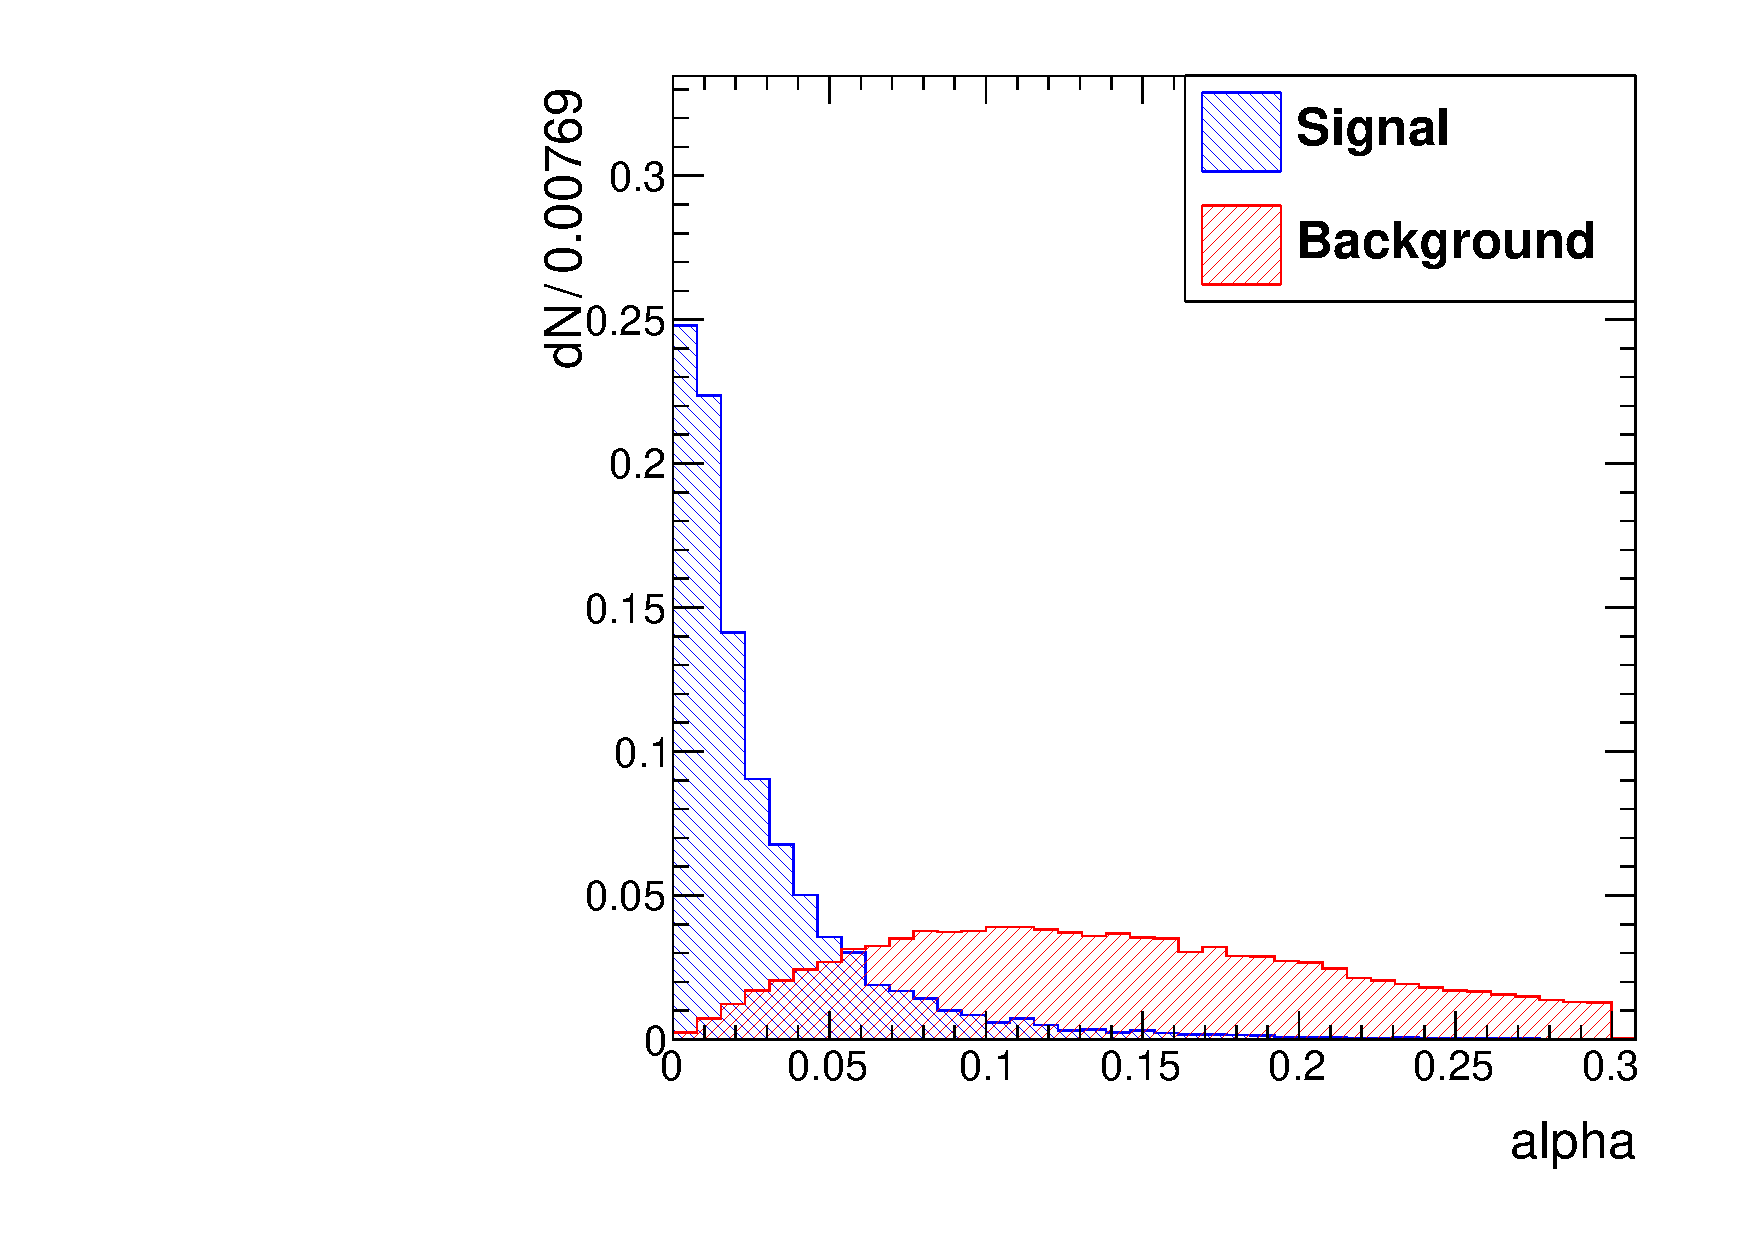
\includegraphics[width=\textwidth]{Figures/alpha_endcaps}
                \label{fig:alphaEndcaps}
        \end{subfigure}
        ~
        \begin{subfigure}[b]{0.2\textwidth}
                \centering
                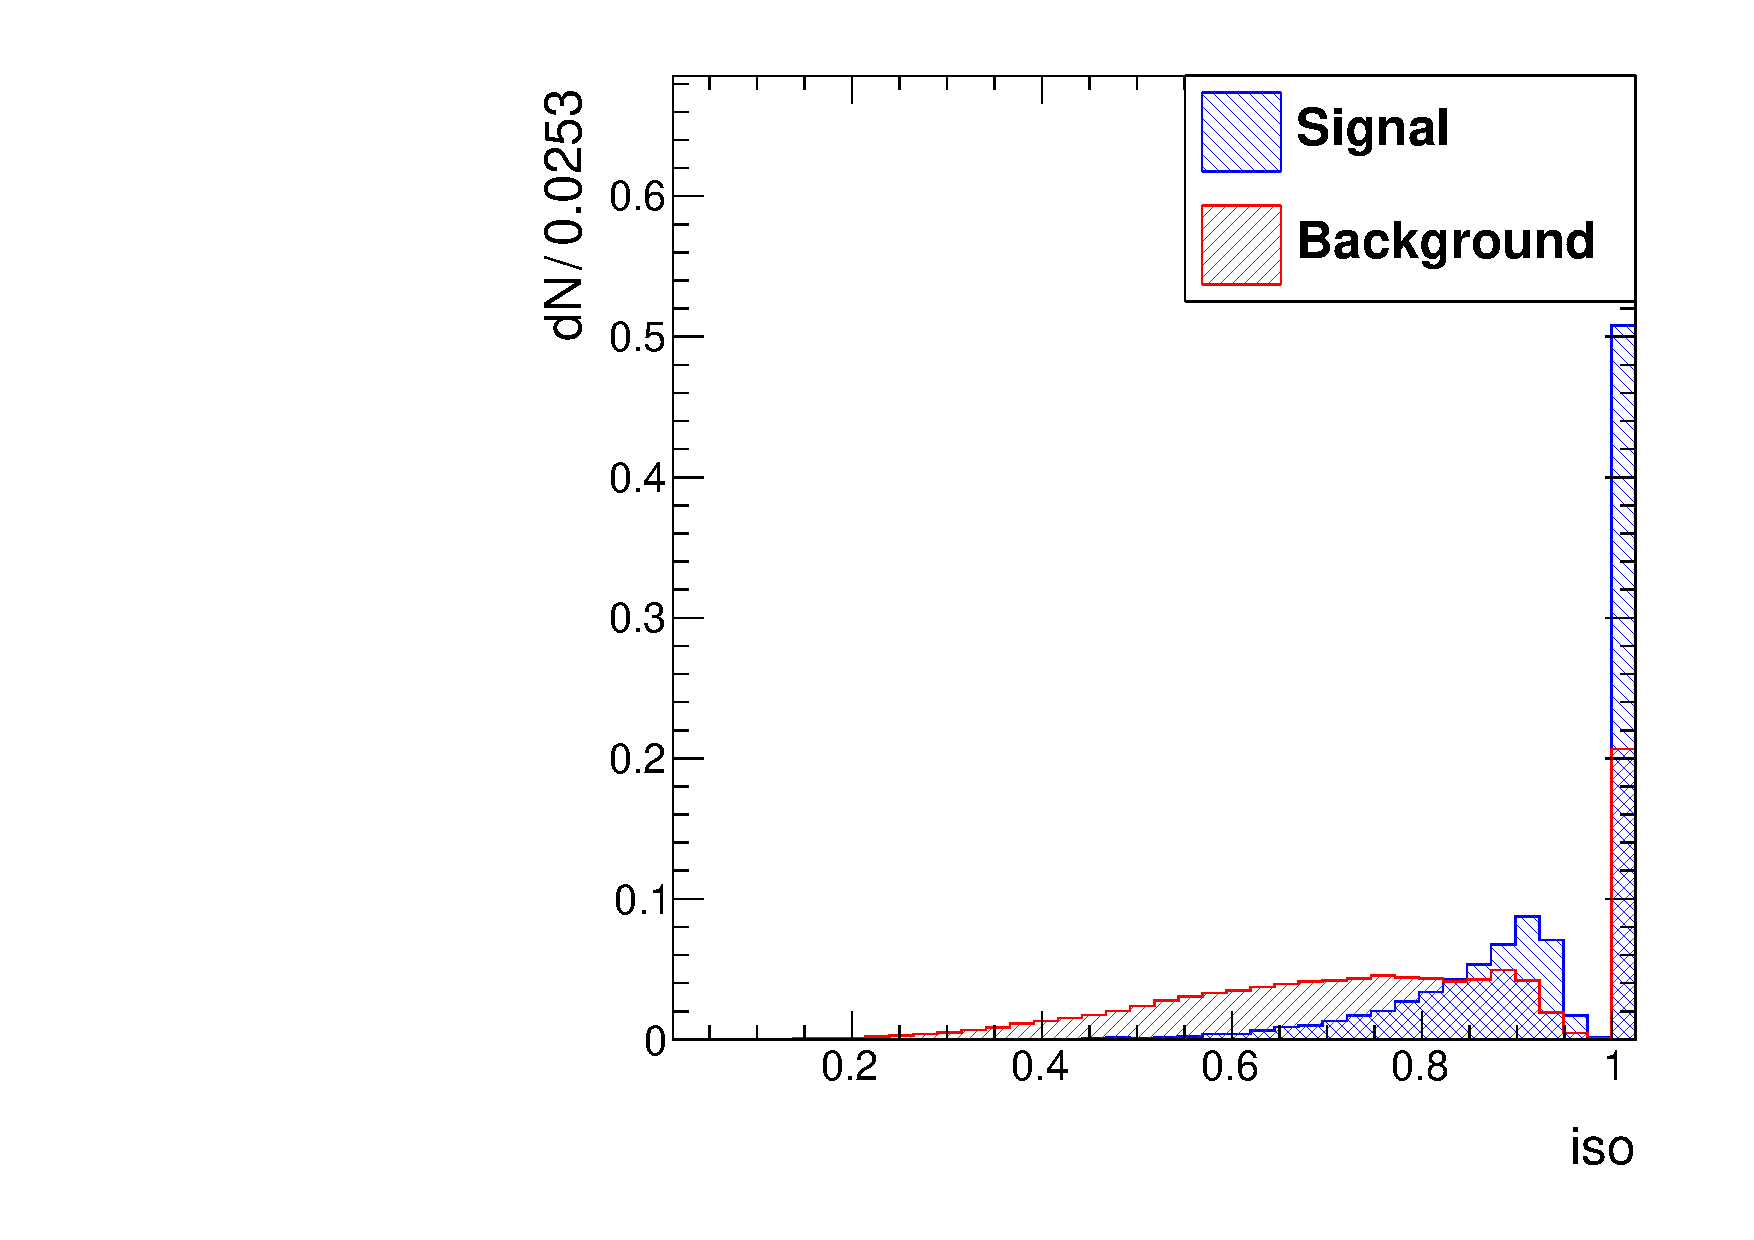
\includegraphics[width=\textwidth]{Figures/iso_endcaps}
                \label{fig:isoEndcaps}
        \end{subfigure}
        ~
        \begin{subfigure}[b]{0.2\textwidth}
                \centering
                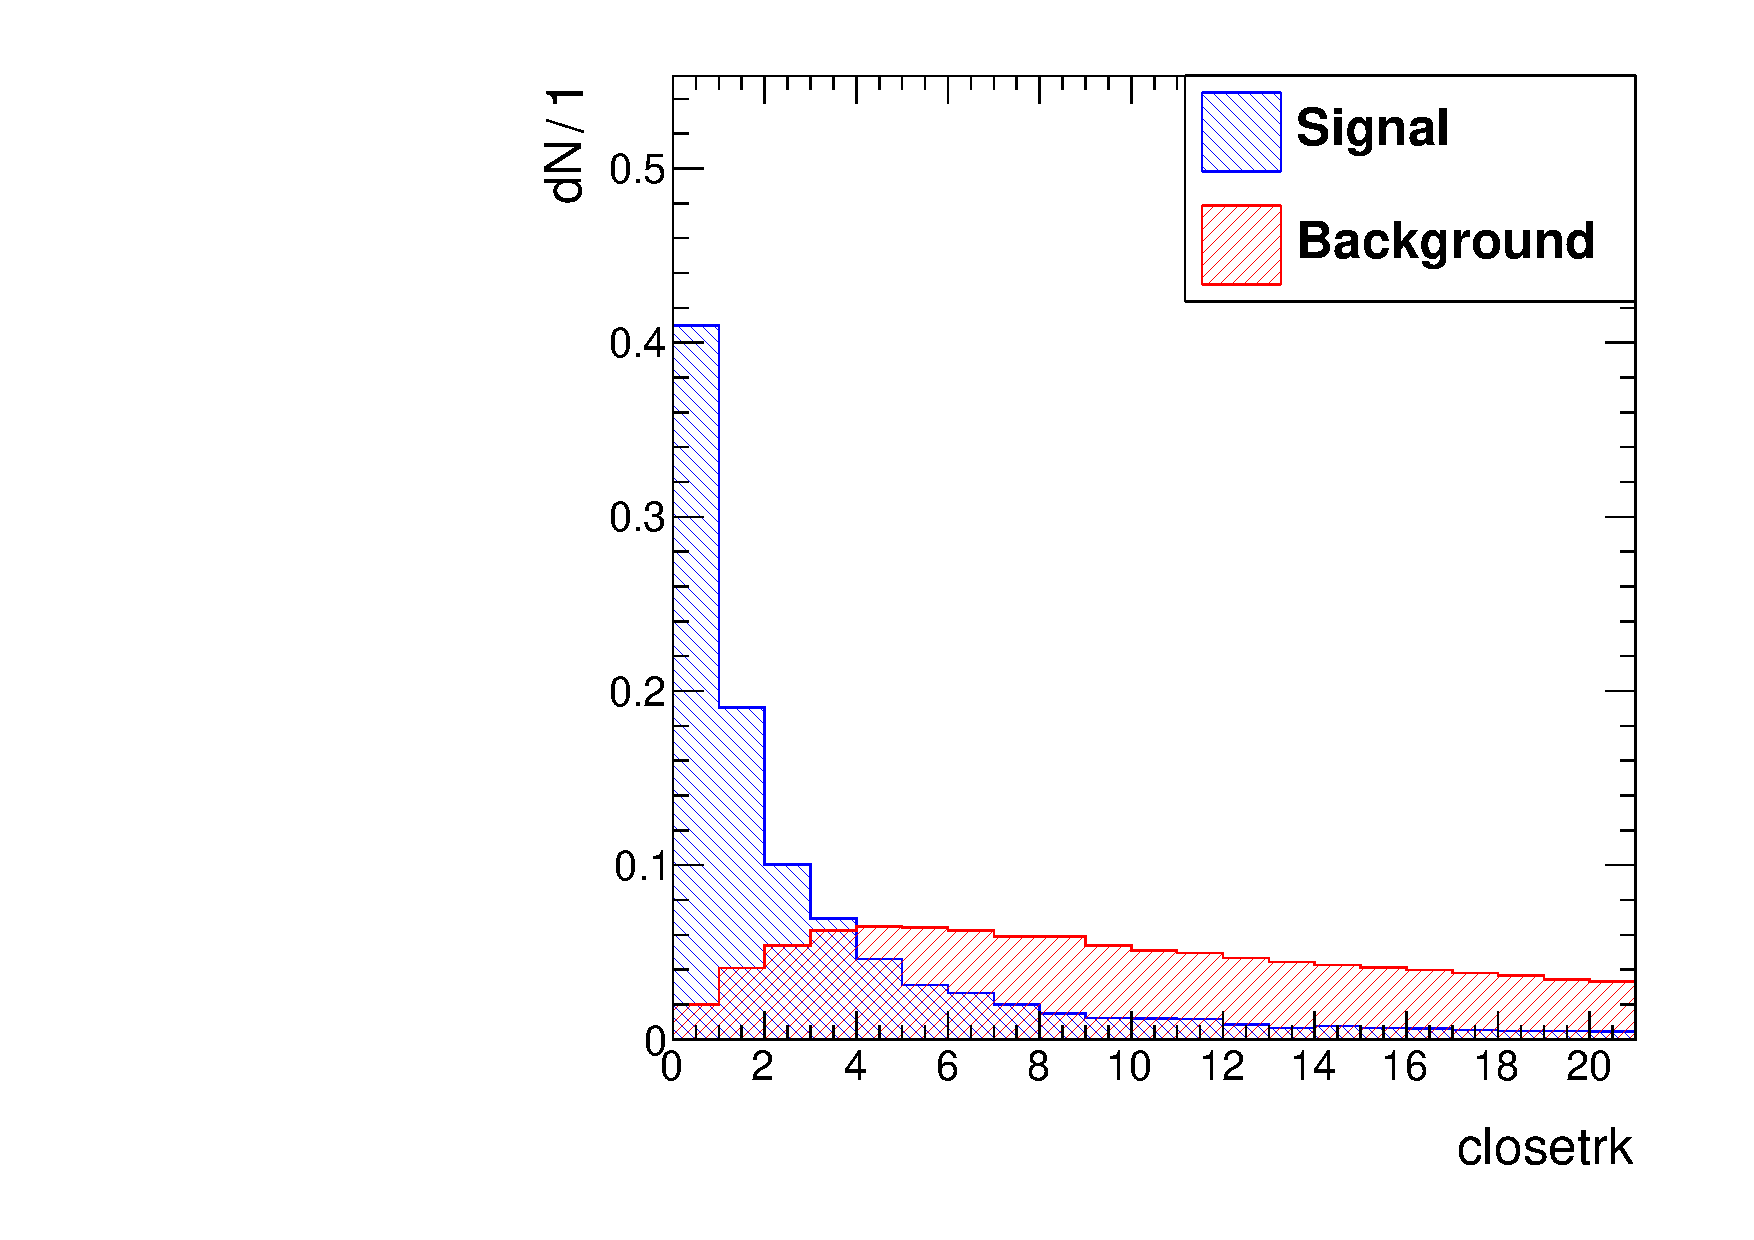
\includegraphics[width=\textwidth]{Figures/closetrk_endcaps}
                \label{fig:closetrkEndcaps}
        \end{subfigure}
        ~
        \begin{subfigure}[b]{0.2\textwidth}
                \centering
                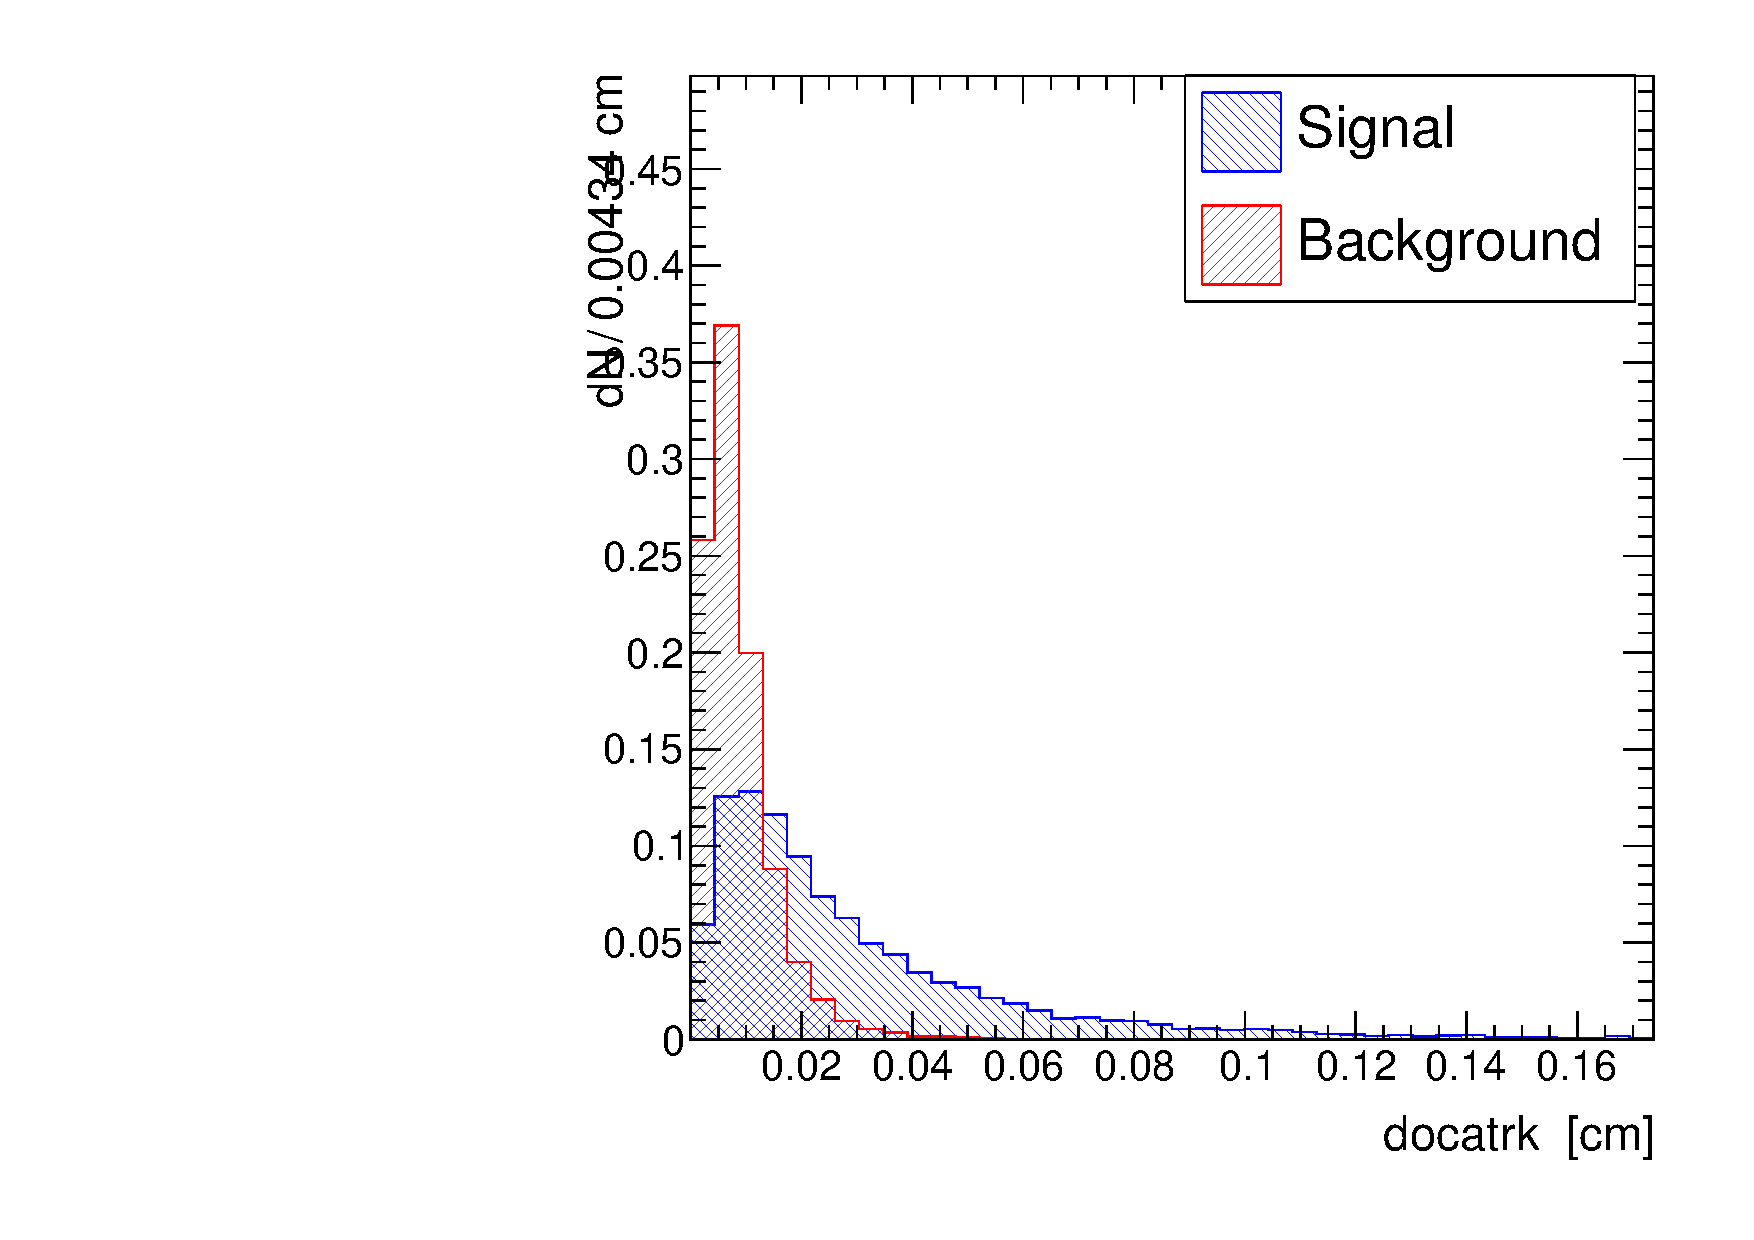
\includegraphics[width=\textwidth]{Figures/docatrk_endcaps}
                \label{fig:docatrkEndcaps}
        \end{subfigure}

        \begin{subfigure}[b]{0.2\textwidth}
                \centering
                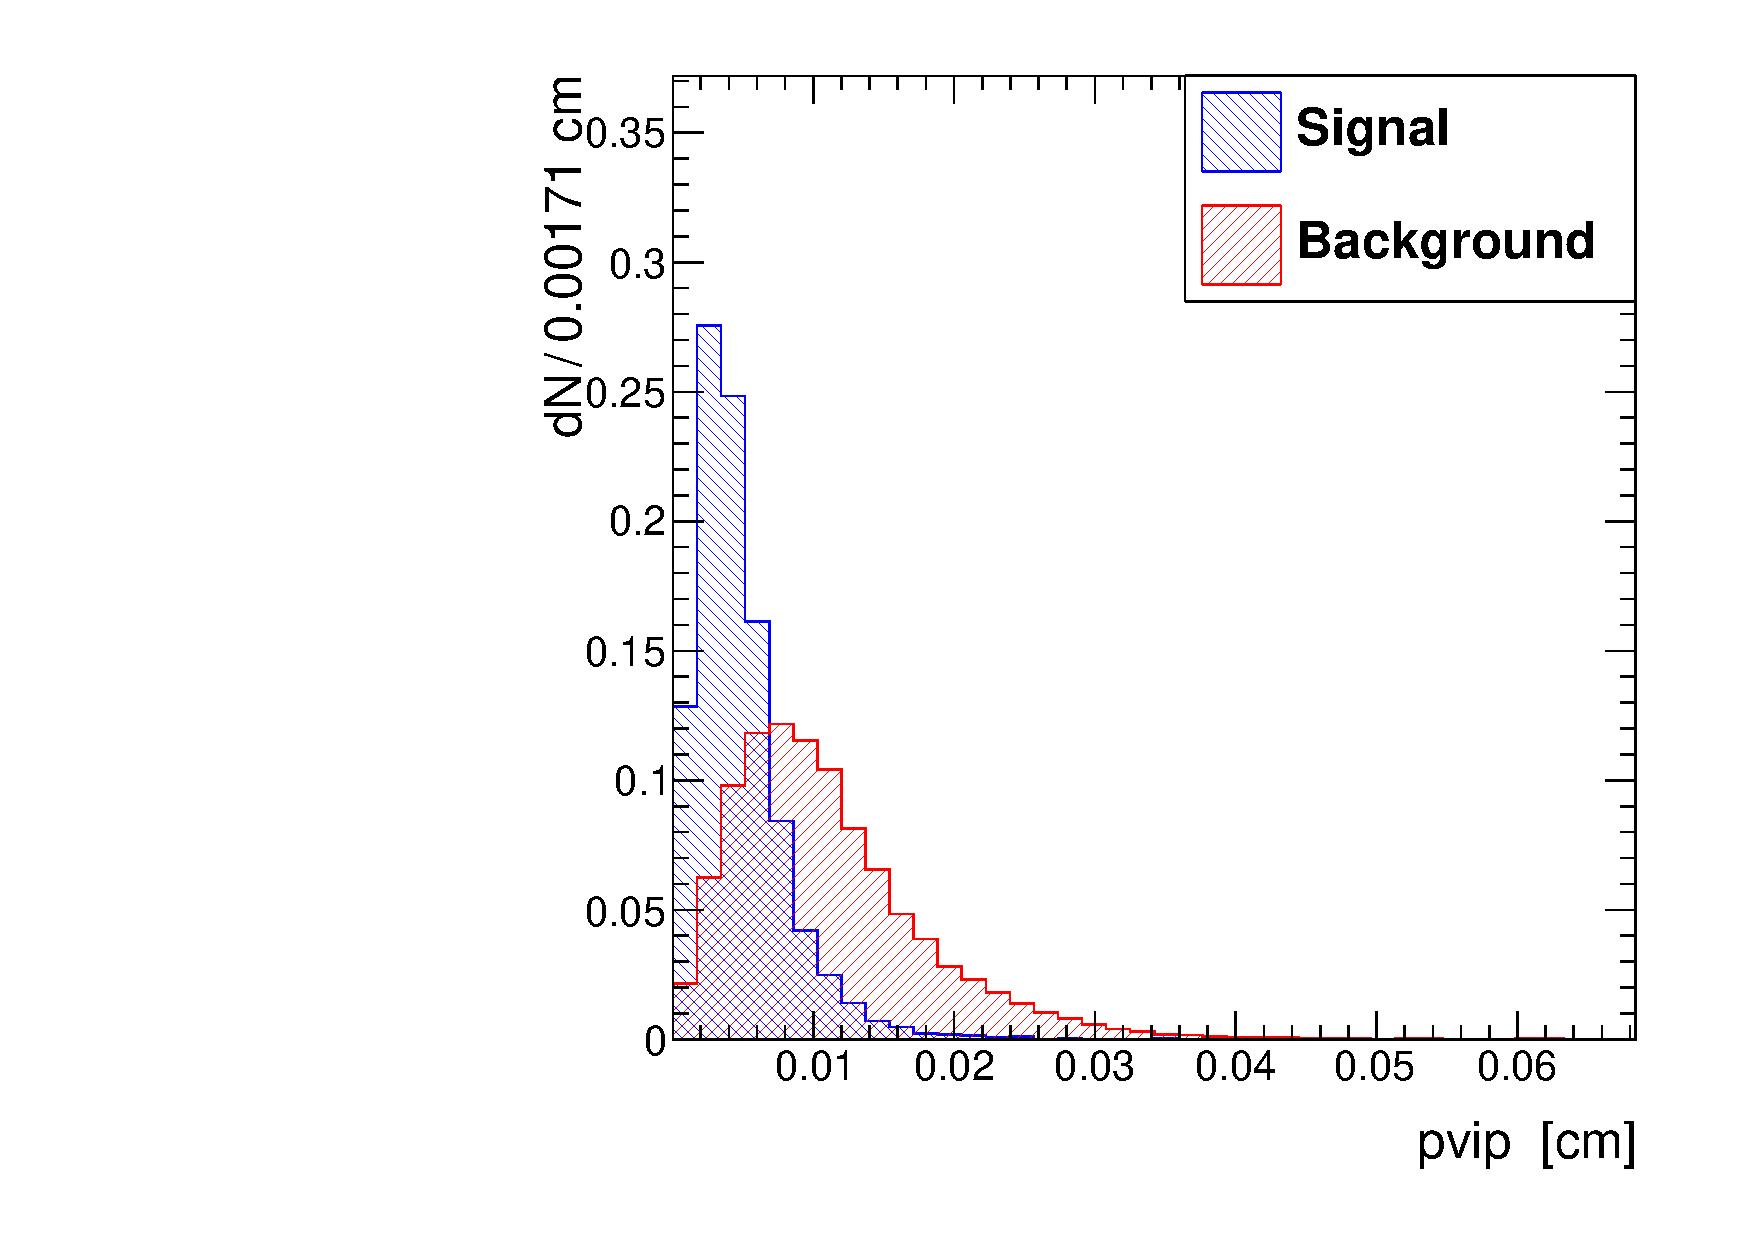
\includegraphics[width=\textwidth]{Figures/pvip_endcaps}
                \label{fig:pvipEndcaps}
        \end{subfigure}%
        ~
        \begin{subfigure}[b]{0.2\textwidth}
                \centering
                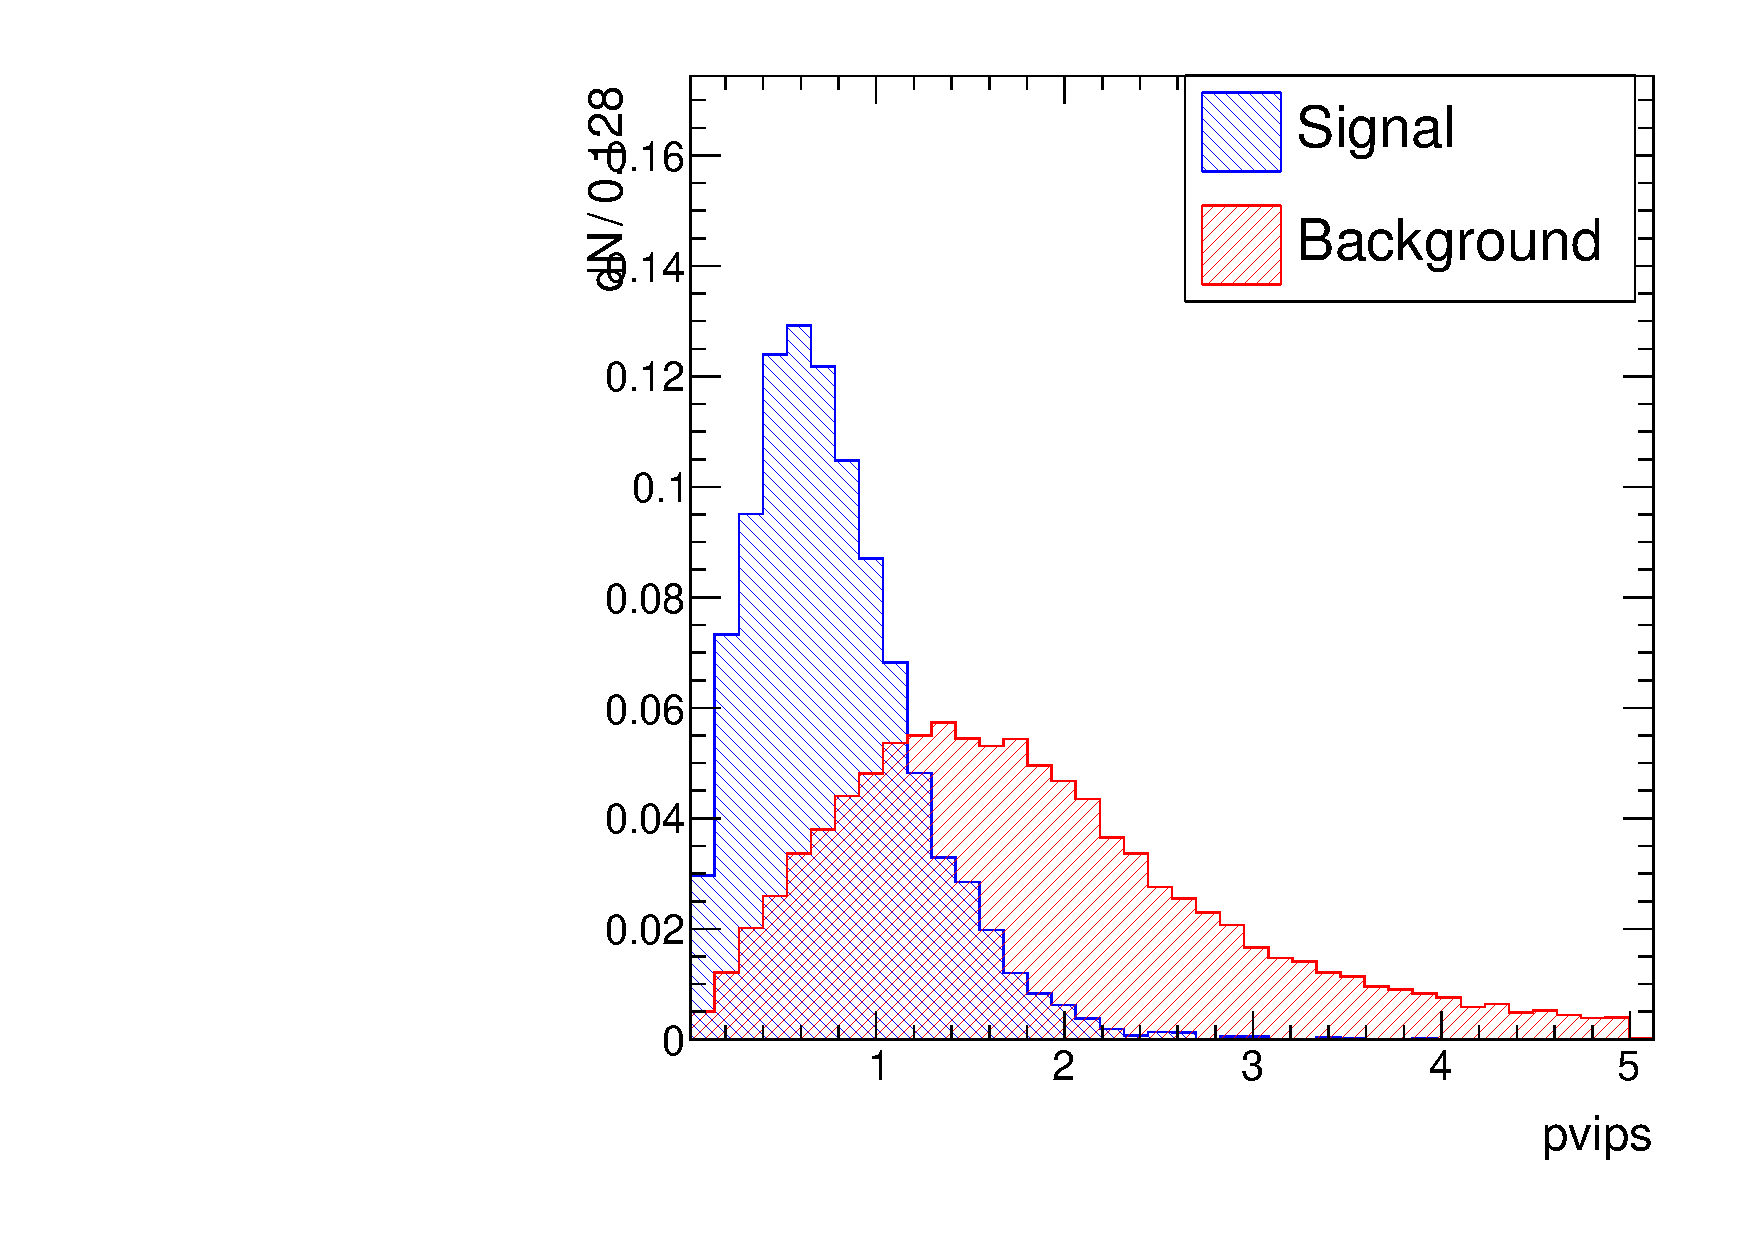
\includegraphics[width=\textwidth]{Figures/pvips_endcaps}
                \label{fig:pvipsEncaps}
        \end{subfigure}
        ~
        \begin{subfigure}[b]{0.2\textwidth}
                \centering
                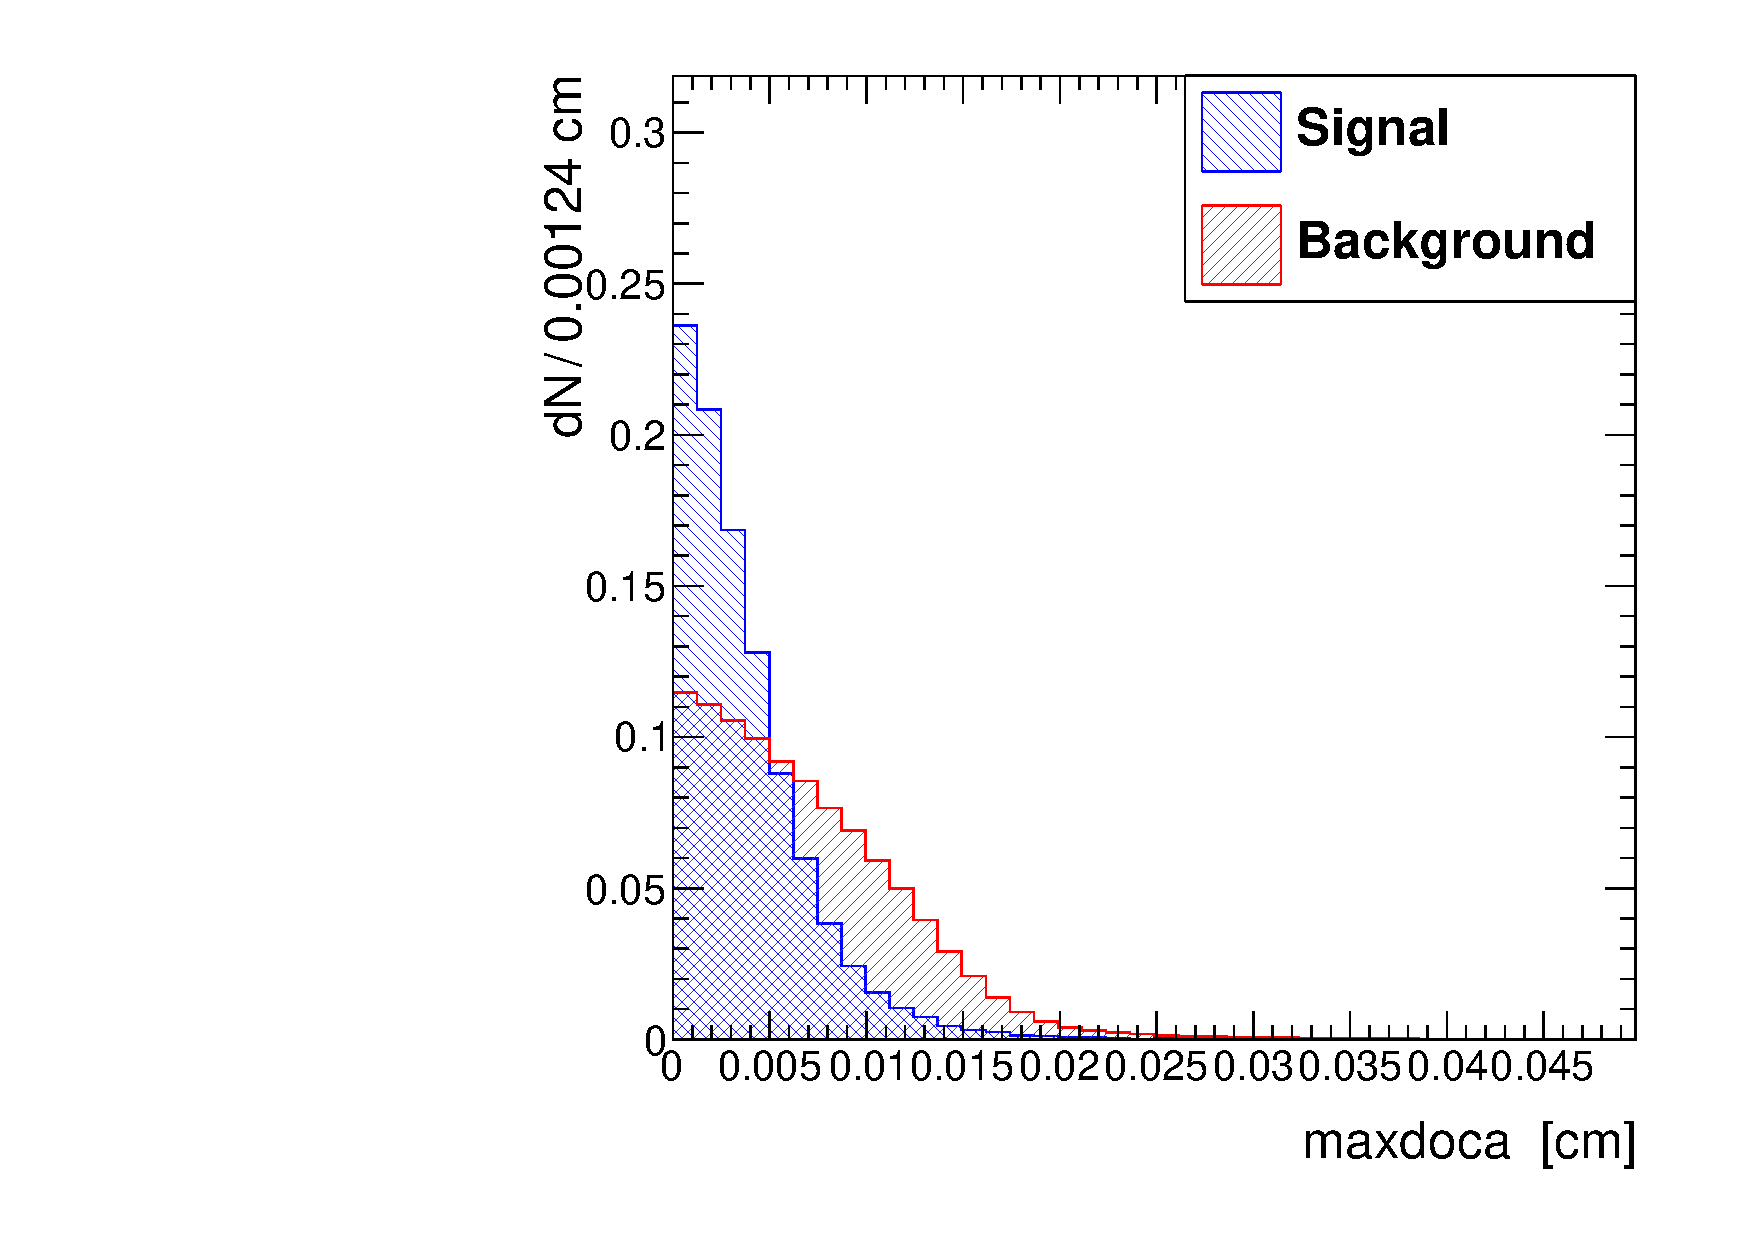
\includegraphics[width=\textwidth]{Figures/maxdoca_endcaps}
                \label{fig:maxdocaEndcaps}
        \end{subfigure}
        \caption{Standard TMVA plot of the input variables for the endcaps BDT for signal (blue) and background (red). The background is extracted from data dimuon sidebands.}
        \label{fig:TMVAPlotsEndcaps}
\end{sidewaysfigure}


\subsection{variable ranking and correlations}

\begin{figure}
		\centering
        \begin{subfigure}[b]{0.45\textwidth}
				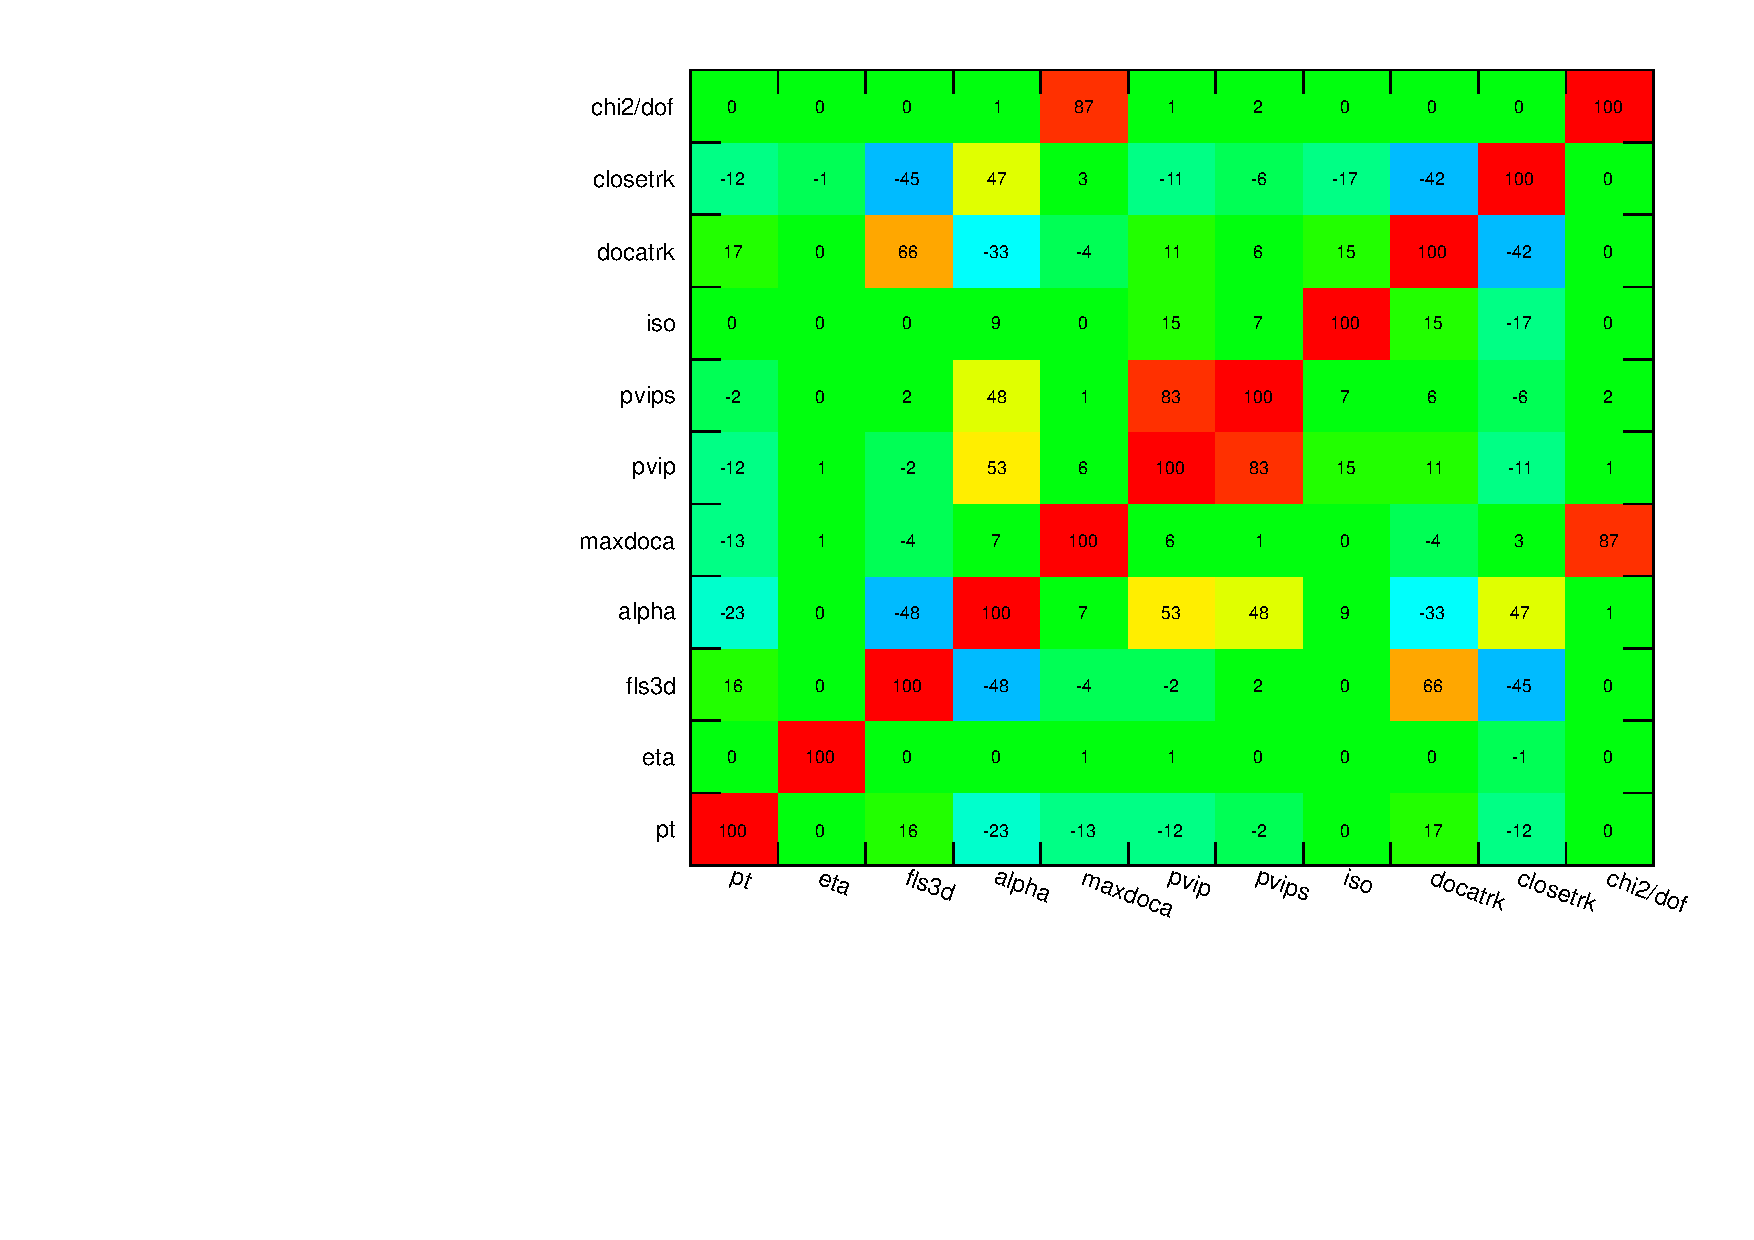
\includegraphics[width=\textwidth]{Figures/correlationMatrixS_barrel}
				\label{fig:matrixSBarrel}
        \end{subfigure}
        ~
        \begin{subfigure}[b]{0.45\textwidth}
				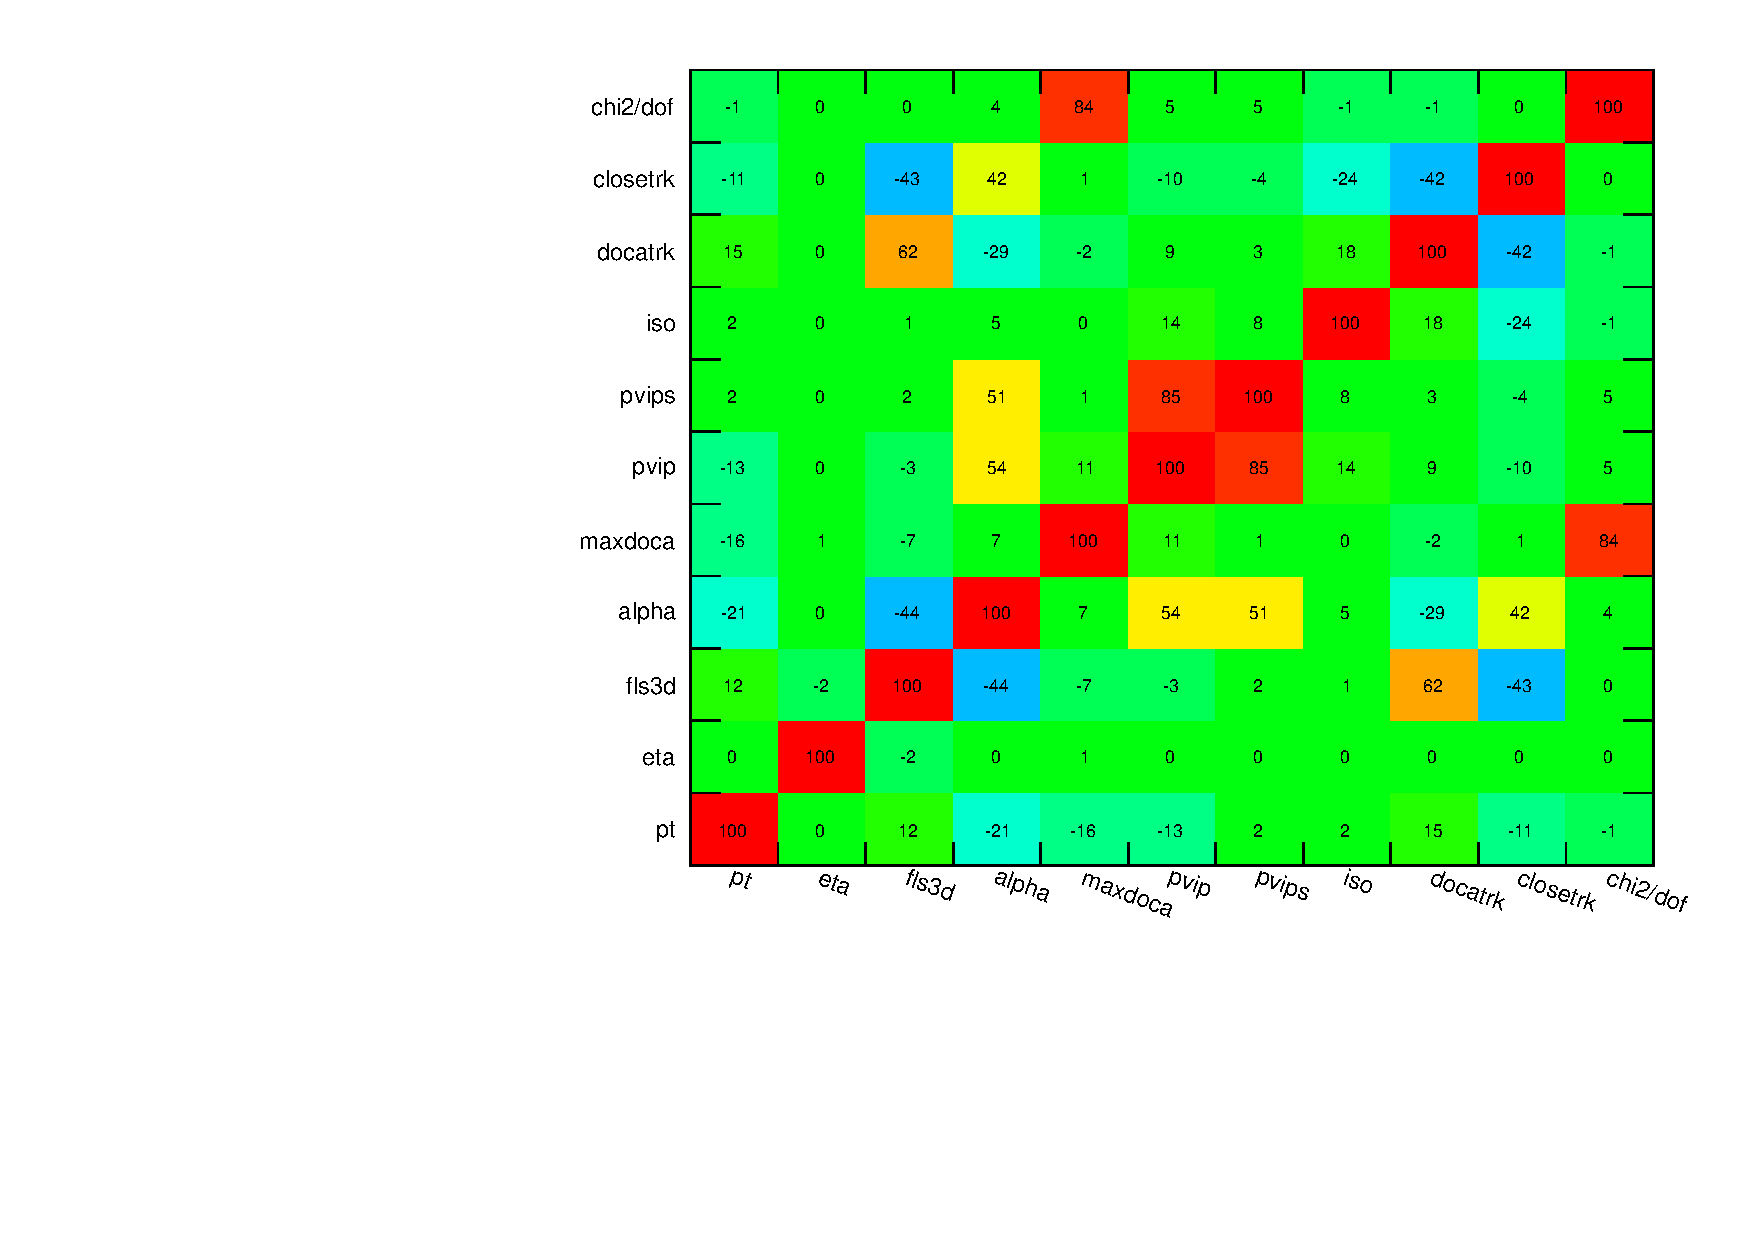
\includegraphics[width=\textwidth]{Figures/correlationMatrixS_endcaps}
				\label{fig:matrixSEndcaps}
        \end{subfigure}
        \caption{Correlation matrix for signal events in the barrel (left) and the endcap (right).}
        \label{fig:correlationMatricesSignal}
\end{figure}

\begin{figure}
		\centering
        \begin{subfigure}[b]{0.45\textwidth}
				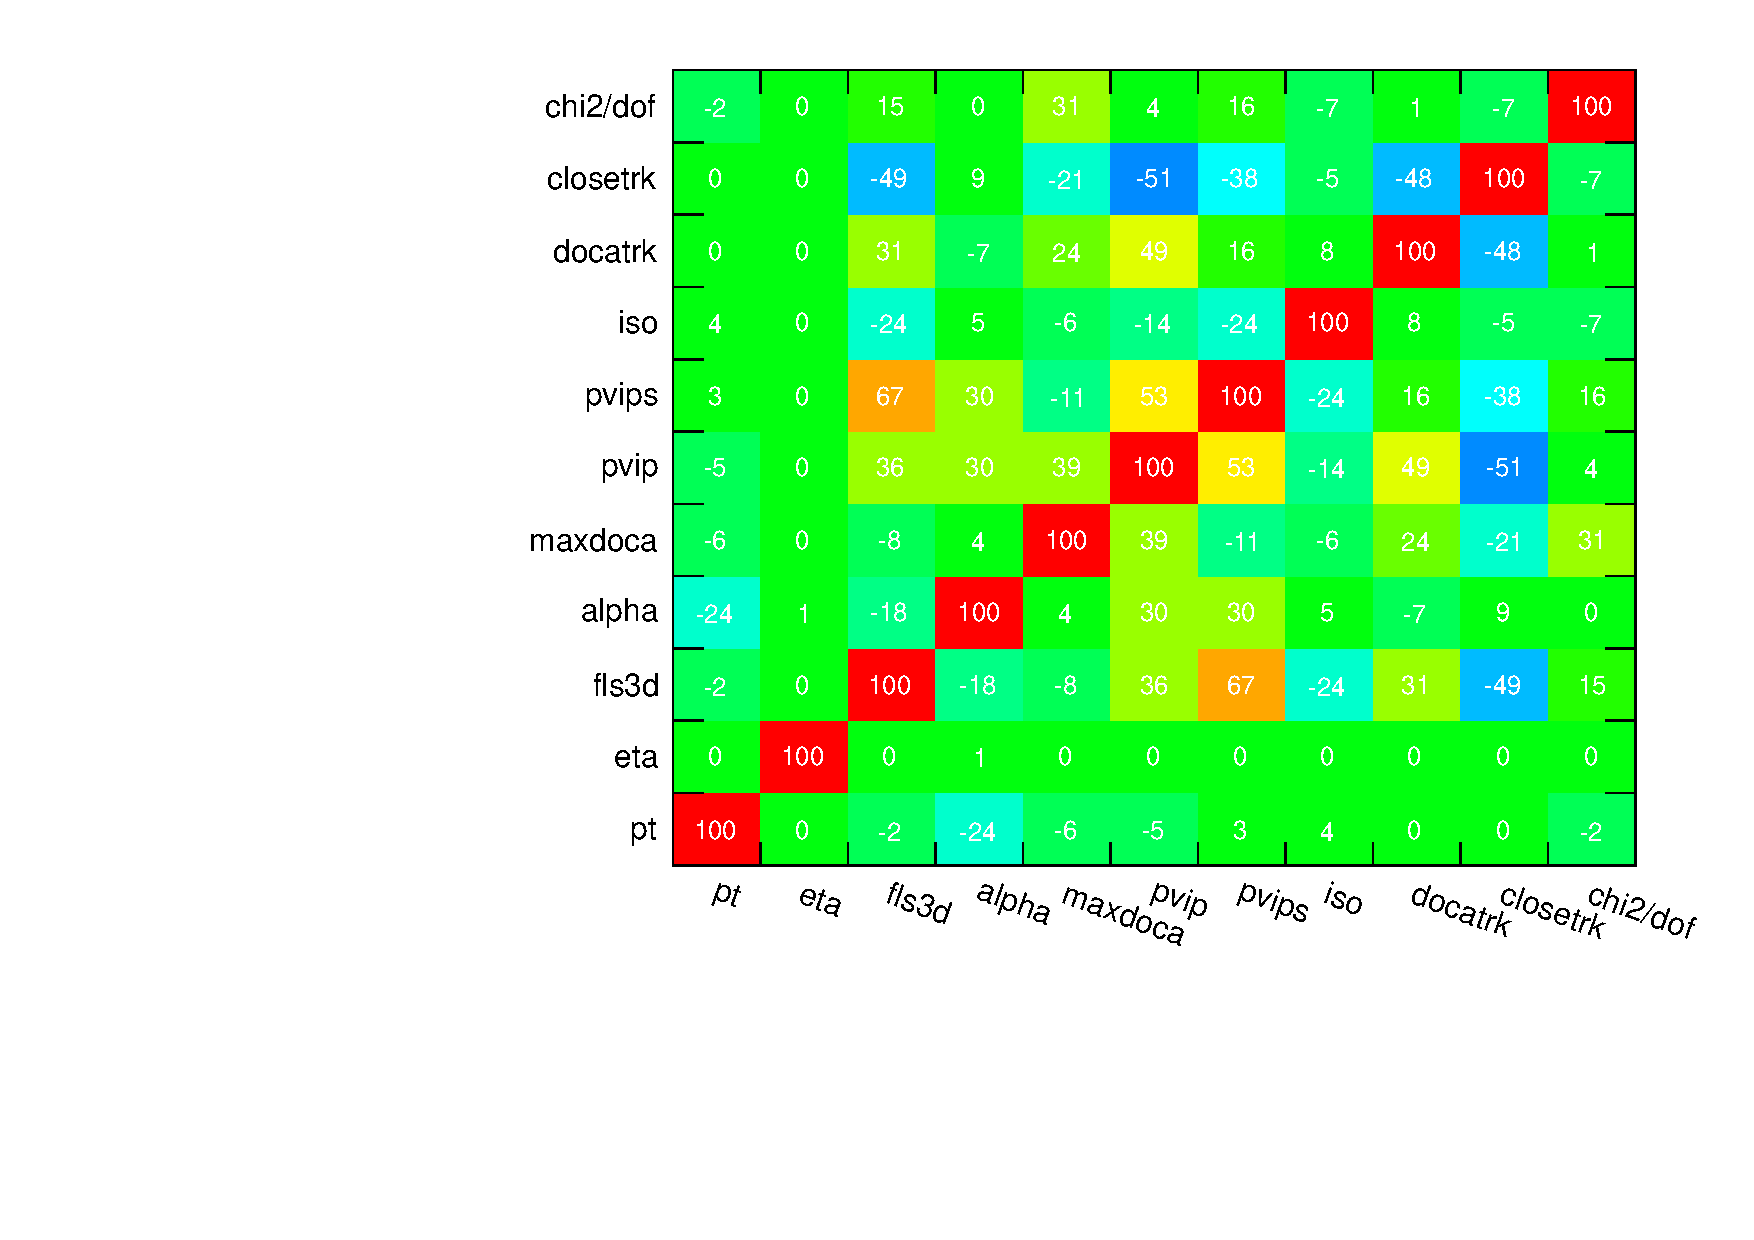
\includegraphics[width=\textwidth]{Figures/correlationMatrixB_barrel}
				\label{fig:matrixBBarrel}
        \end{subfigure}
        ~
        \begin{subfigure}[b]{0.45\textwidth}
				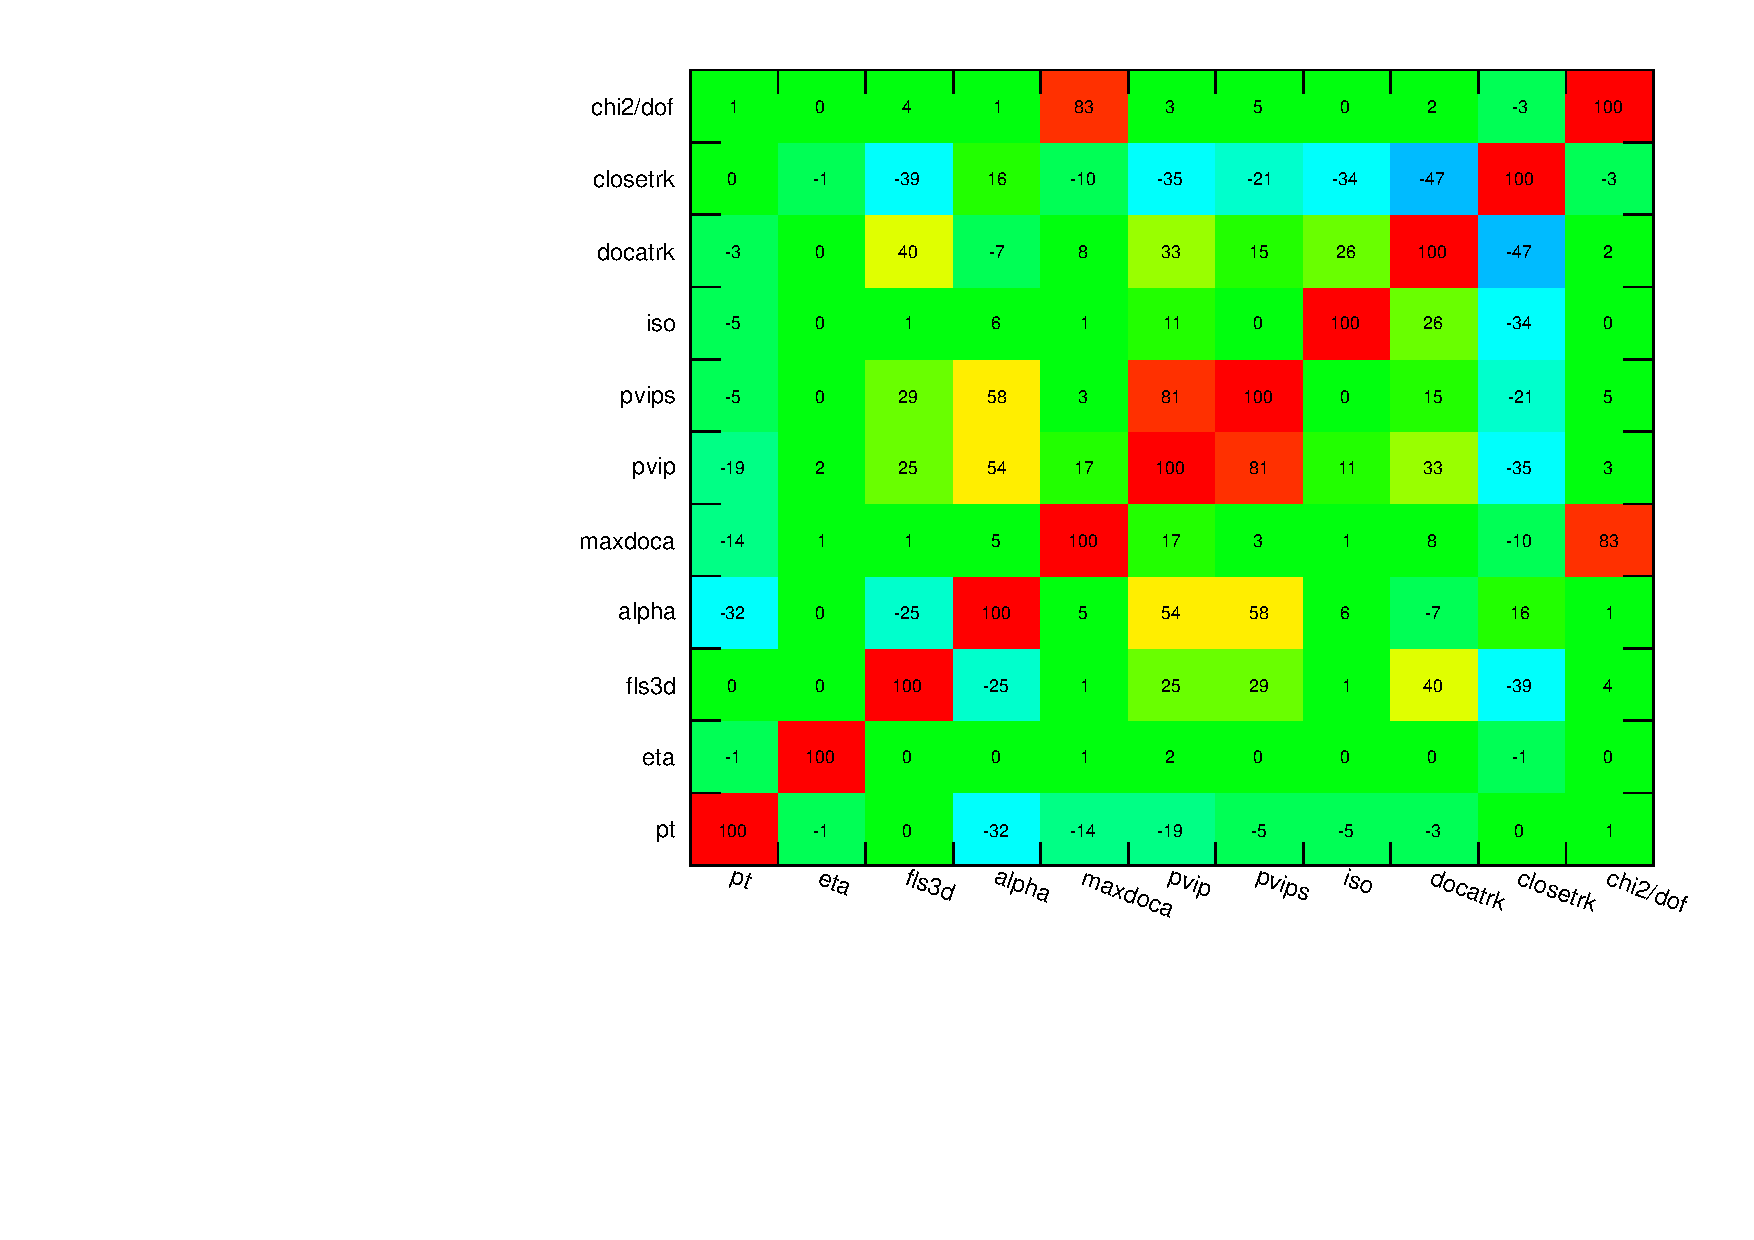
\includegraphics[width=\textwidth]{Figures/correlationMatrixB_endcaps}
				\label{fig:matrixBEndcaps}
        \end{subfigure}
        \caption{Correlation matrix for background events in the barrel (left) and the endcap (right).}
        \label{fig:correlationMatricesBackground}
\end{figure}

Tables \ref{tab:datasetsbarrelIdTransformation} and \ref{tab:datasetsendcapsIdTransformation} show the ranking of variables before
the BDT training.
\input{Tables/ranking_barrel_IdTransformation.txt}
\input{Tables/ranking_endcaps_IdTransformation.txt}

\begin{figure}
  \centering
  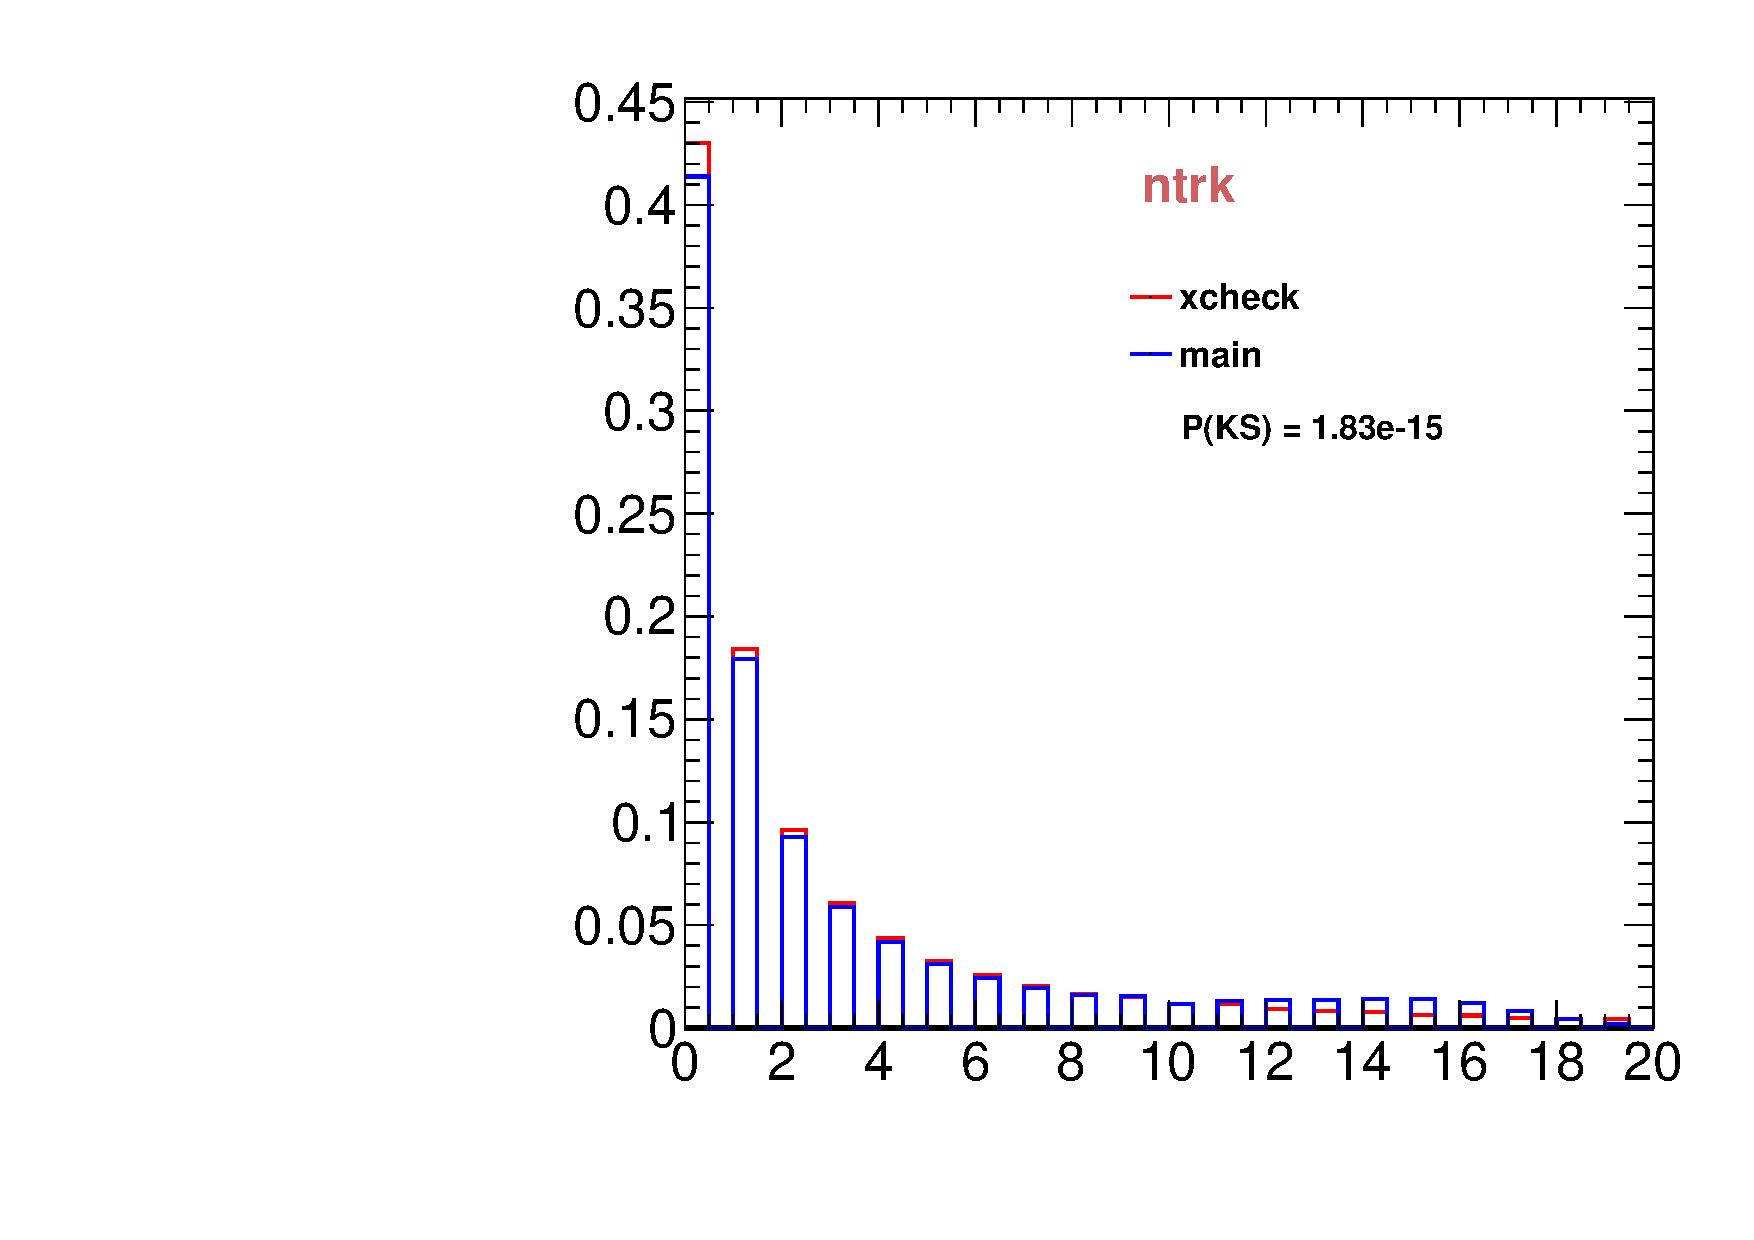
\includegraphics[width=0.3\textwidth]{Figures/VariablesComparison/MC_barrel_figs/closetrk}
  %\label{fig:MC_barrel_closetrk}
  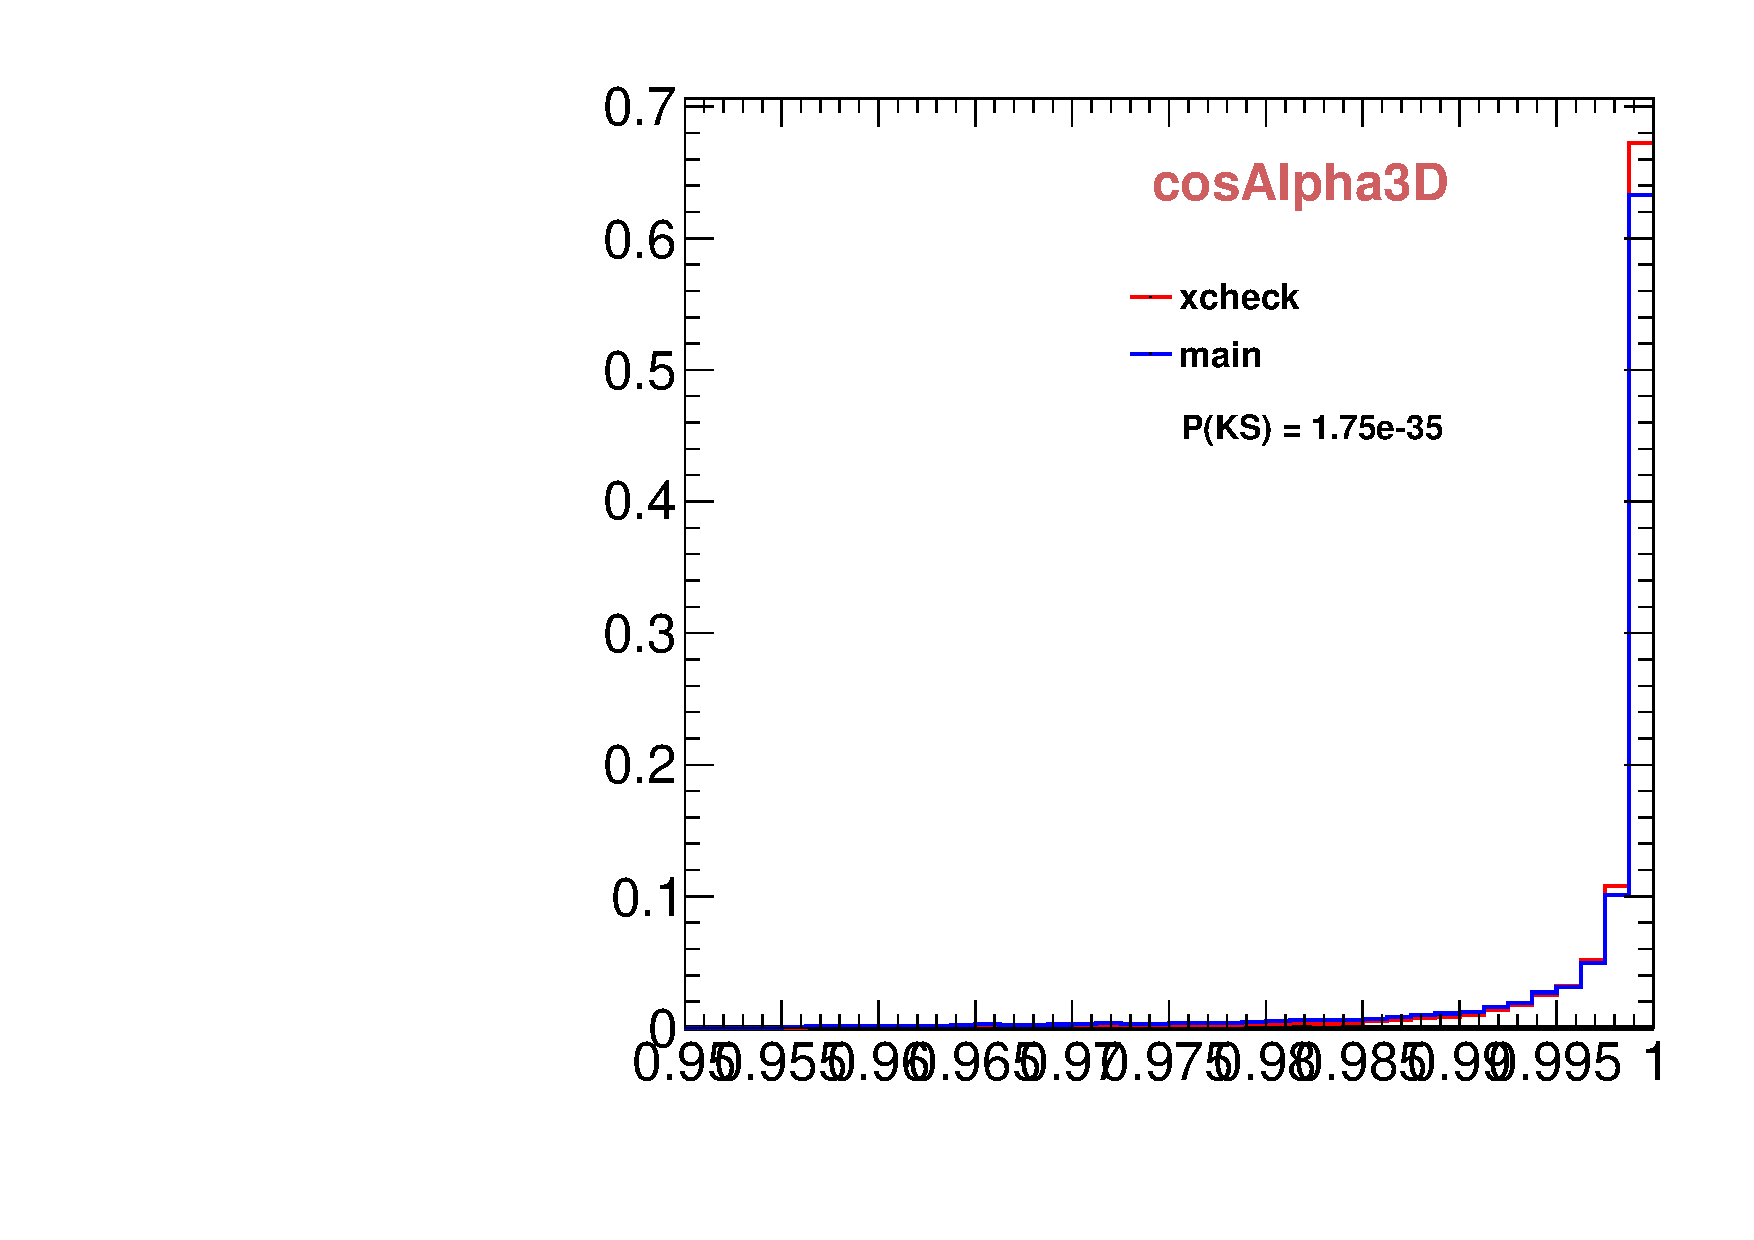
\includegraphics[width=0.3\textwidth]{Figures/VariablesComparison/MC_barrel_figs/cosa}
  %\label{fig:MC_barrel_cosa}
  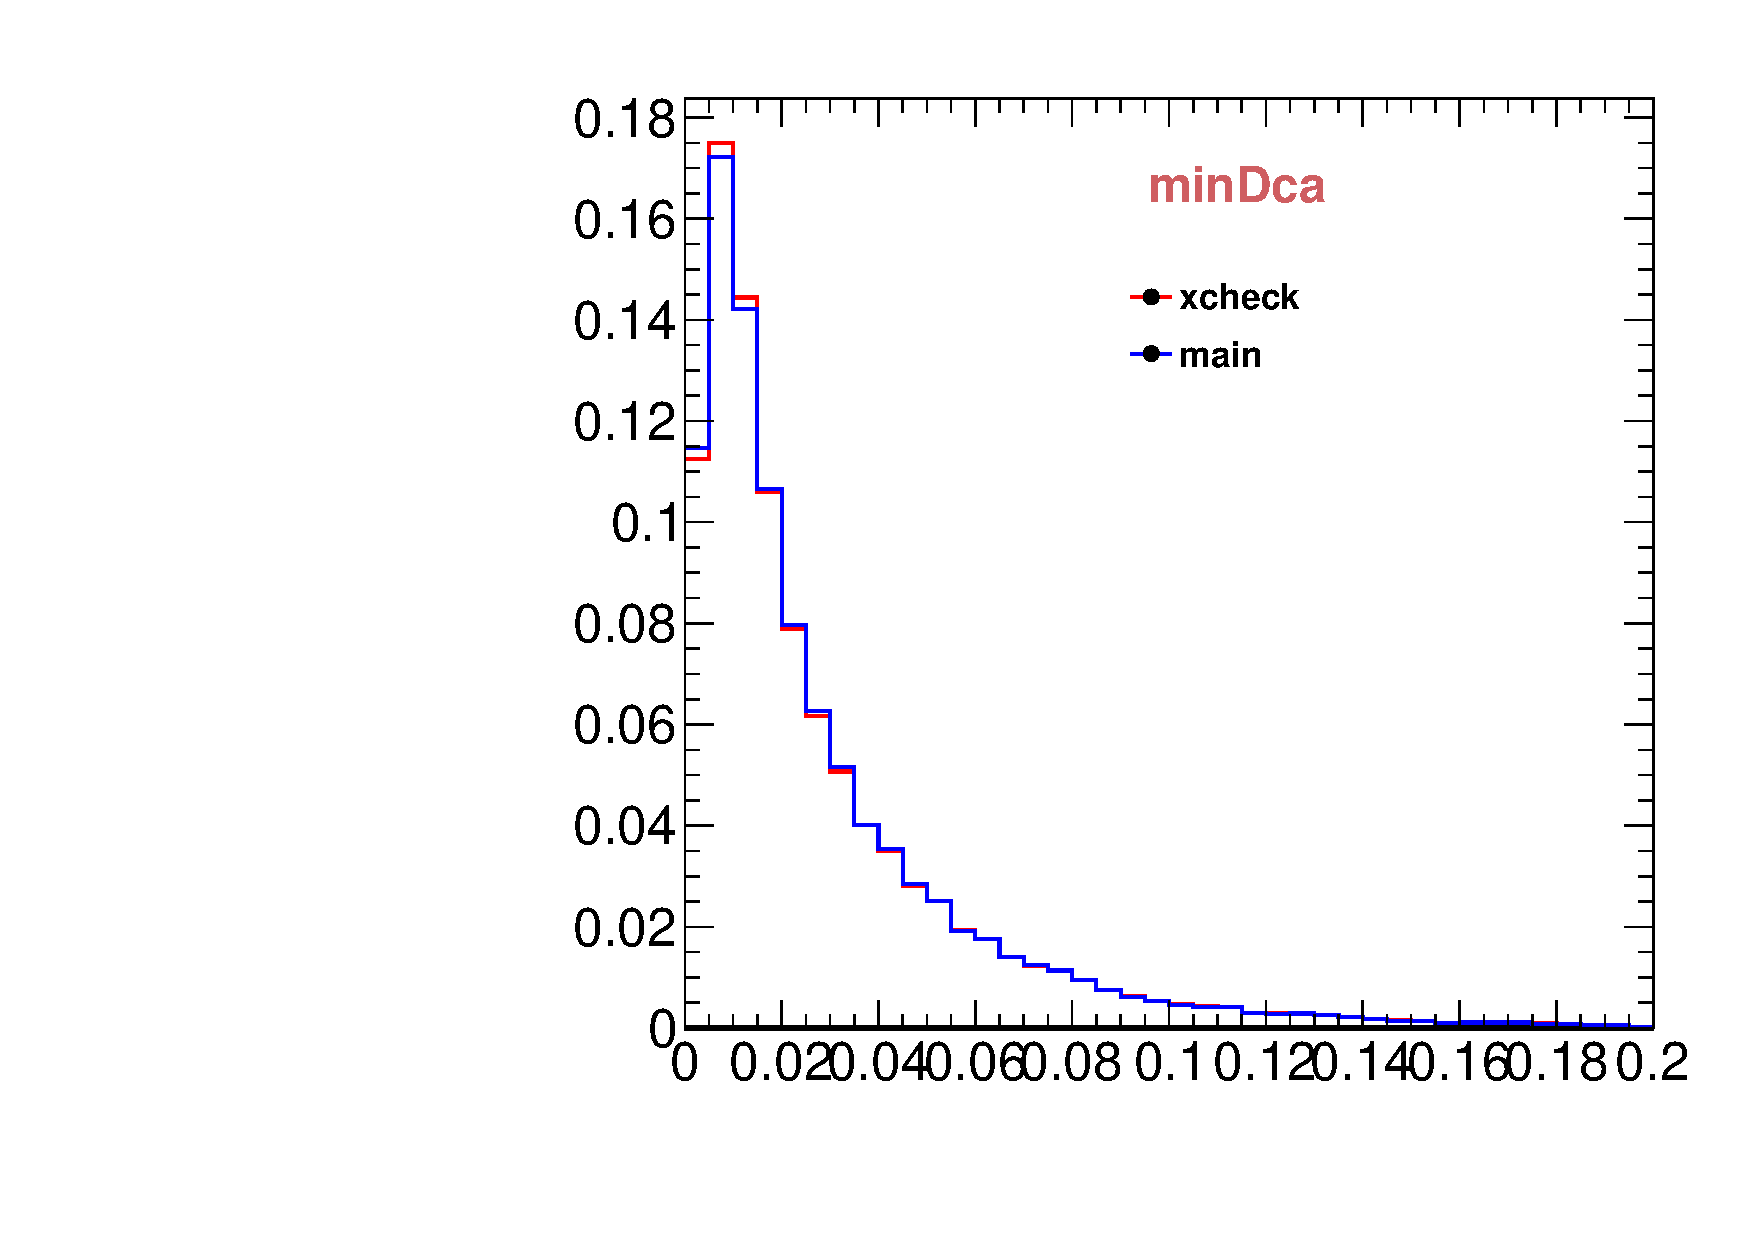
\includegraphics[width=0.3\textwidth]{Figures/VariablesComparison/MC_barrel_figs/docatrk}
  %\label{fig:MC_barrel_docatrk}
  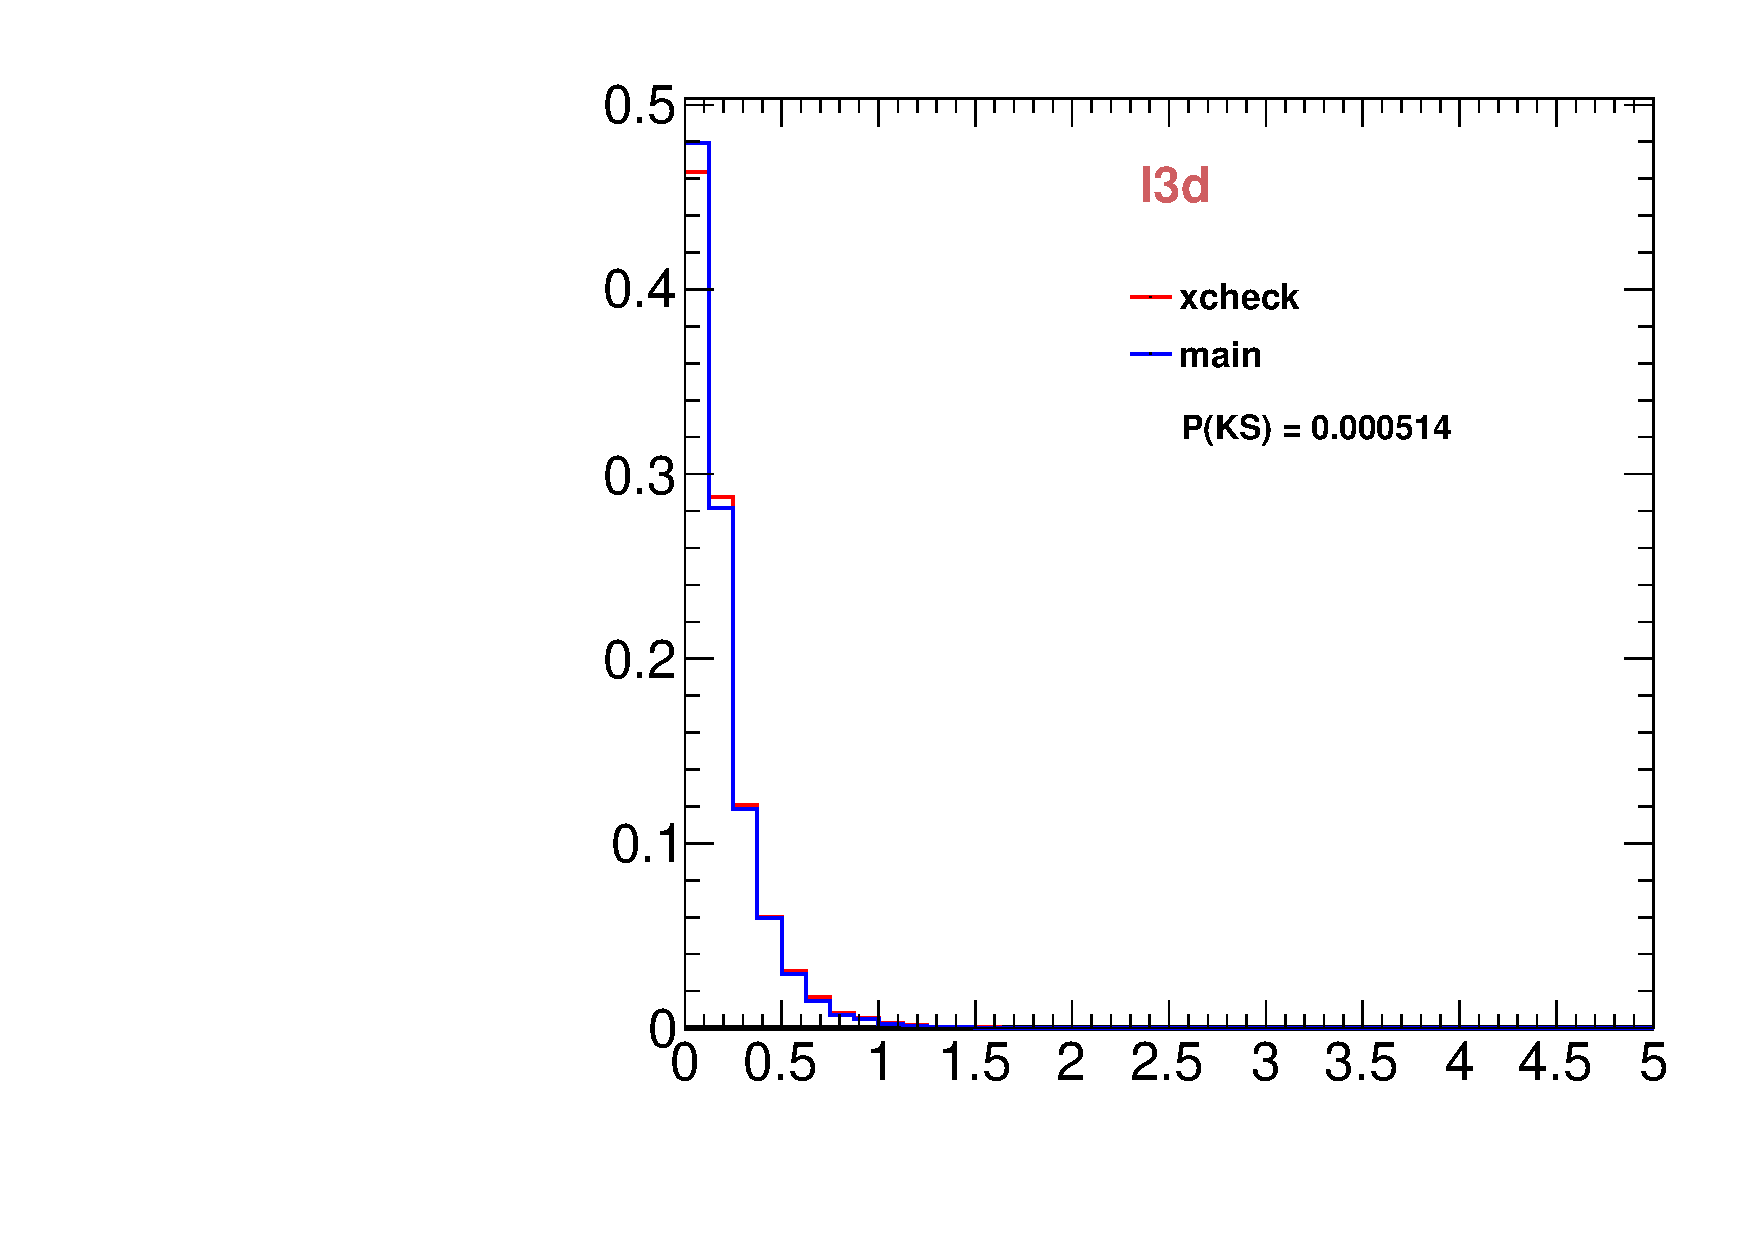
\includegraphics[width=0.3\textwidth]{Figures/VariablesComparison/MC_barrel_figs/fl3d}
  %\label{fig:MC_barrel_fl3d}
  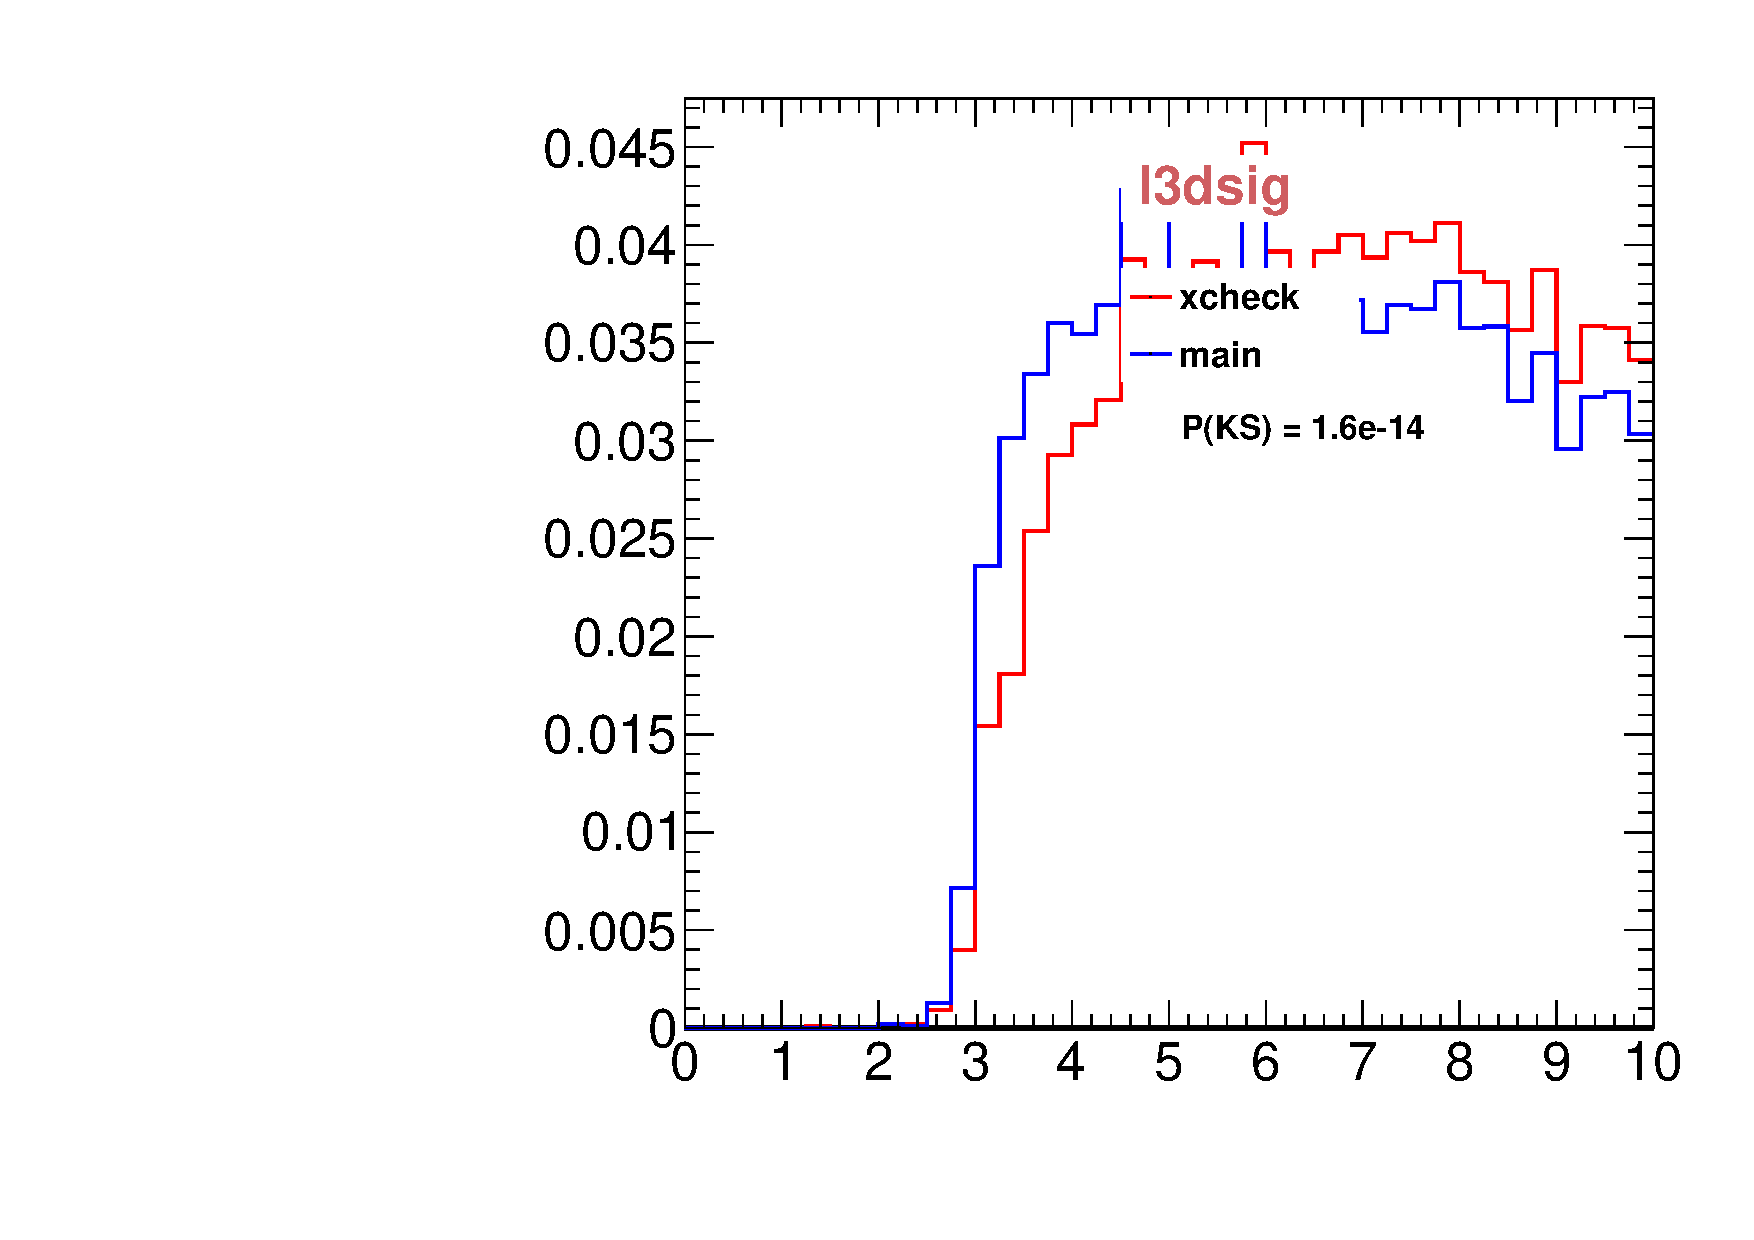
\includegraphics[width=0.3\textwidth]{Figures/VariablesComparison/MC_barrel_figs/fls3d}
  %\label{fig:MC_barrel_fls3d}
  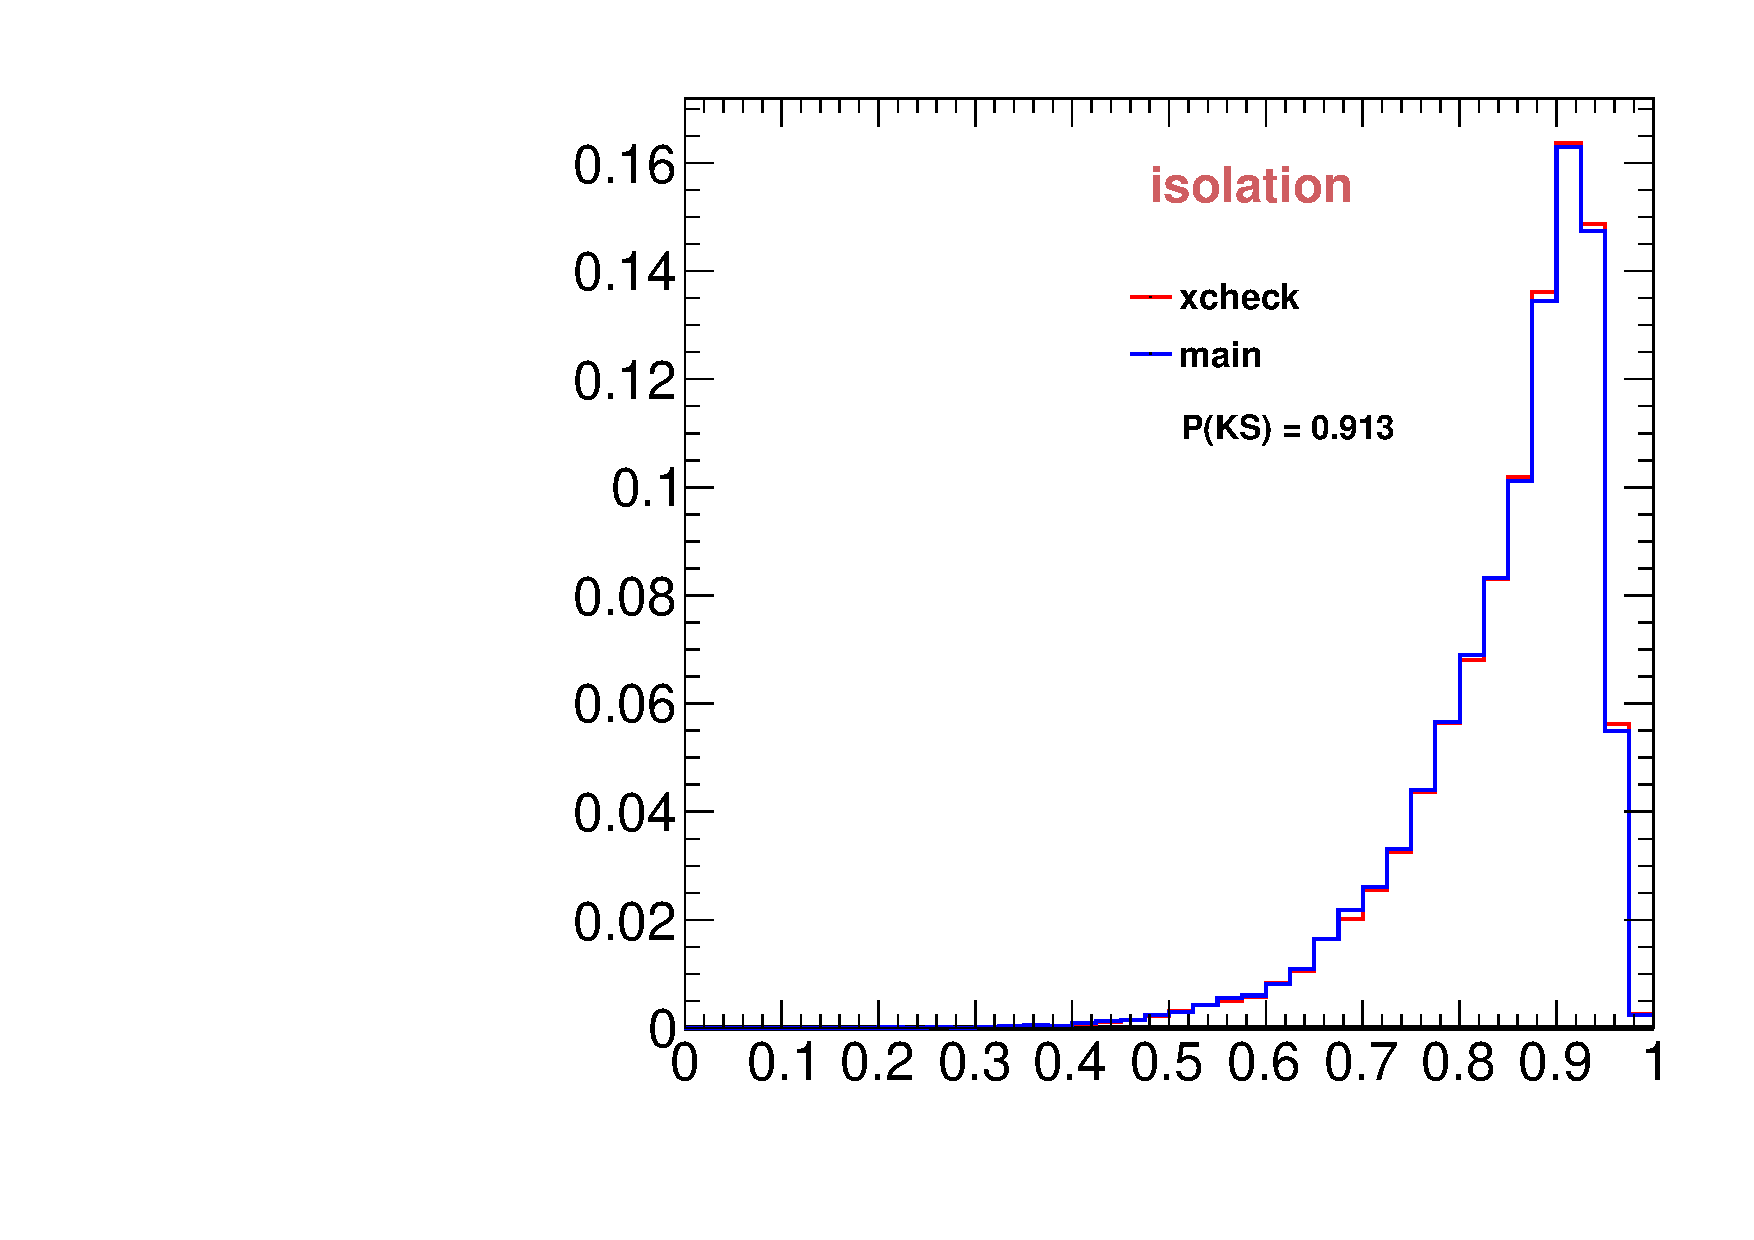
\includegraphics[width=0.3\textwidth]{Figures/VariablesComparison/MC_barrel_figs/iso}
  %\label{fig:MC_barrel_iso}
  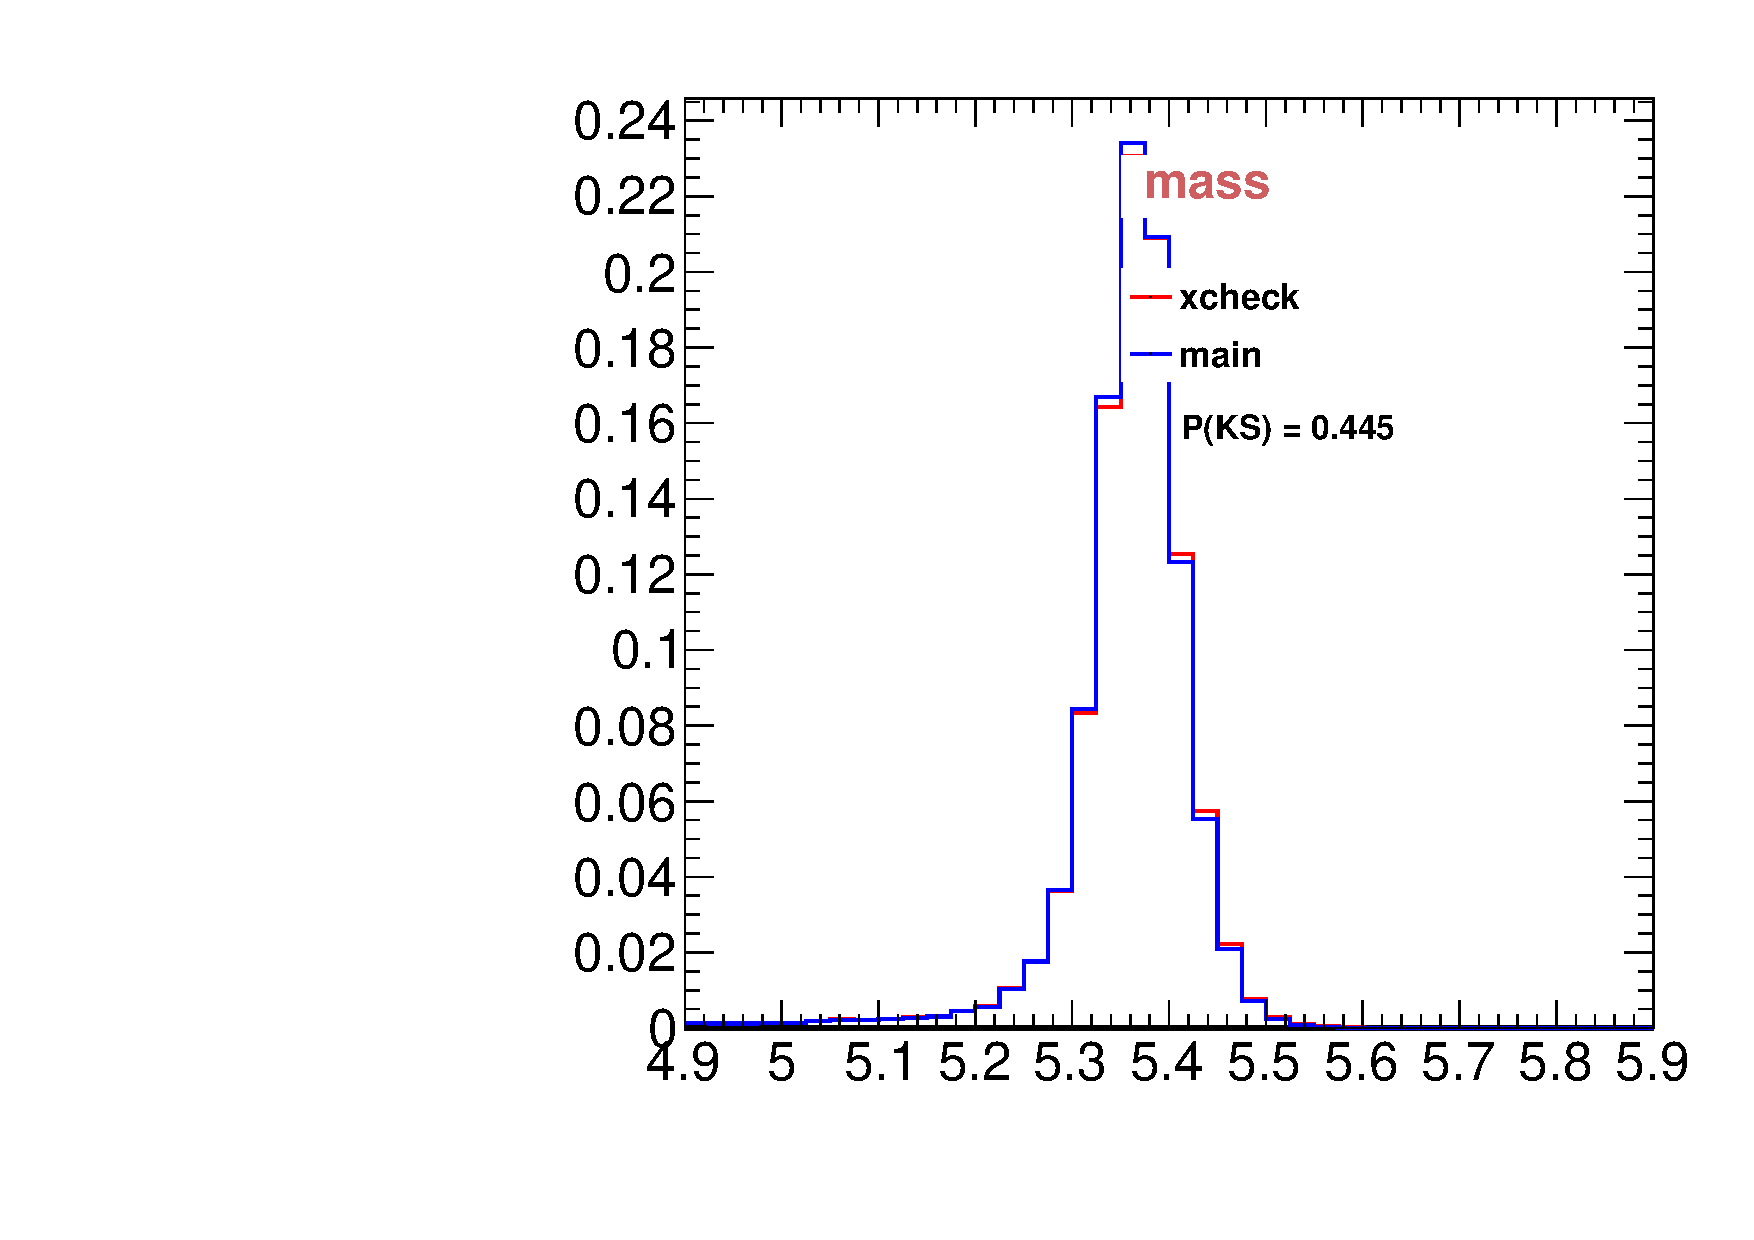
\includegraphics[width=0.3\textwidth]{Figures/VariablesComparison/MC_barrel_figs/m}
  %\label{fig:MC_barrel_m}
  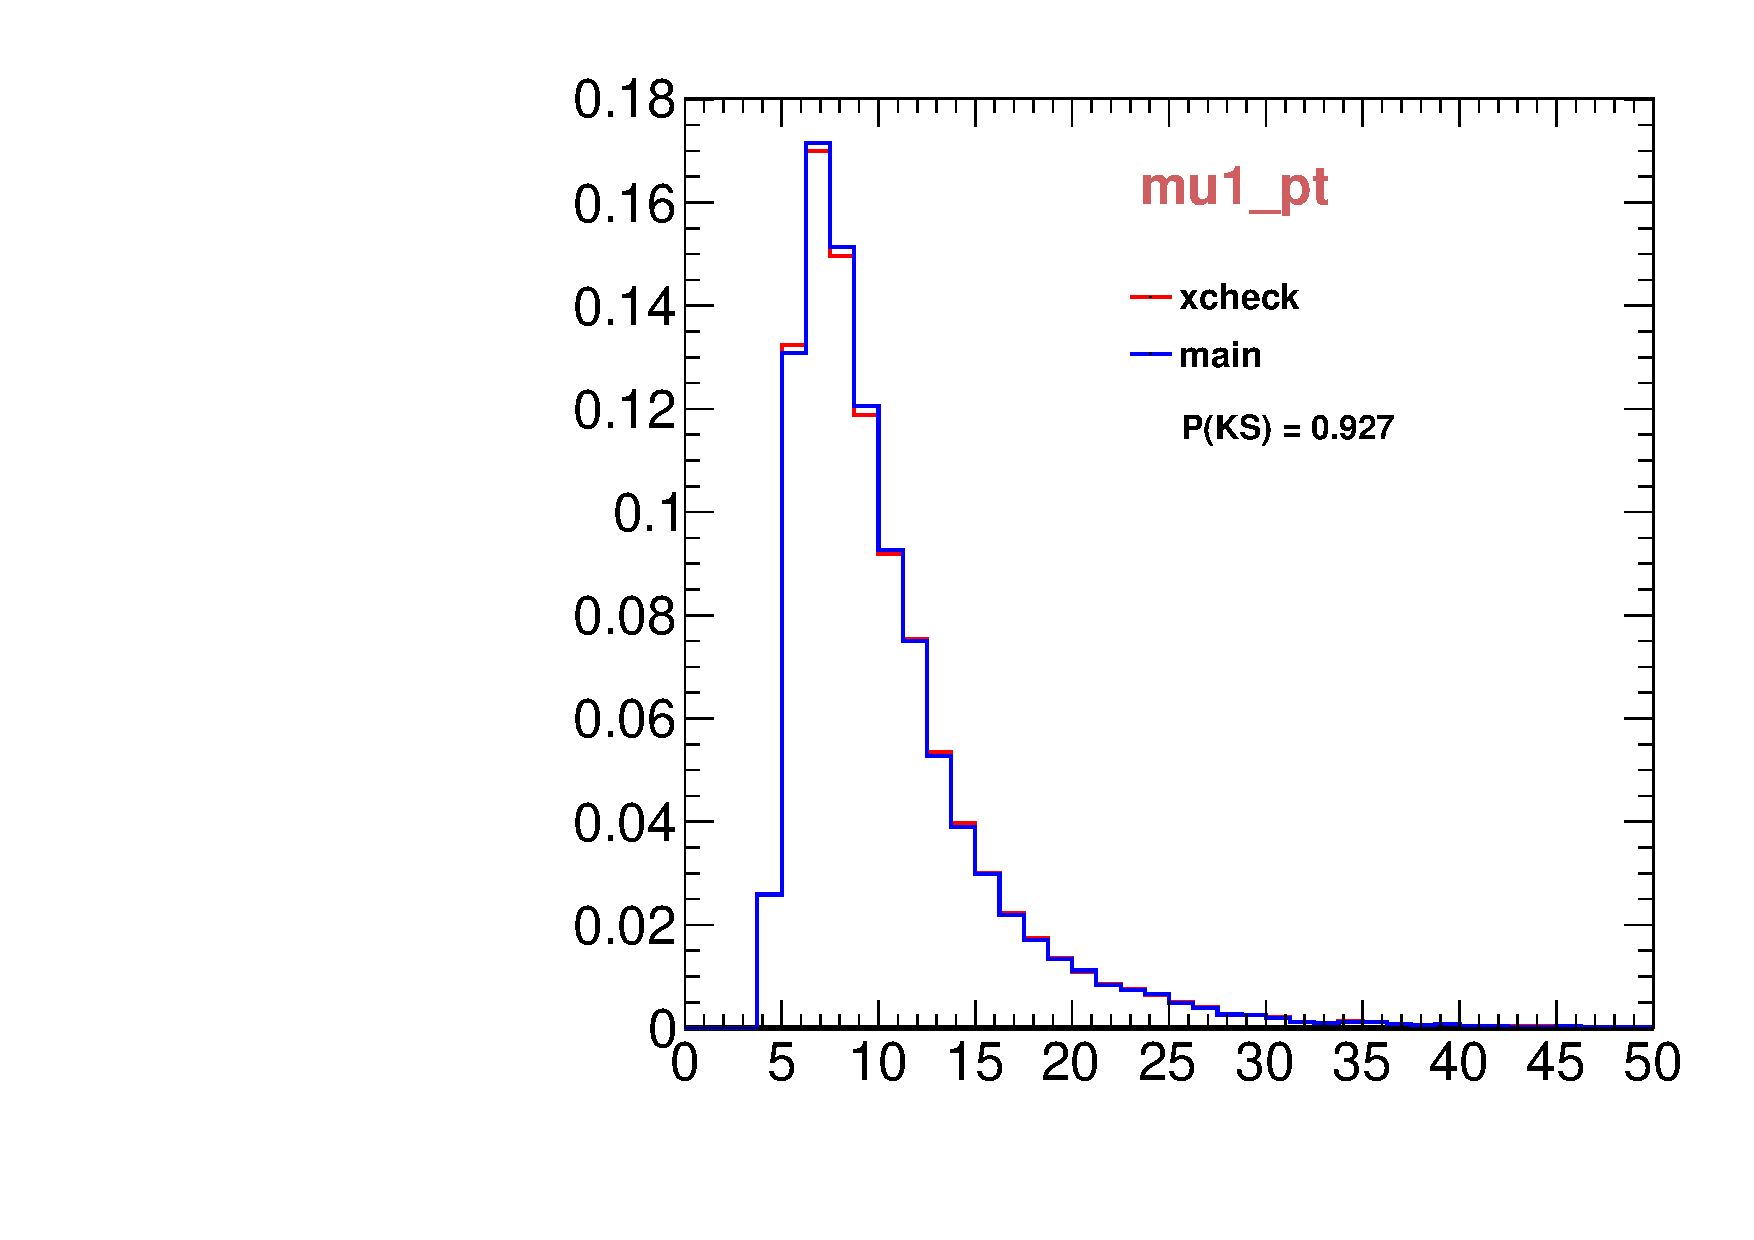
\includegraphics[width=0.3\textwidth]{Figures/VariablesComparison/MC_barrel_figs/m1pt}
  %\label{fig:MC_barrel_m1pt}
  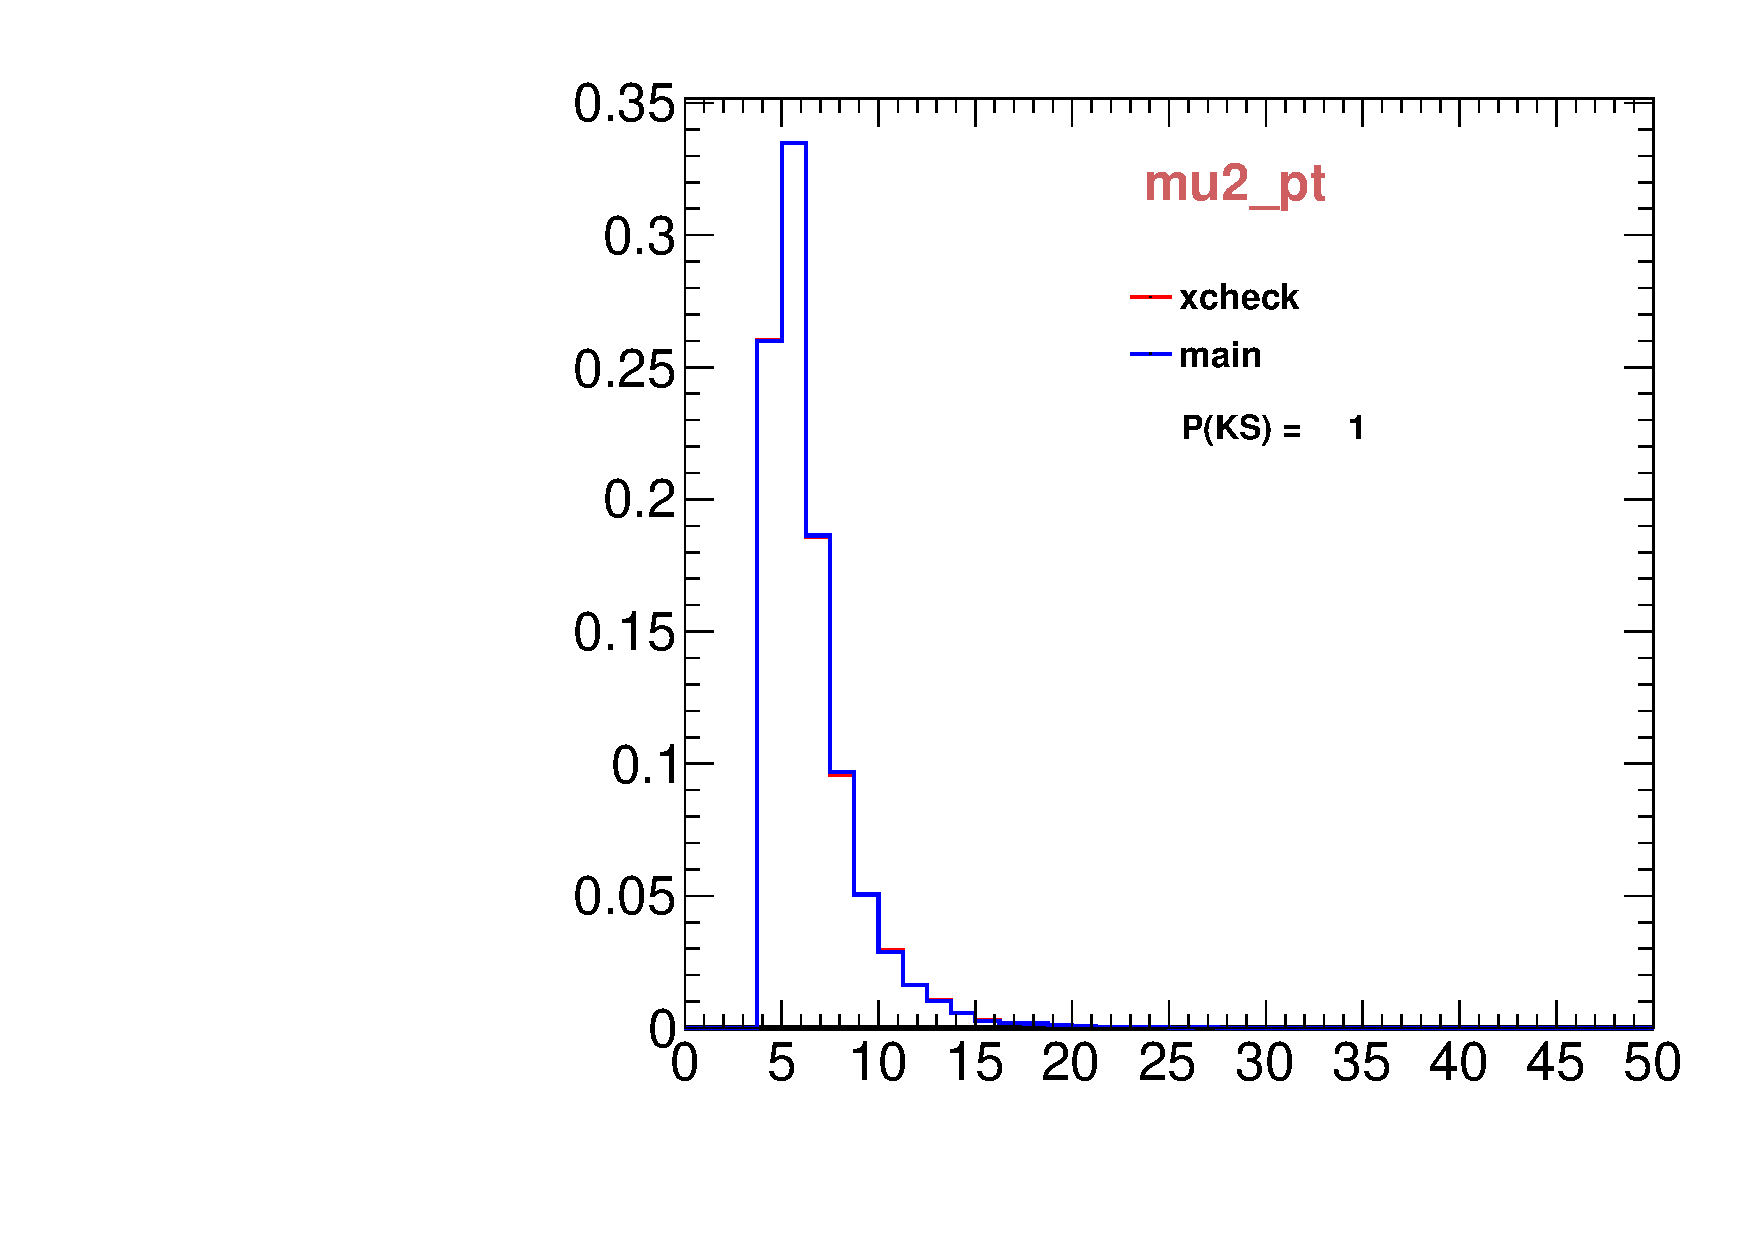
\includegraphics[width=0.3\textwidth]{Figures/VariablesComparison/MC_barrel_figs/m2pt}
  %\label{fig:MC_barrel_m2pt}
  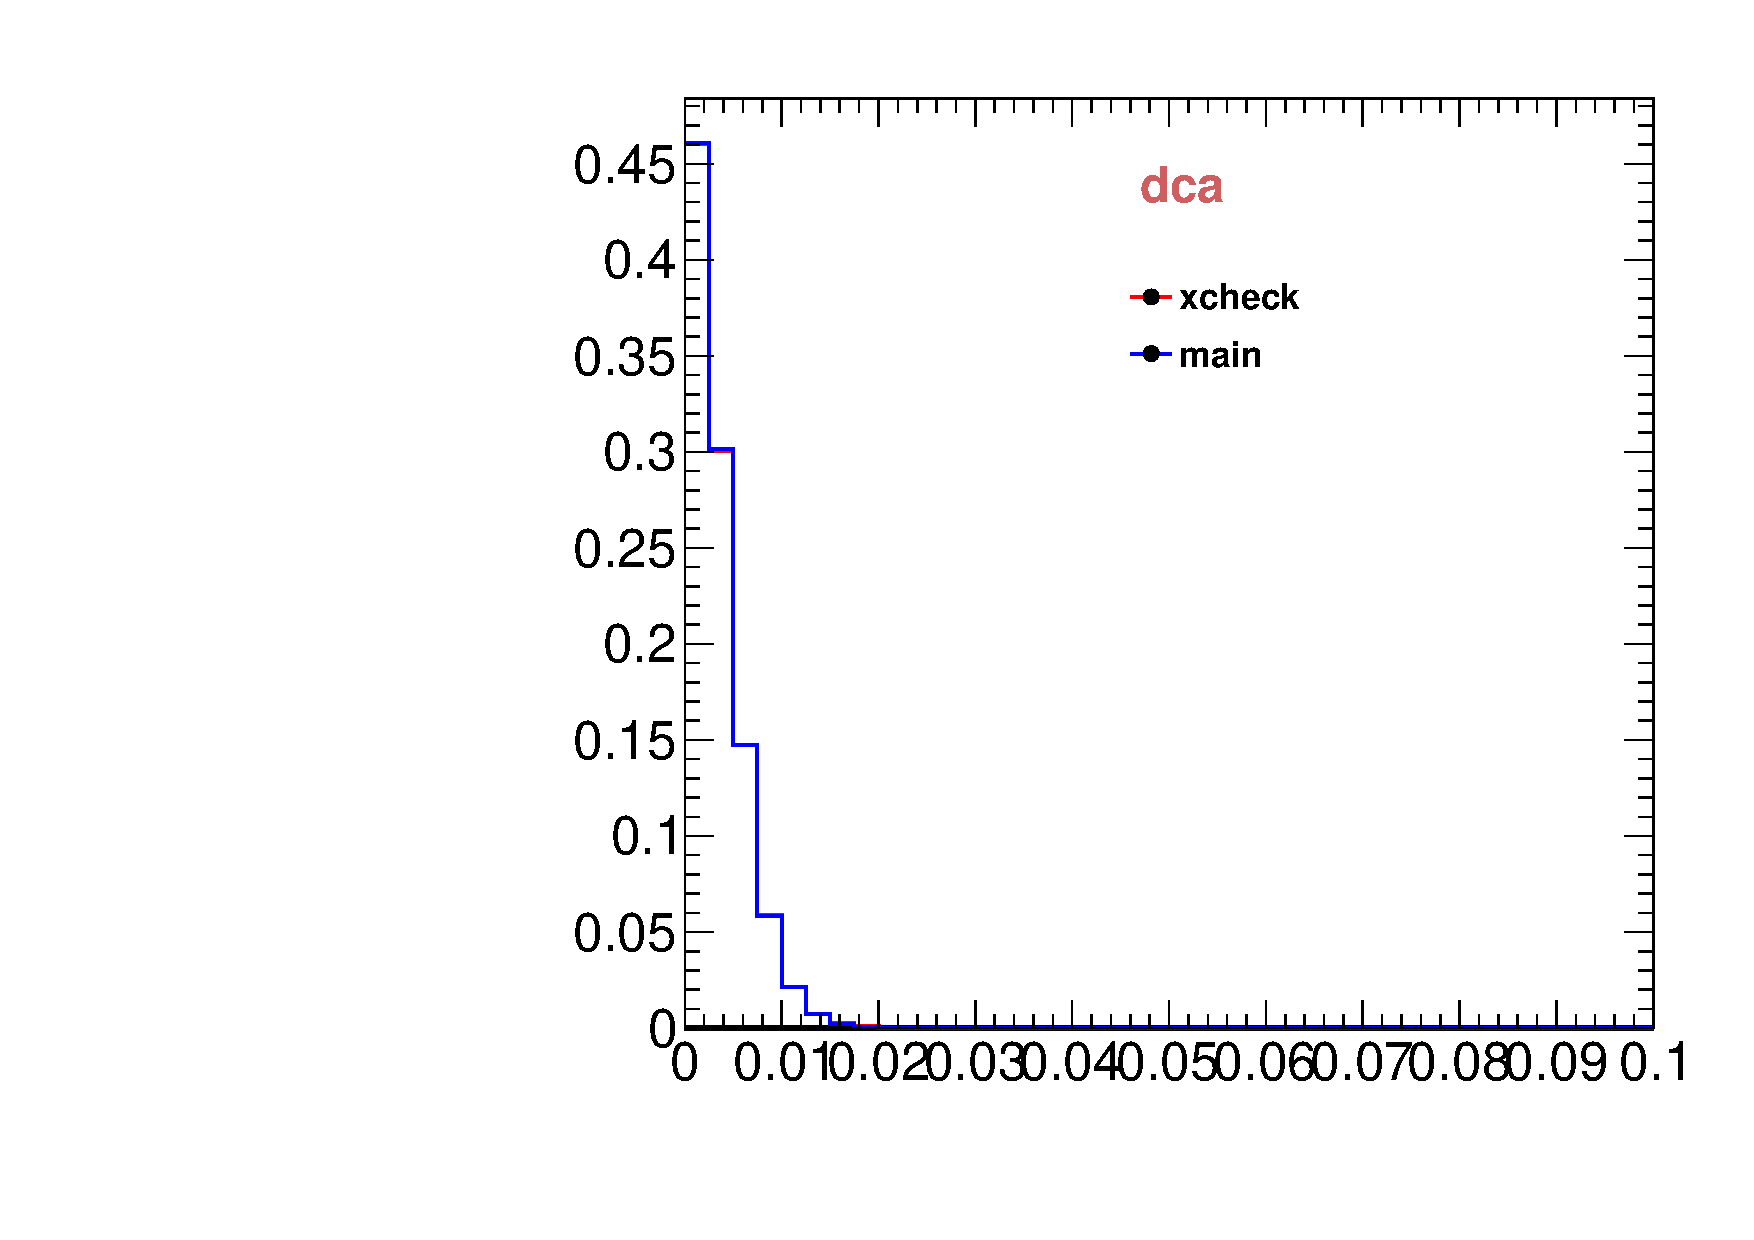
\includegraphics[width=0.3\textwidth]{Figures/VariablesComparison/MC_barrel_figs/maxdoca}
  %\label{fig:MC_barrel_maxdoca}
  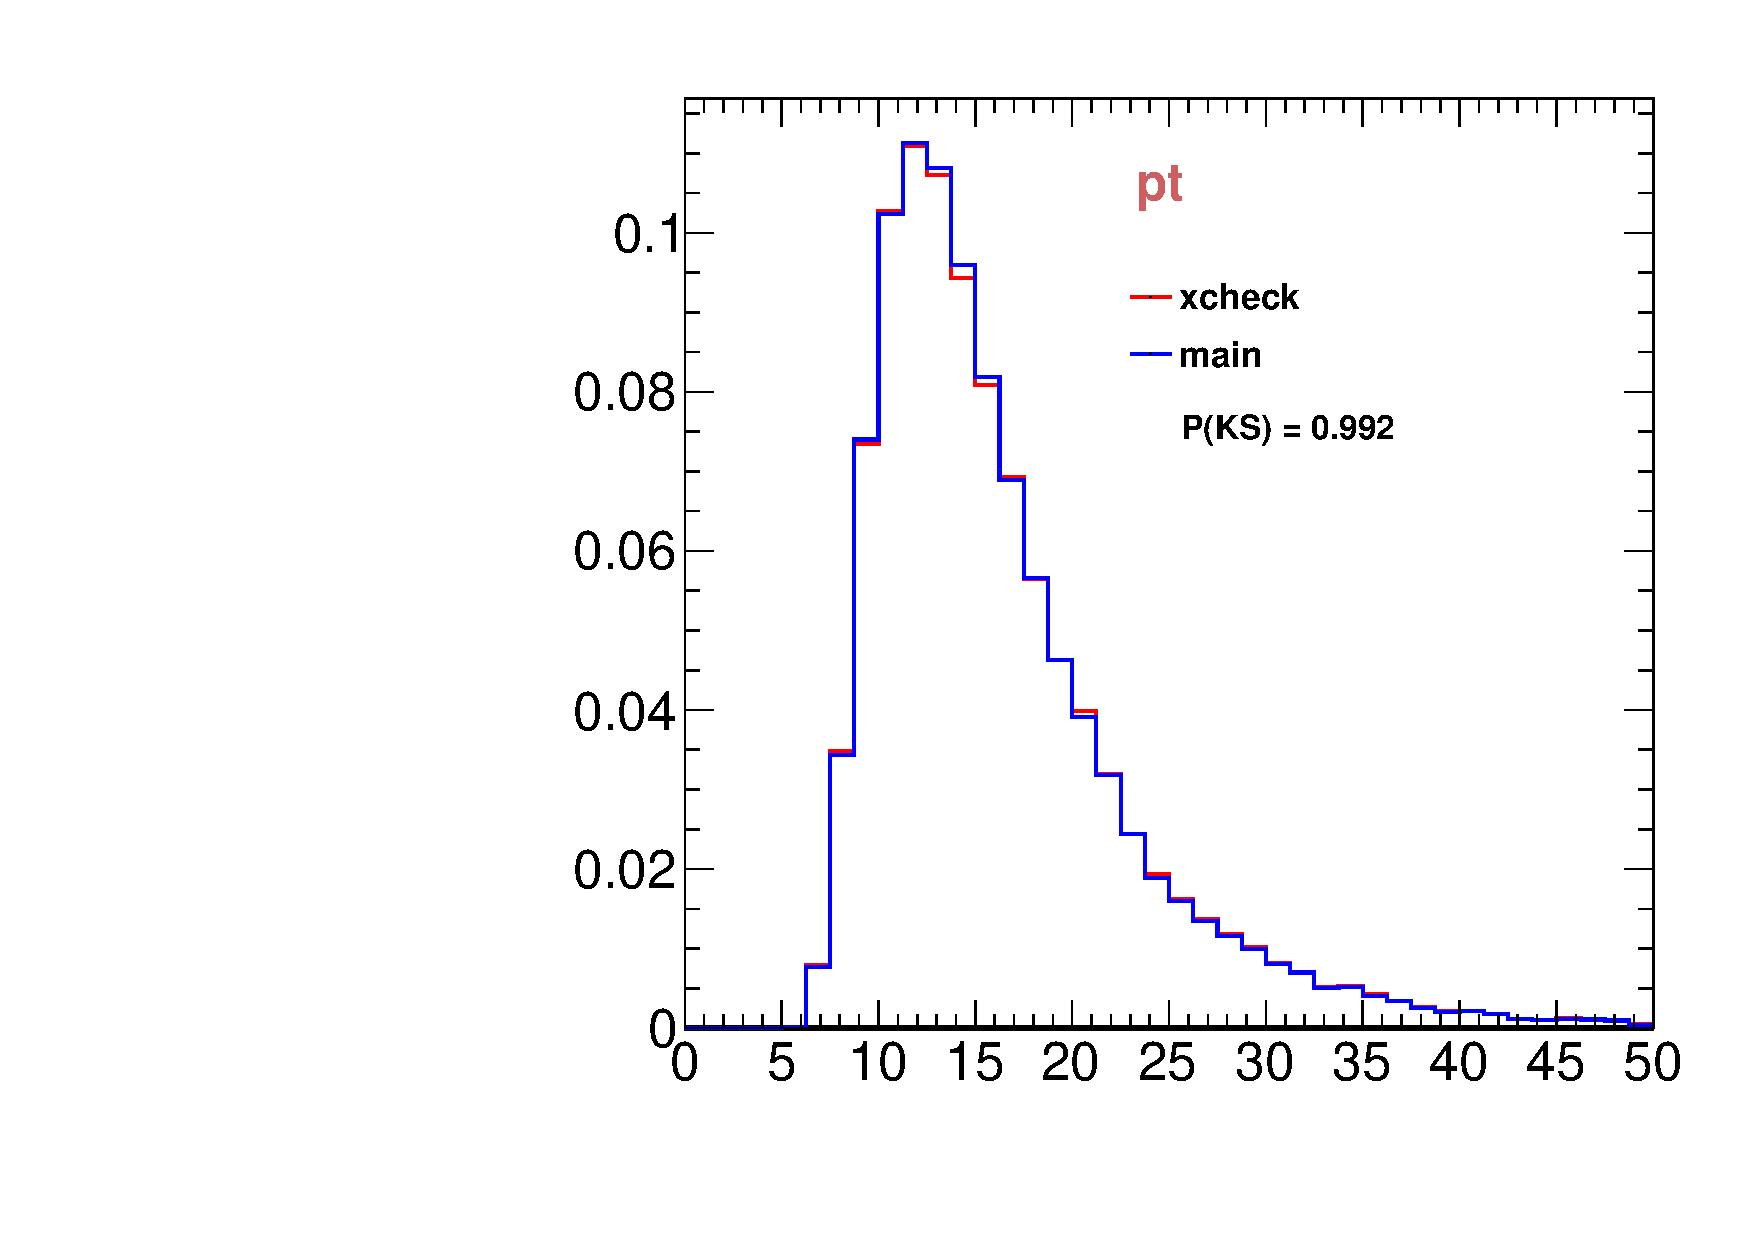
\includegraphics[width=0.3\textwidth]{Figures/VariablesComparison/MC_barrel_figs/pt}
  %\label{fig:MC_barrel_pt}
  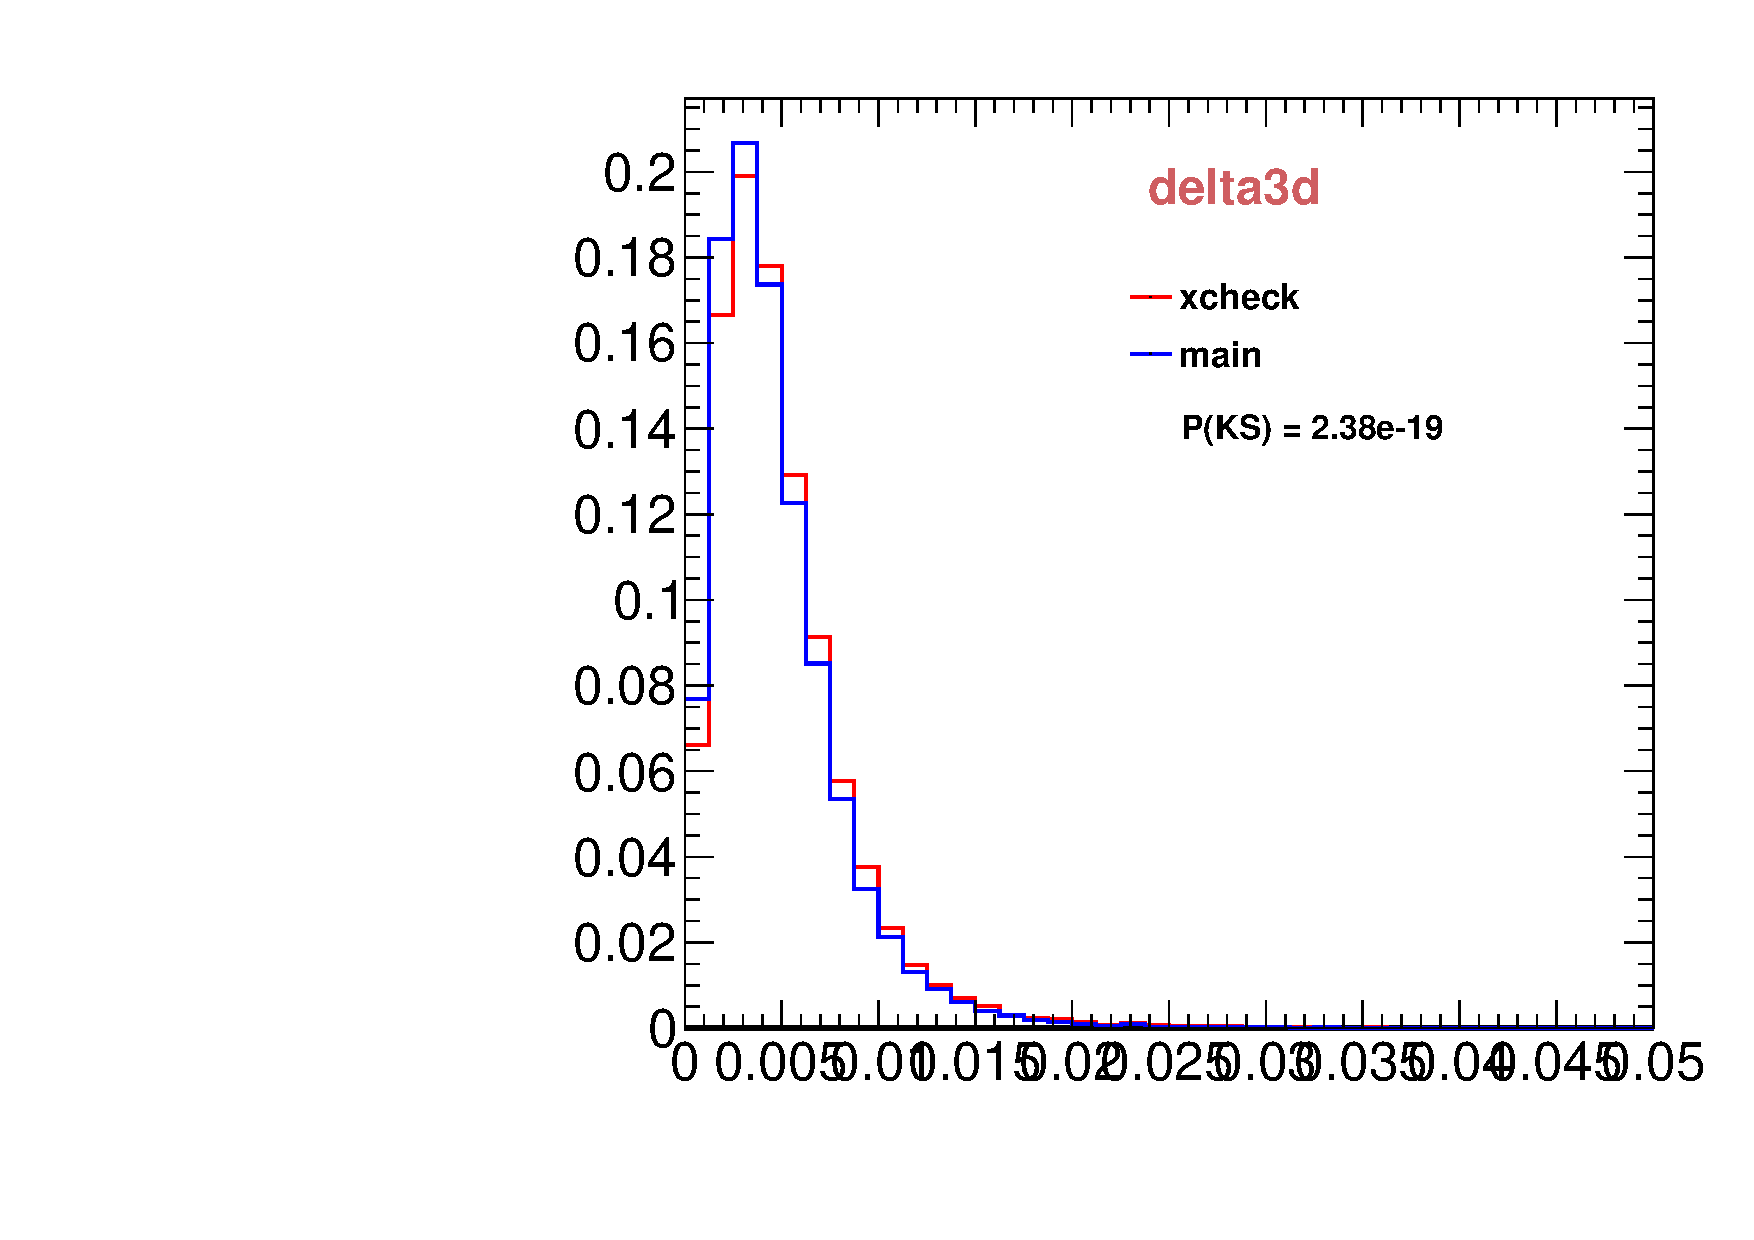
\includegraphics[width=0.3\textwidth]{Figures/VariablesComparison/MC_barrel_figs/pvip}
  %\label{fig:MC_barrel_pvip}
  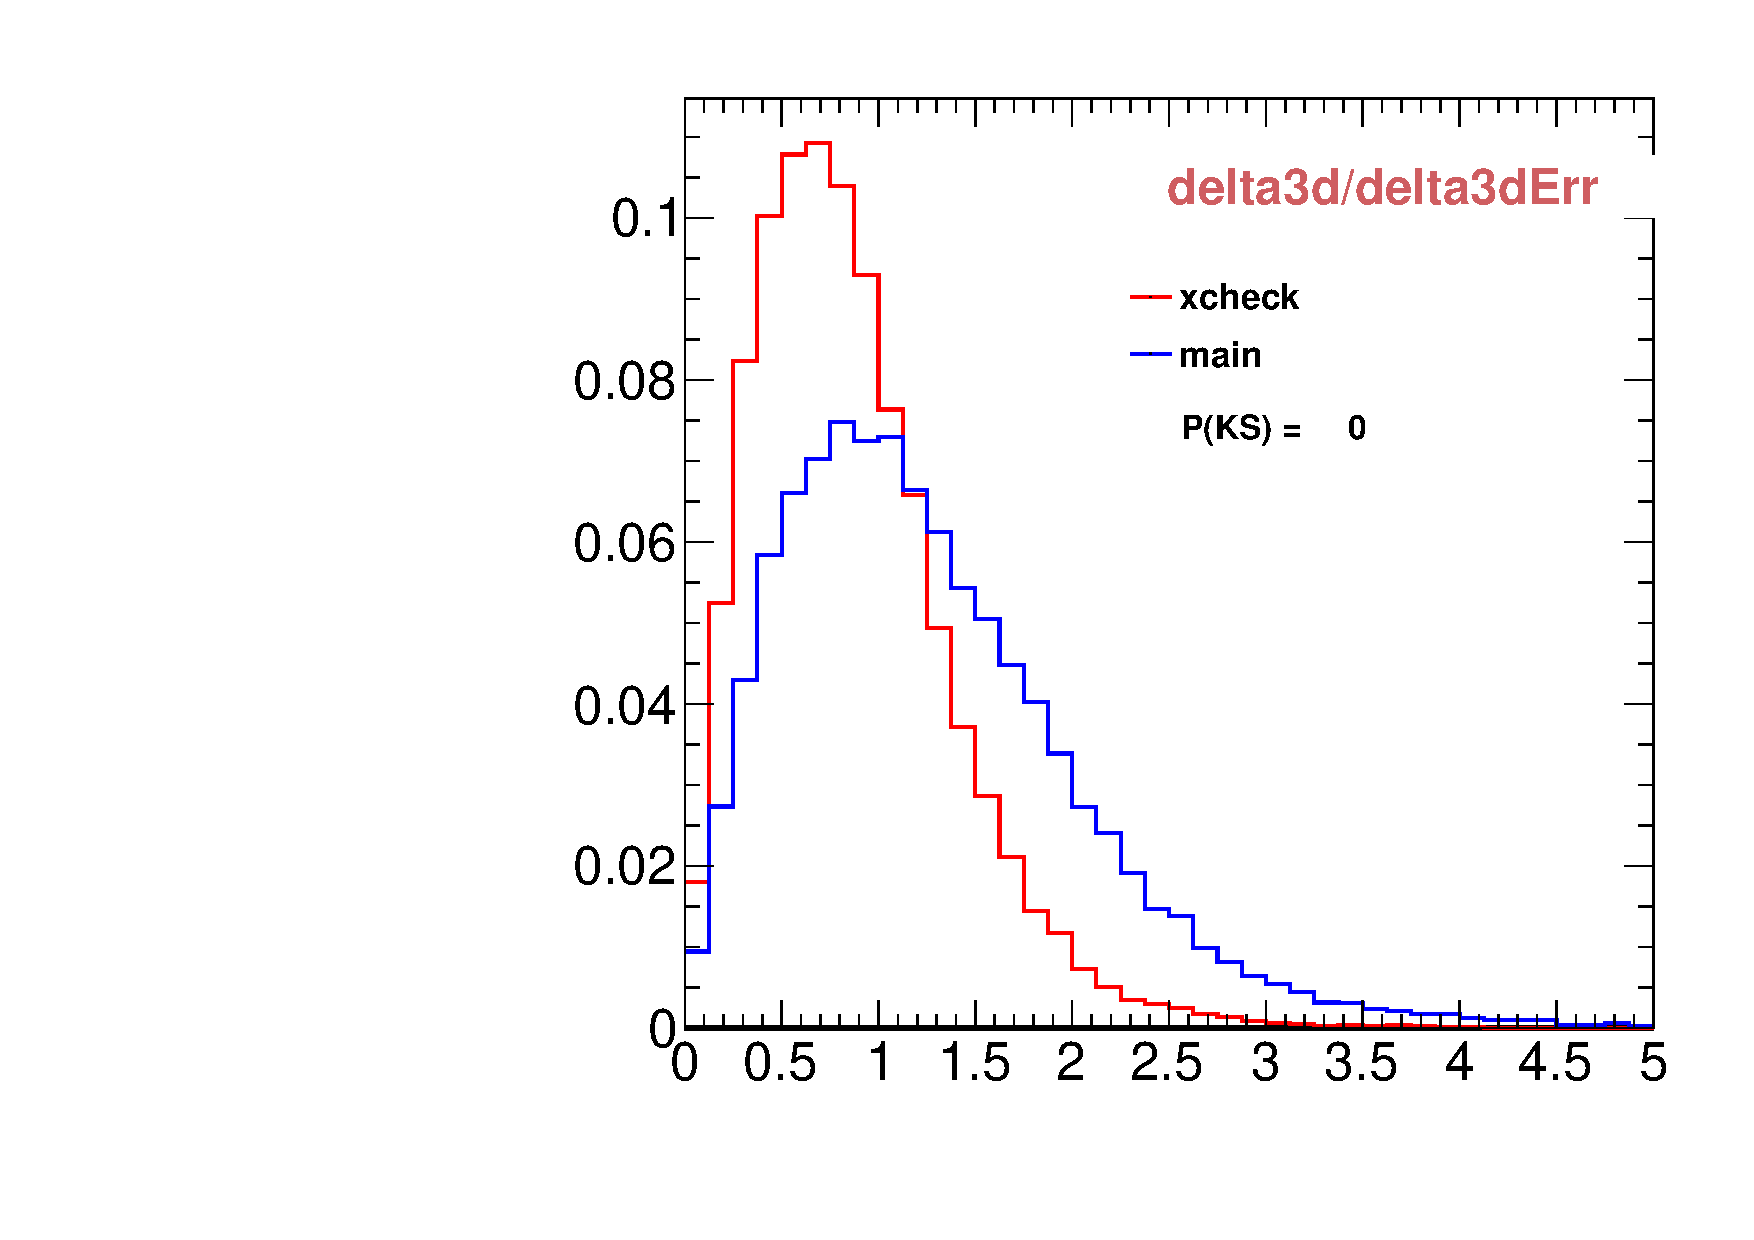
\includegraphics[width=0.3\textwidth]{Figures/VariablesComparison/MC_barrel_figs/pvips}
  %\label{fig:MC_barrel_pvips}
  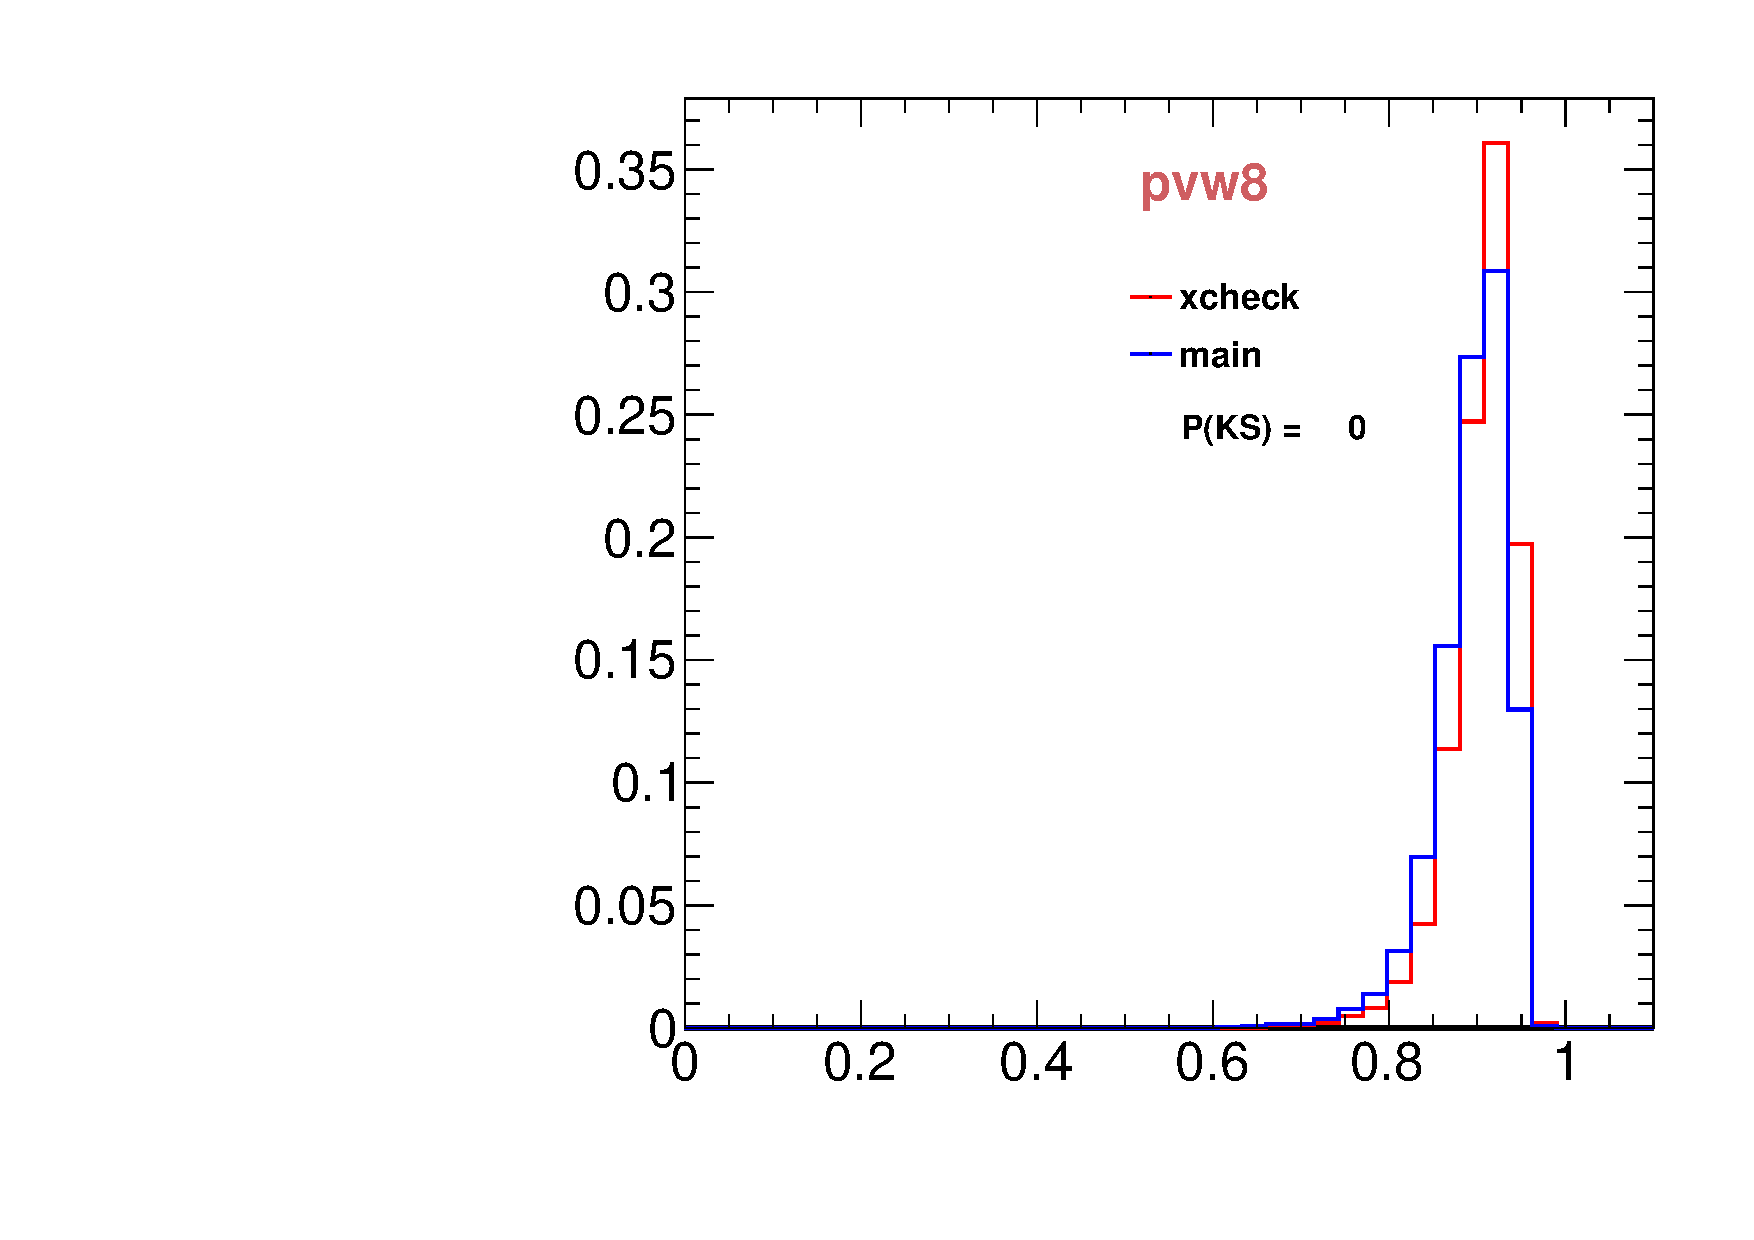
\includegraphics[width=0.3\textwidth]{Figures/VariablesComparison/MC_barrel_figs/pvw8}
  %\label{fig:MC_barrel_pvw8}
  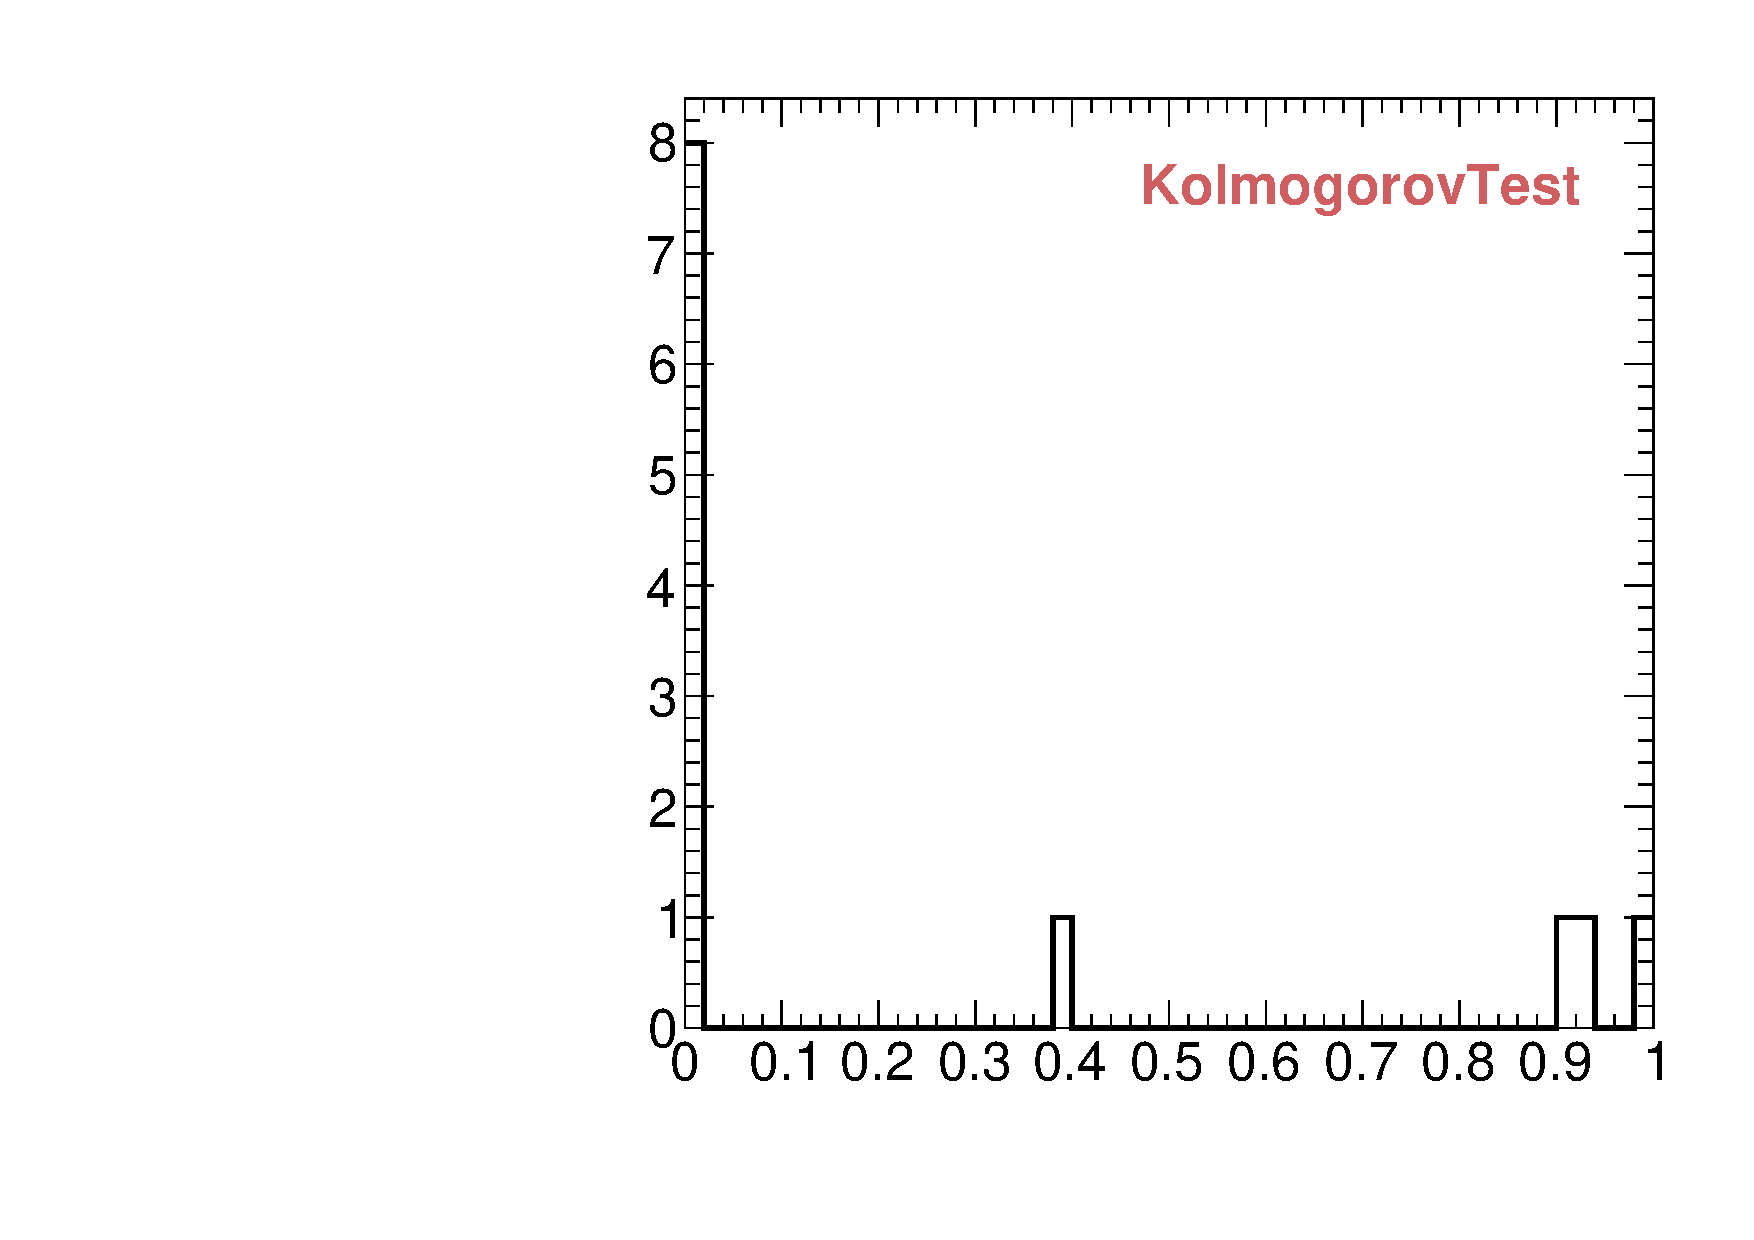
\includegraphics[width=0.3\textwidth]{Figures/VariablesComparison/MC_barrel_figs/KS}
  %\label{fig:MC_barrel_KS}
  \caption{Variable comparisons between the main analysis and the cross-check analysis. Part I: MC barrel.}
  \label{fig:MC_barrel_figs}
\end{figure}

\begin{figure}
  \centering
  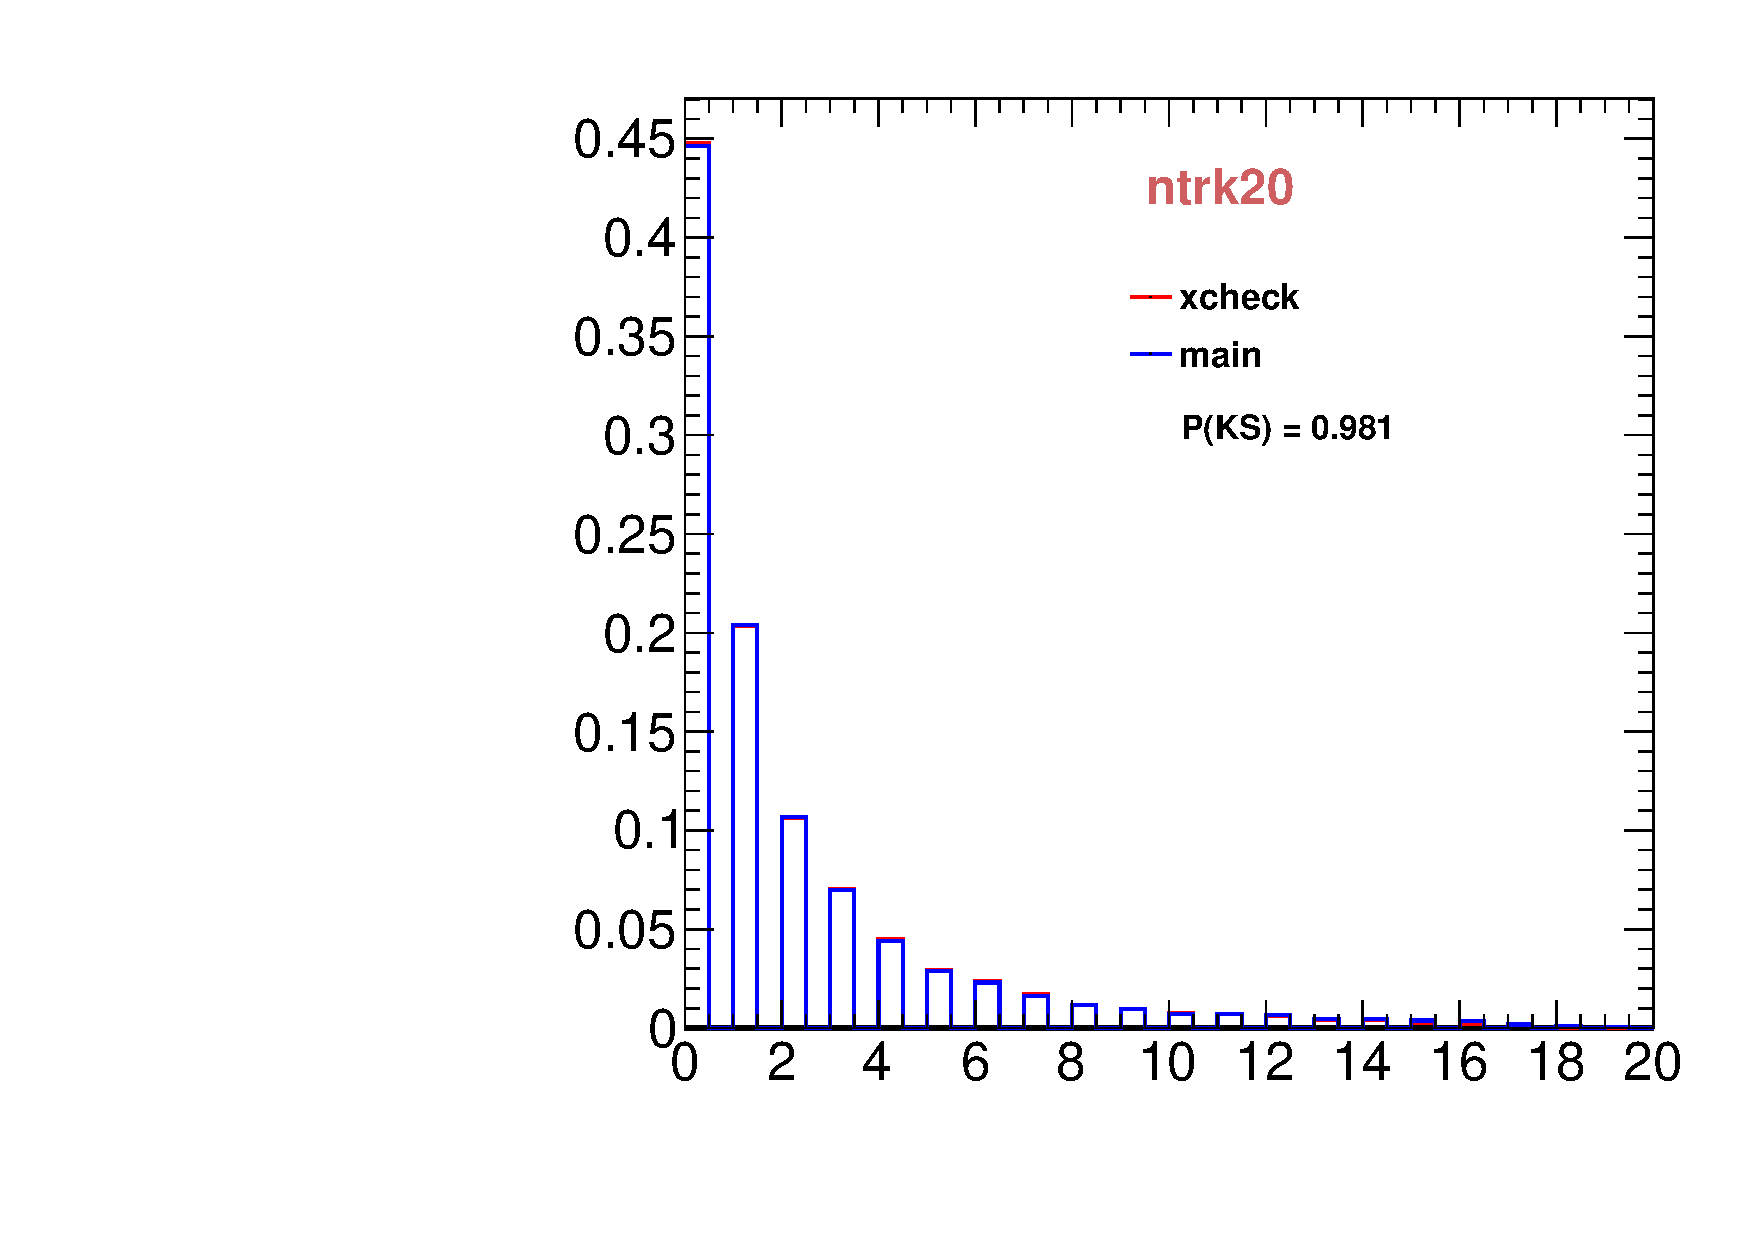
\includegraphics[width=0.3\textwidth]{Figures/VariablesComparison/MC_endcaps_figs/closetrk}
  %\label{fig:MC_endcaps_closetrk}
  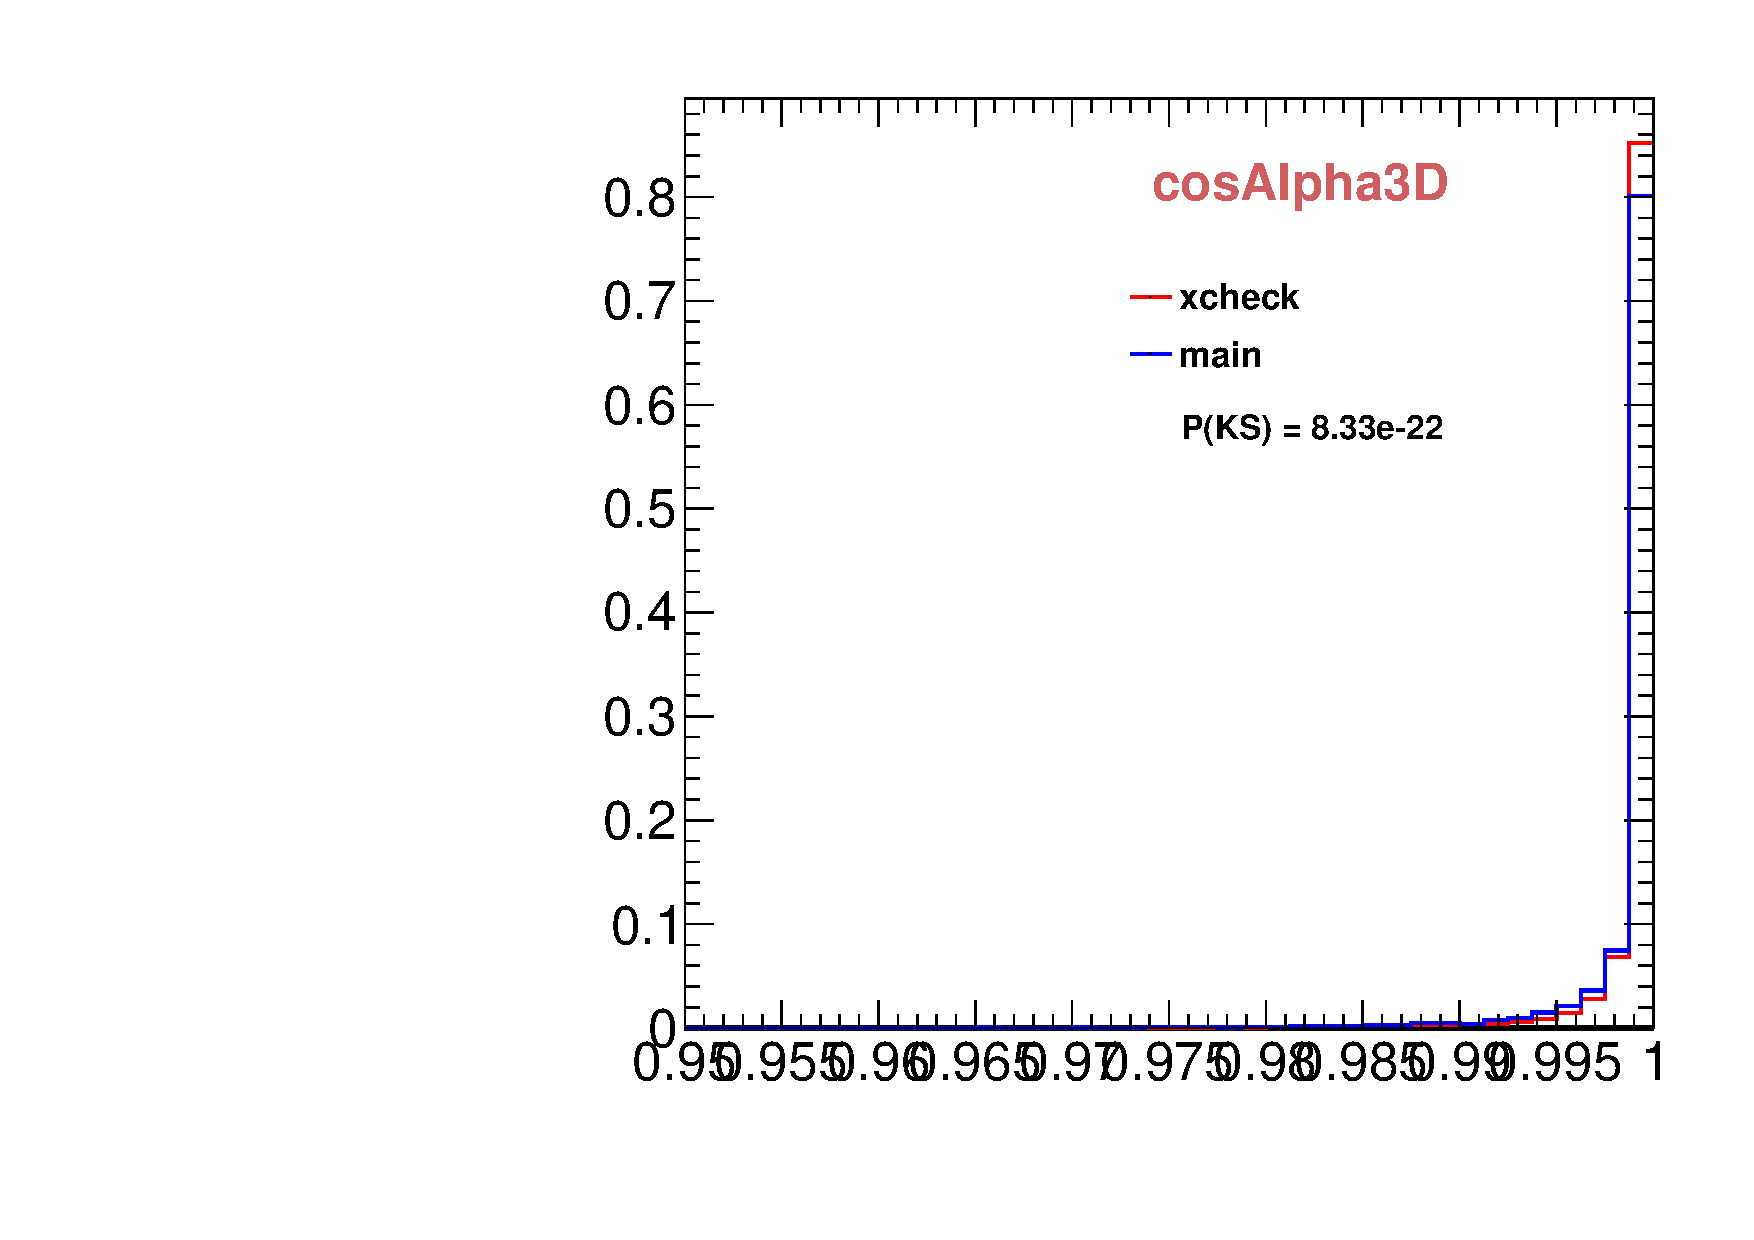
\includegraphics[width=0.3\textwidth]{Figures/VariablesComparison/MC_endcaps_figs/cosa}
  %\label{fig:MC_endcaps_cosa}
  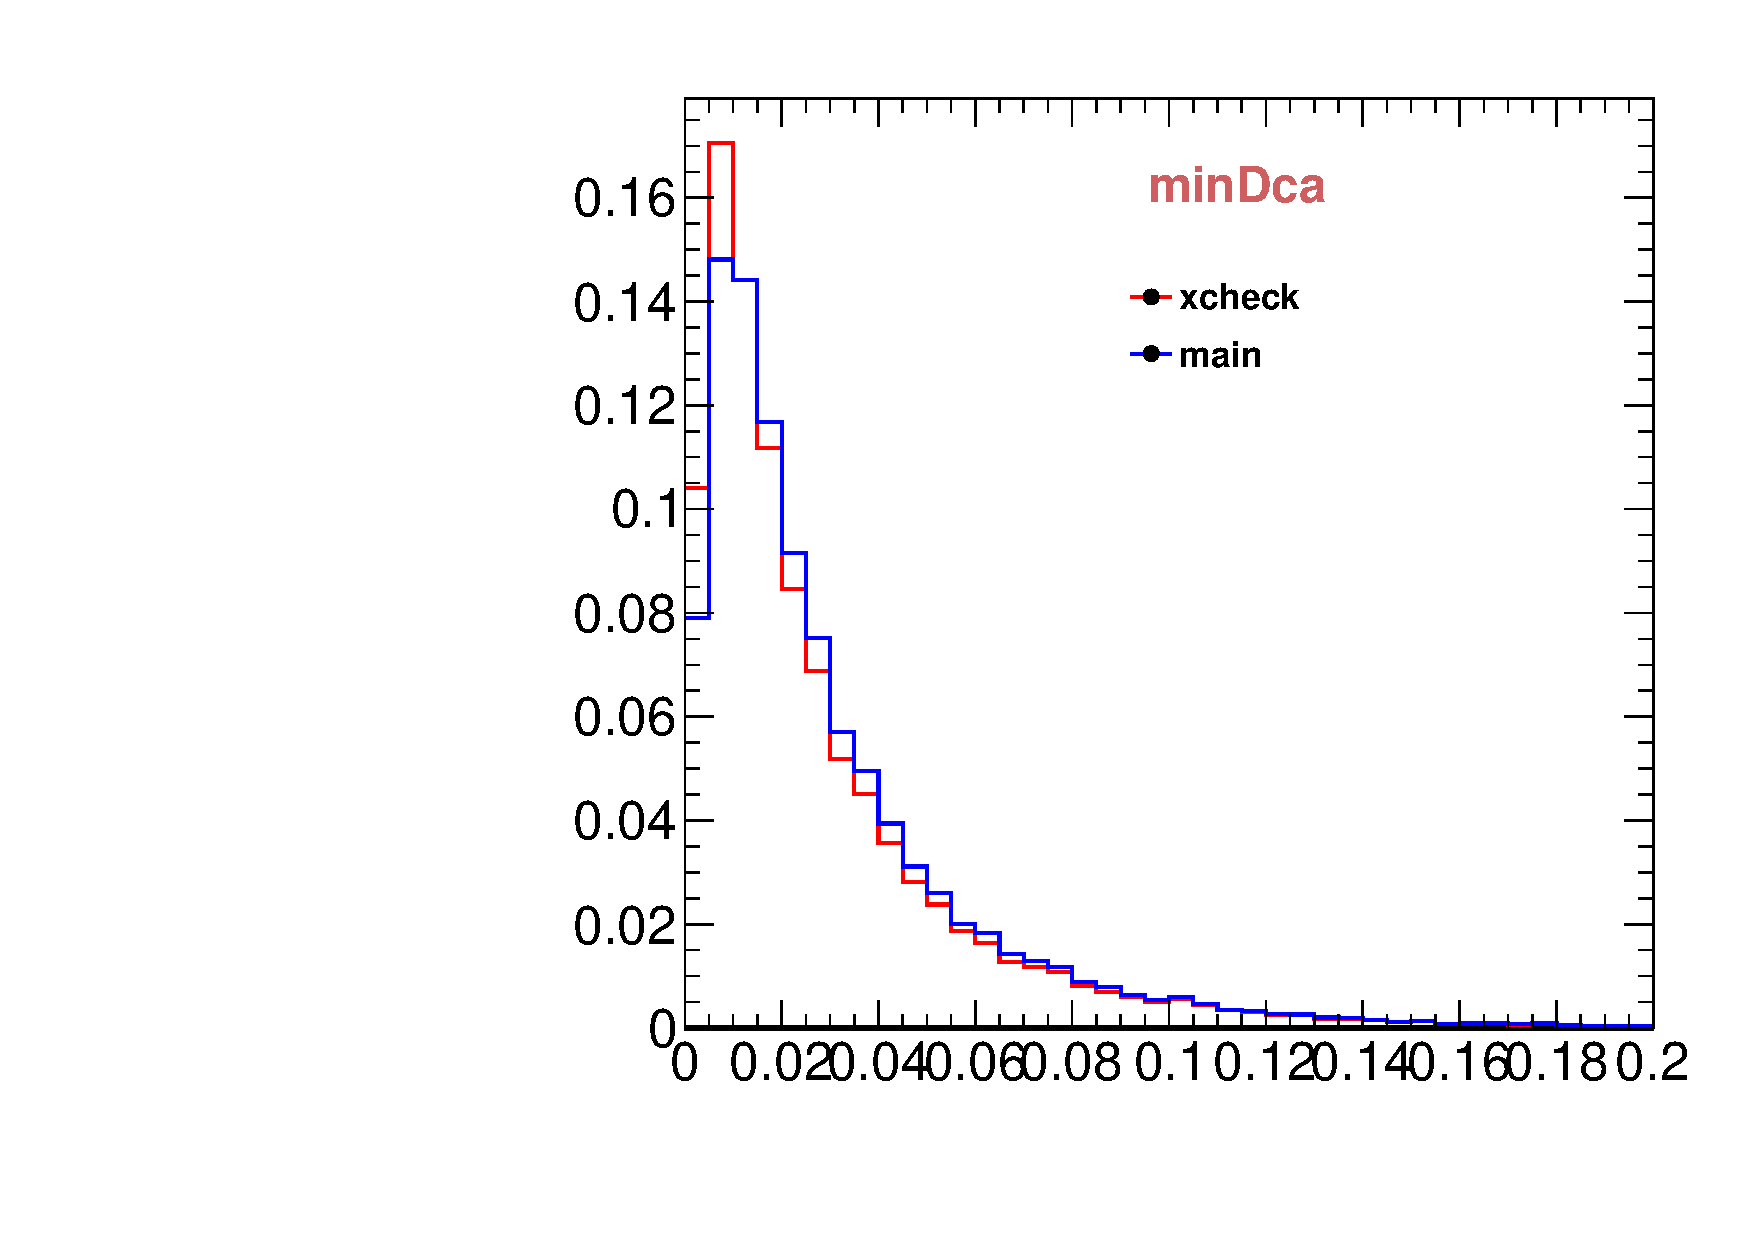
\includegraphics[width=0.3\textwidth]{Figures/VariablesComparison/MC_endcaps_figs/docatrk}
  %\label{fig:MC_endcaps_docatrk}
  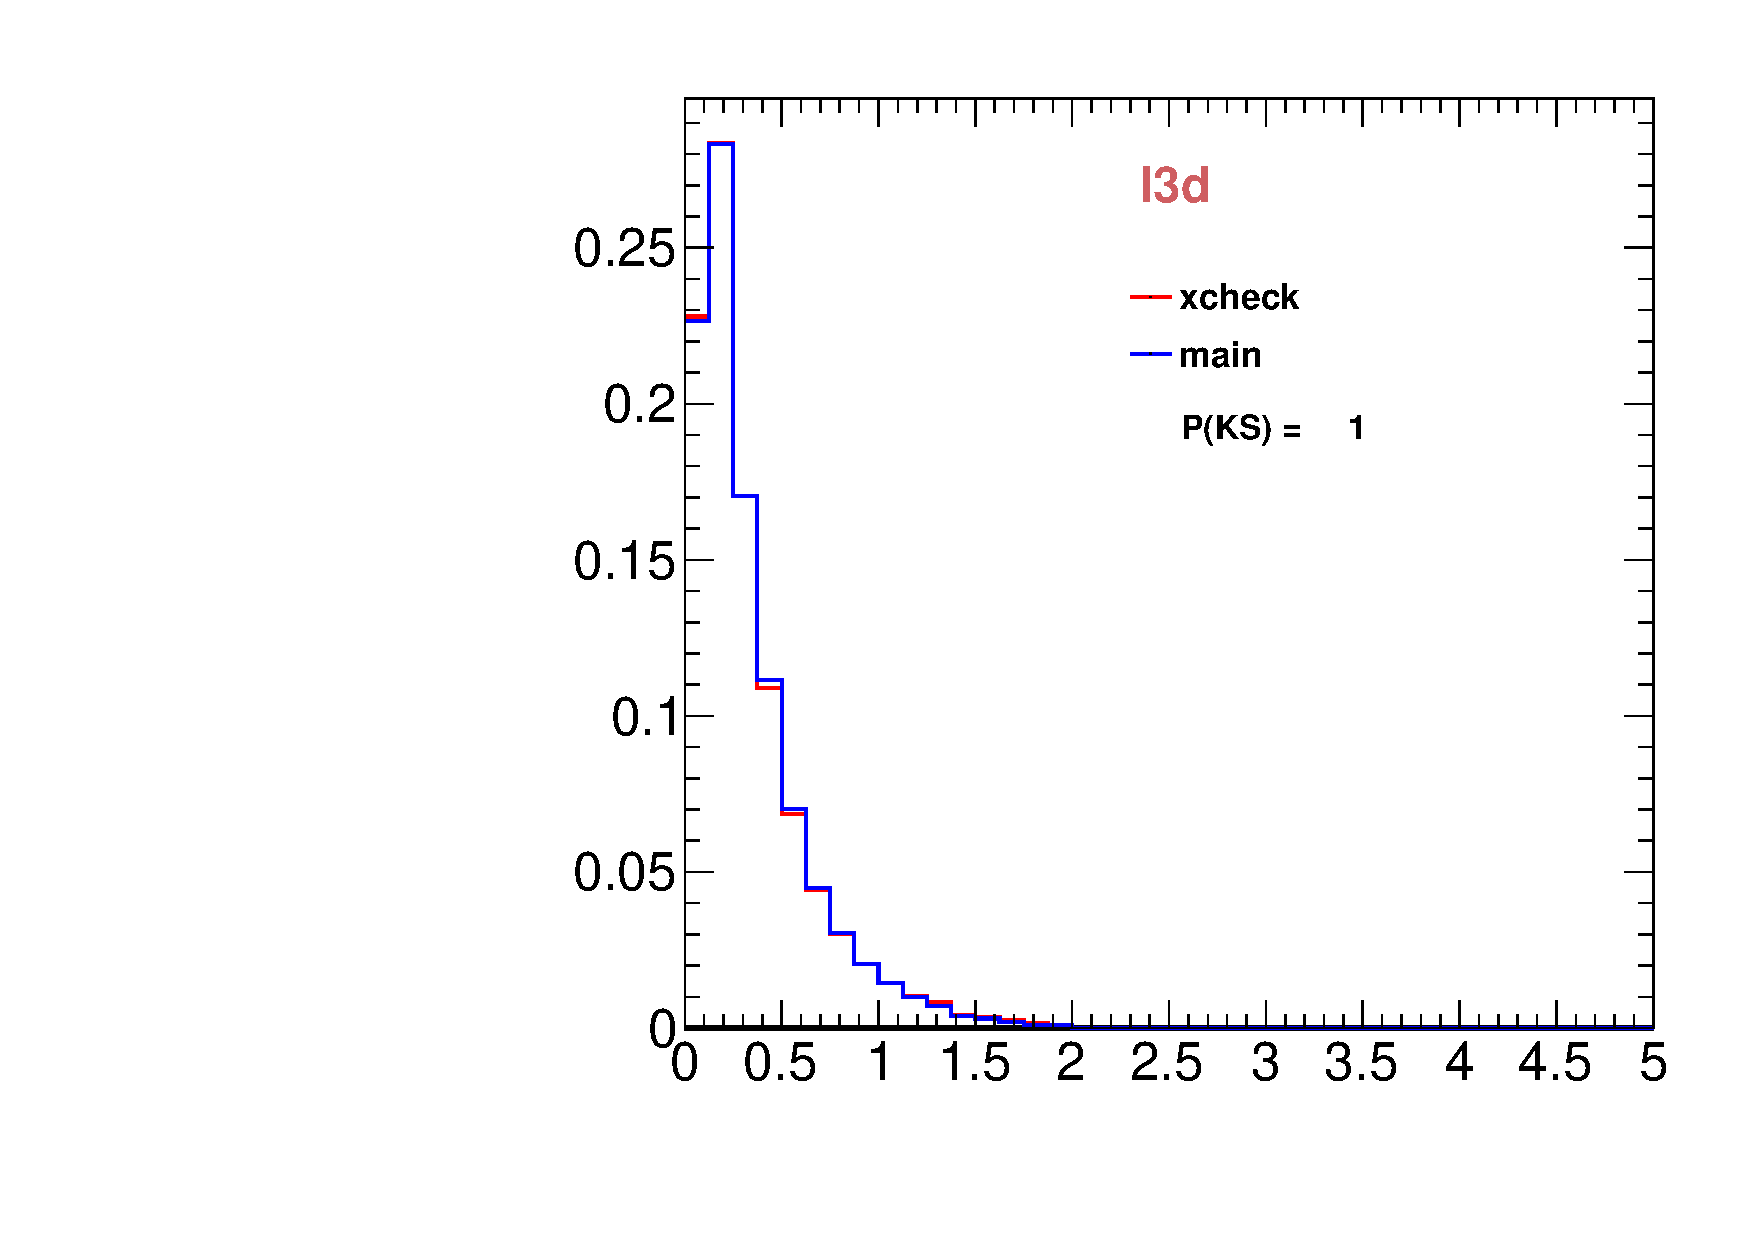
\includegraphics[width=0.3\textwidth]{Figures/VariablesComparison/MC_endcaps_figs/fl3d}
  %\label{fig:MC_endcaps_fl3d}
  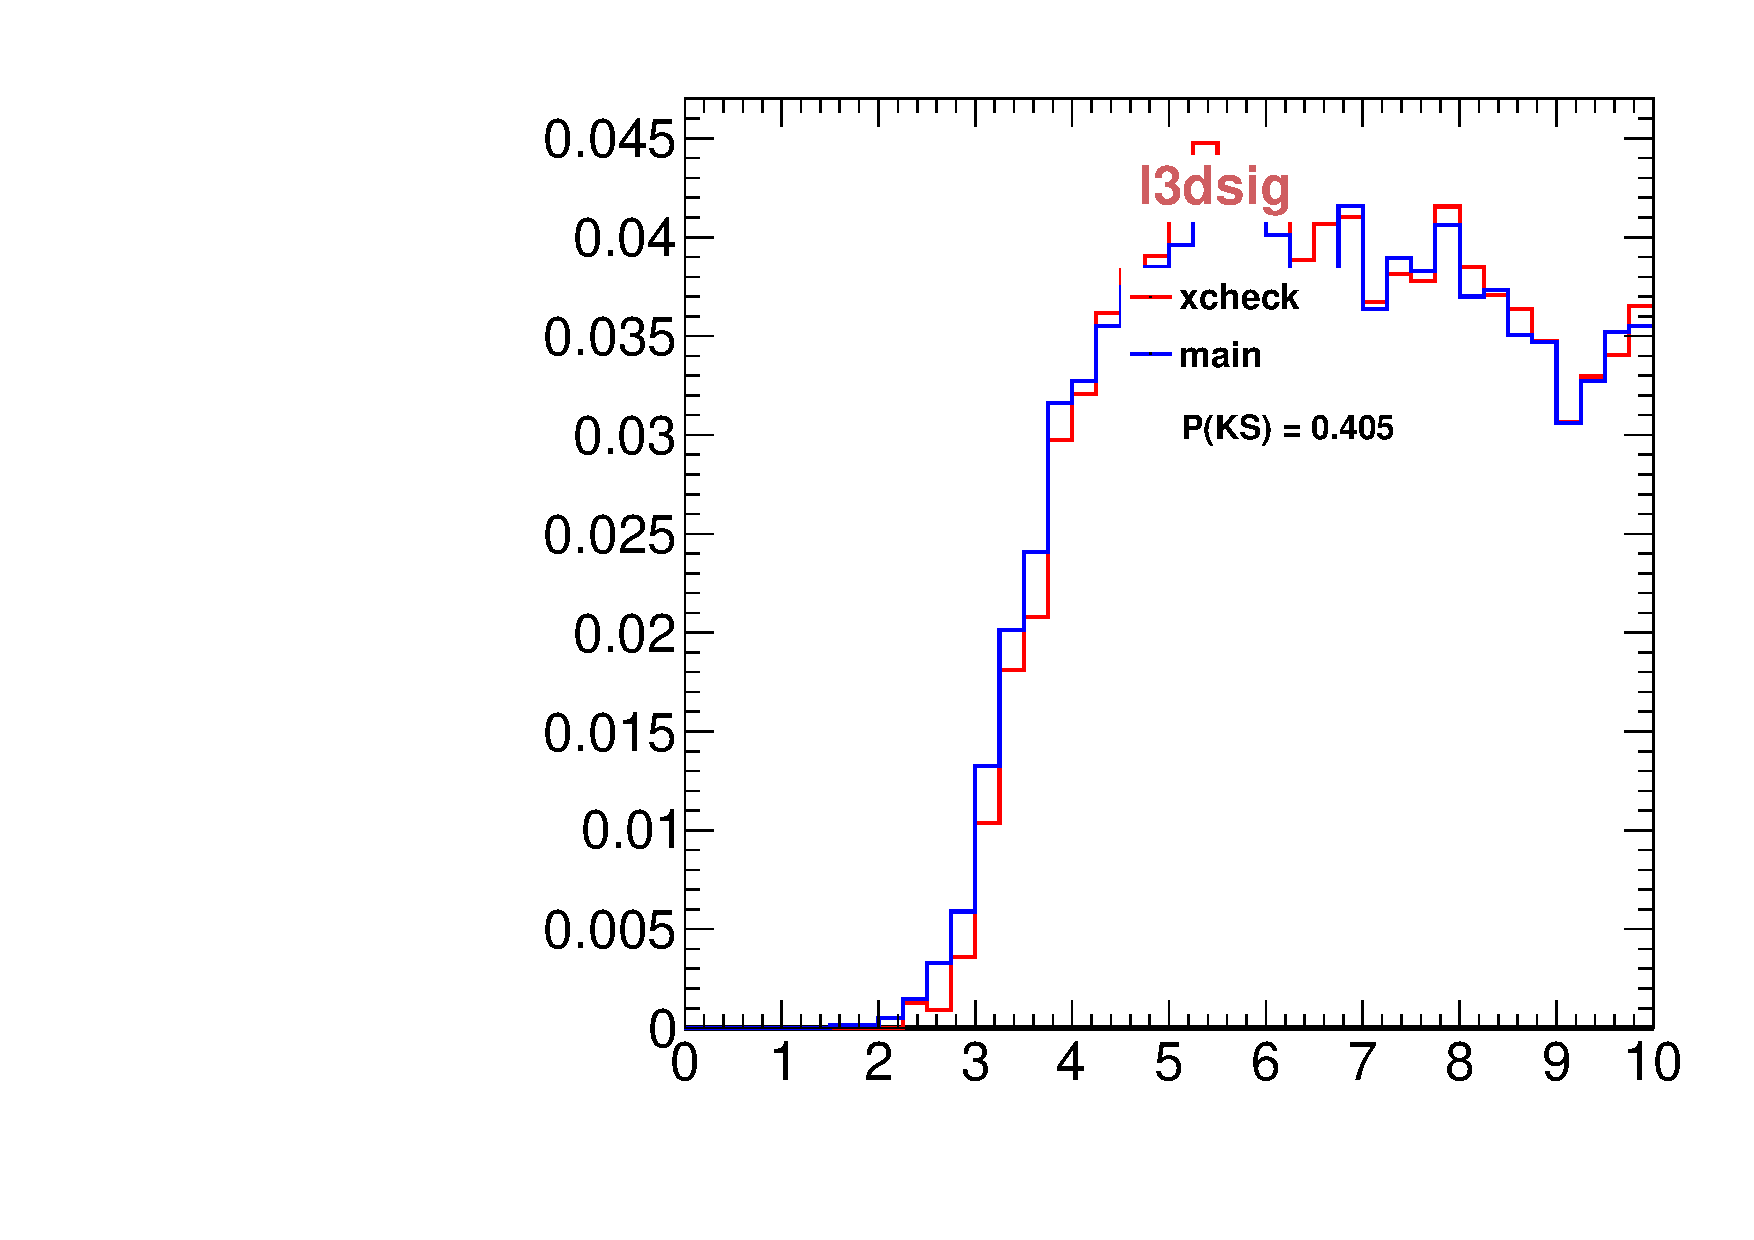
\includegraphics[width=0.3\textwidth]{Figures/VariablesComparison/MC_endcaps_figs/fls3d}
  %\label{fig:MC_endcaps_fls3d}
  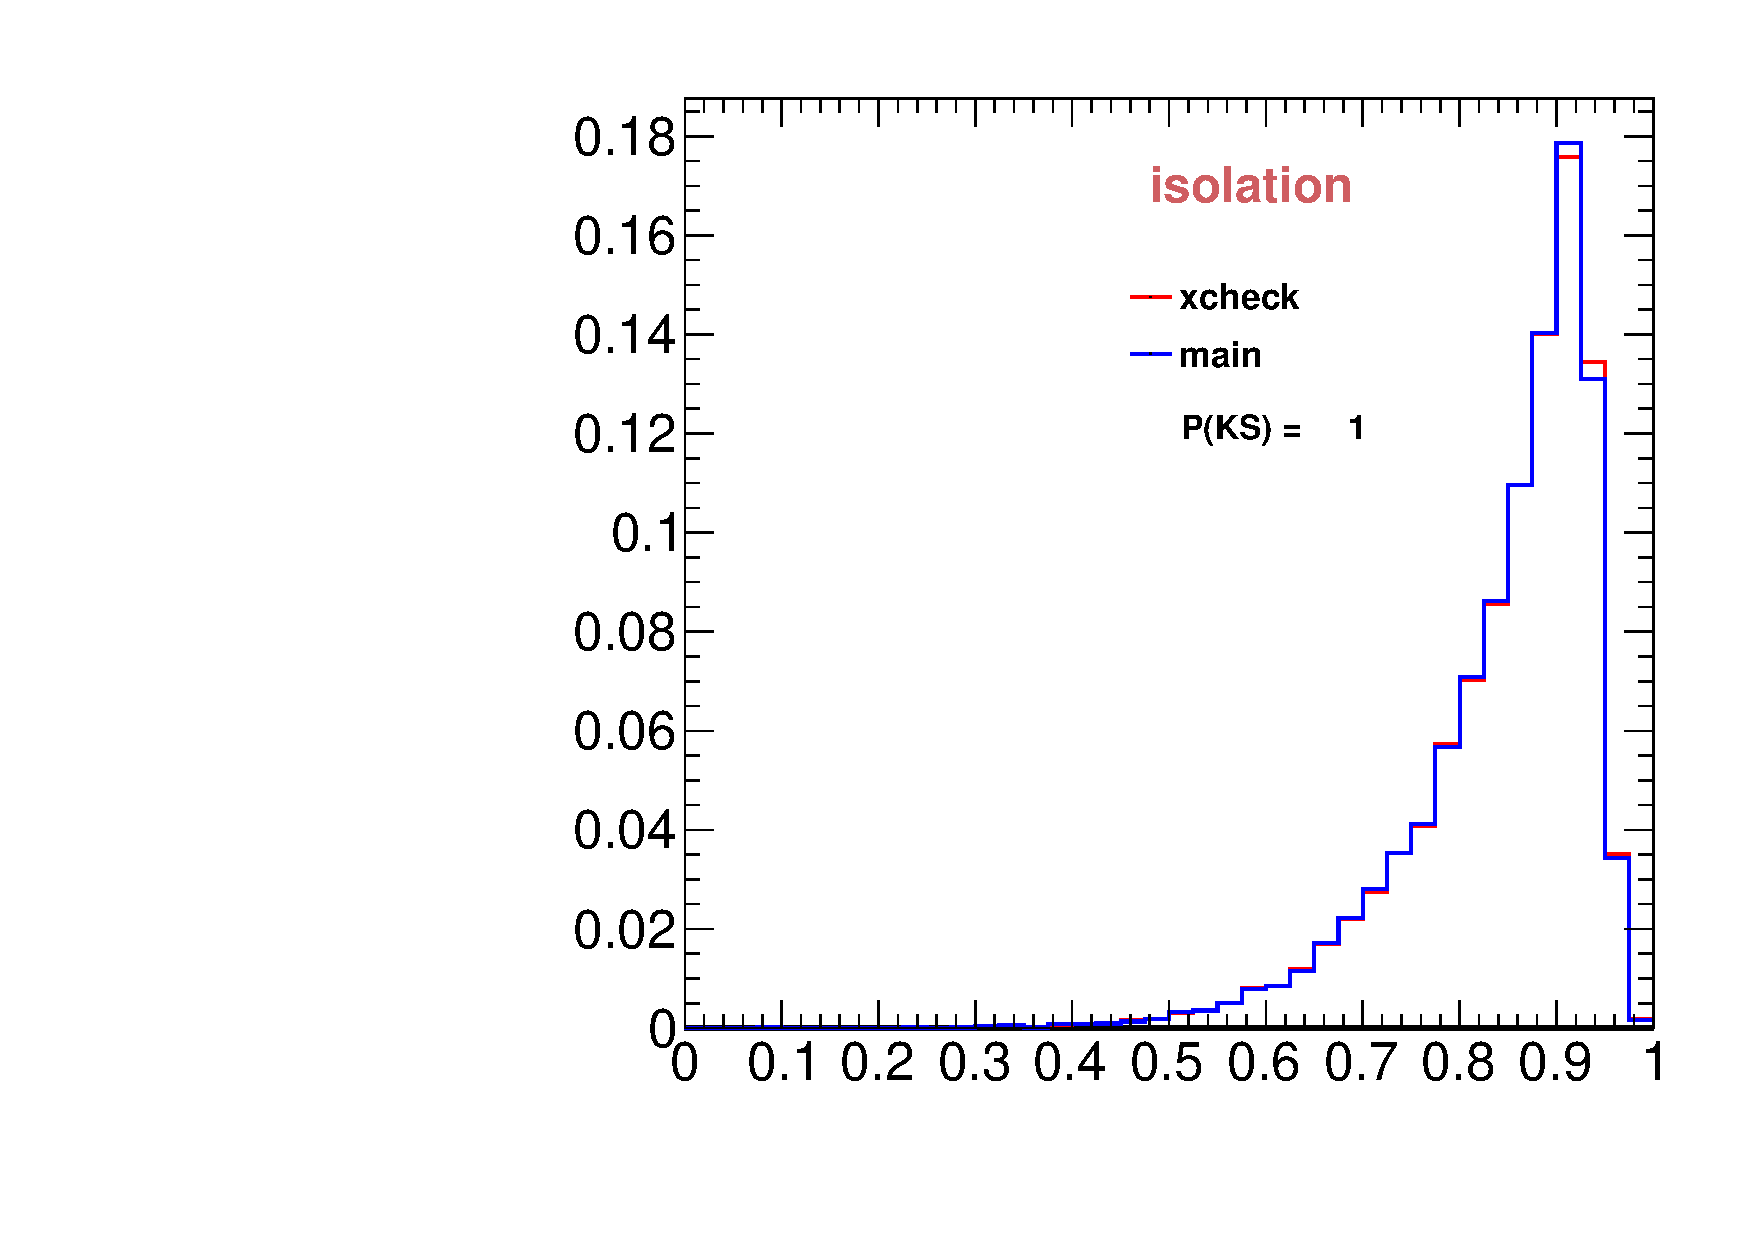
\includegraphics[width=0.3\textwidth]{Figures/VariablesComparison/MC_endcaps_figs/iso}
  %\label{fig:MC_endcaps_iso}
  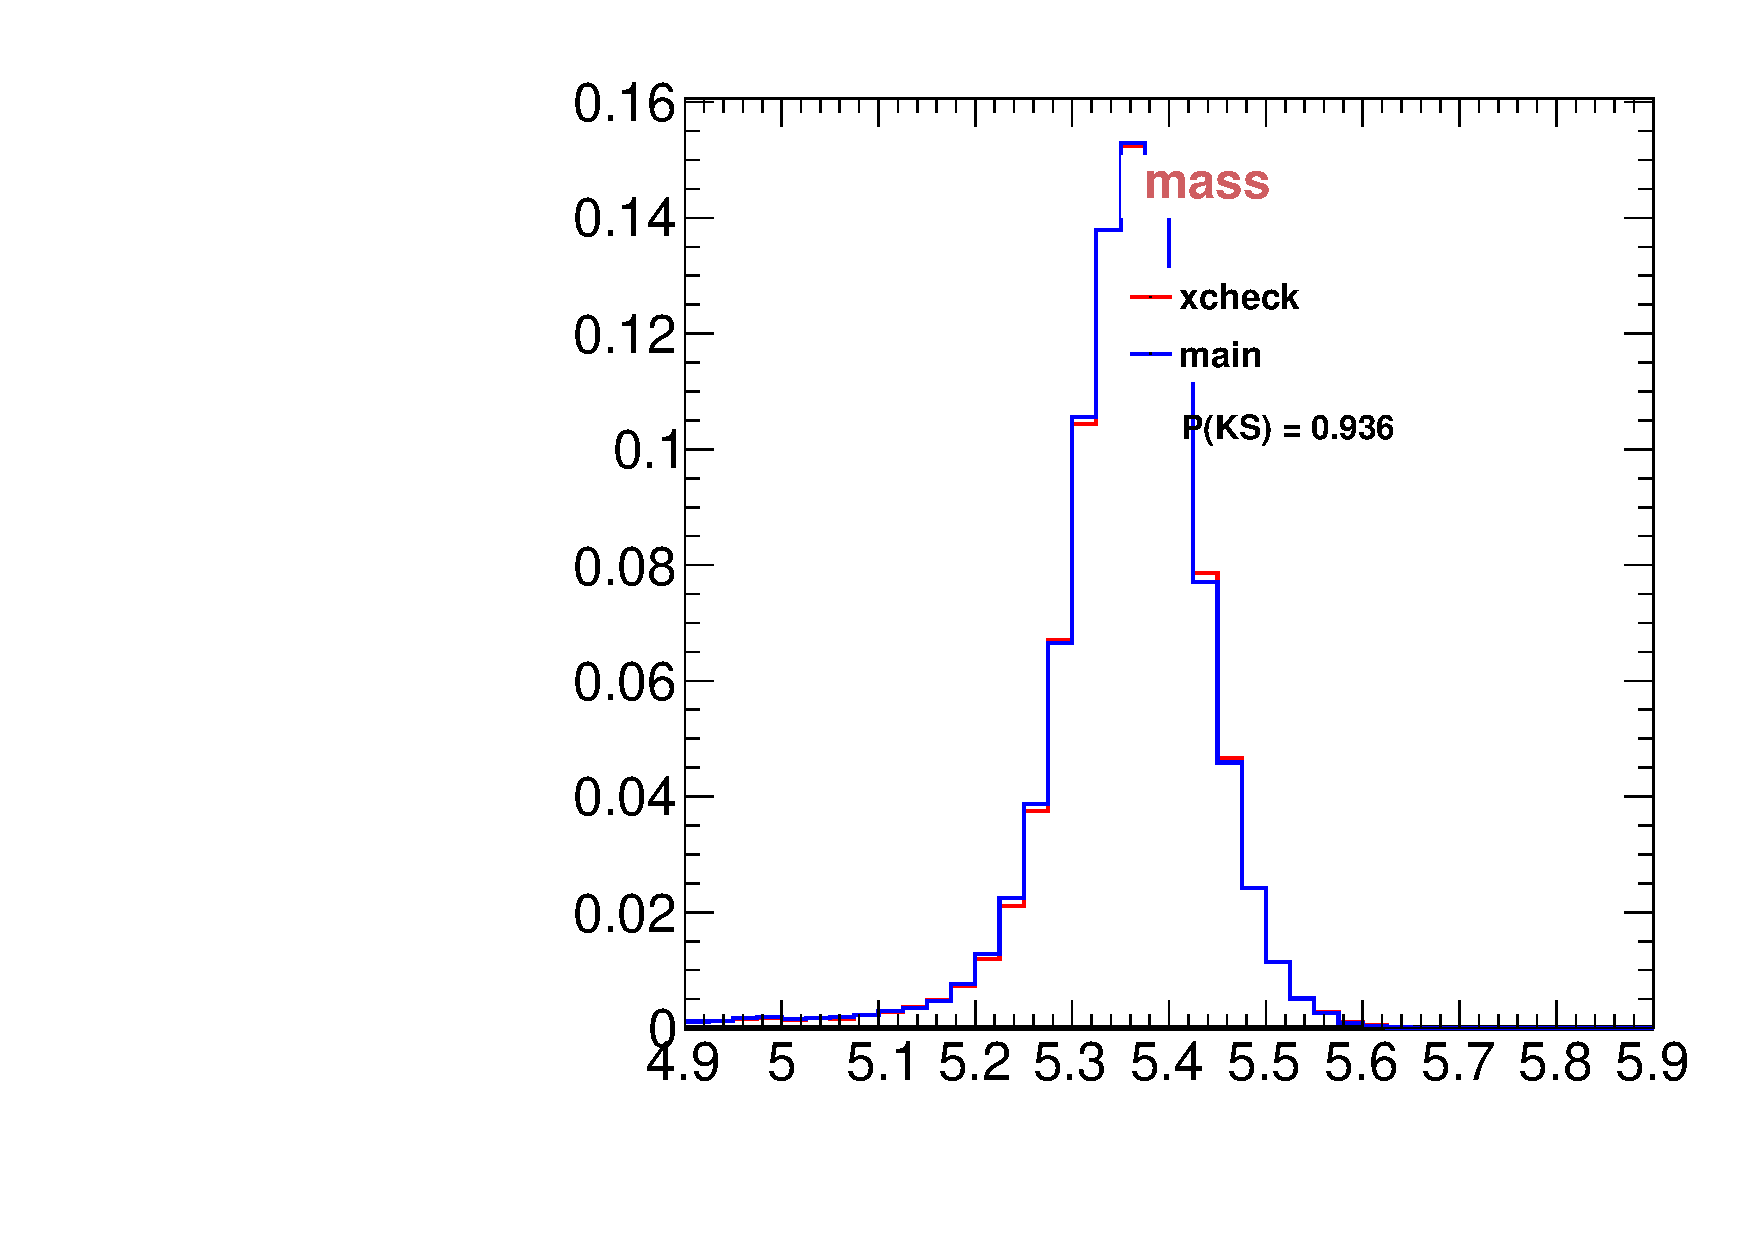
\includegraphics[width=0.3\textwidth]{Figures/VariablesComparison/MC_endcaps_figs/m}
  %\label{fig:MC_endcaps_m}
  \includegraphics[width=0.3\textwidth]{Figures/VariablesComparison/MC_endcaps_figs/m1pt}
  %\label{fig:MC_endcaps_m1pt}
  \includegraphics[width=0.3\textwidth]{Figures/VariablesComparison/MC_endcaps_figs/m2pt}
  %\label{fig:MC_endcaps_m2pt}
  \includegraphics[width=0.3\textwidth]{Figures/VariablesComparison/MC_endcaps_figs/maxdoca}
  %\label{fig:MC_endcaps_maxdoca}
  \includegraphics[width=0.3\textwidth]{Figures/VariablesComparison/MC_endcaps_figs/pt}
  %\label{fig:MC_endcaps_pt}
  \includegraphics[width=0.3\textwidth]{Figures/VariablesComparison/MC_endcaps_figs/pvip}
  %\label{fig:MC_endcaps_pvip}
  \includegraphics[width=0.3\textwidth]{Figures/VariablesComparison/MC_endcaps_figs/pvips}
  %\label{fig:MC_endcaps_pvips}
  \includegraphics[width=0.3\textwidth]{Figures/VariablesComparison/MC_endcaps_figs/pvw8}
  %\label{fig:MC_endcaps_pvw8}
  \includegraphics[width=0.3\textwidth]{Figures/VariablesComparison/MC_endcaps_figs/KS}
  %\label{fig:MC_endcaps_KS}
  \caption{Variable comparisons between the main analysis and the cross-check analysis. Part II: MC endcaps.}
  \label{fig:MC_endcaps_figs}
\end{figure}


\begin{figure}
  \centering
  \includegraphics[width=0.3\textwidth]{Figures/VariablesComparison/Data_barrel_figs/closetrk}
  %\label{fig:Data_barrel_closetrk}
  \includegraphics[width=0.3\textwidth]{Figures/VariablesComparison/Data_barrel_figs/cosa}
  %\label{fig:Data_barrel_cosa}
  \includegraphics[width=0.3\textwidth]{Figures/VariablesComparison/Data_barrel_figs/docatrk}
  %\label{fig:Data_barrel_docatrk}
  \includegraphics[width=0.3\textwidth]{Figures/VariablesComparison/Data_barrel_figs/fl3d}
  %\label{fig:Data_barrel_fl3d}
  \includegraphics[width=0.3\textwidth]{Figures/VariablesComparison/Data_barrel_figs/fls3d}
  %\label{fig:Data_barrel_fls3d}
  \includegraphics[width=0.3\textwidth]{Figures/VariablesComparison/Data_barrel_figs/iso}
  %\label{fig:Data_barrel_iso}
  \includegraphics[width=0.3\textwidth]{Figures/VariablesComparison/Data_barrel_figs/m}
  %\label{fig:Data_barrel_m}
  \includegraphics[width=0.3\textwidth]{Figures/VariablesComparison/Data_barrel_figs/m1pt}
  %\label{fig:Data_barrel_m1pt}
  \includegraphics[width=0.3\textwidth]{Figures/VariablesComparison/Data_barrel_figs/m2pt}
  %\label{fig:Data_barrel_m2pt}
  \includegraphics[width=0.3\textwidth]{Figures/VariablesComparison/Data_barrel_figs/maxdoca}
  %\label{fig:Data_barrel_maxdoca}
  \includegraphics[width=0.3\textwidth]{Figures/VariablesComparison/Data_barrel_figs/pt}
  %\label{fig:Data_barrel_pt}
  \includegraphics[width=0.3\textwidth]{Figures/VariablesComparison/Data_barrel_figs/pvip}
  %\label{fig:Data_barrel_pvip}
  \includegraphics[width=0.3\textwidth]{Figures/VariablesComparison/Data_barrel_figs/pvips}
  %\label{fig:Data_barrel_pvips}
  \includegraphics[width=0.3\textwidth]{Figures/VariablesComparison/Data_barrel_figs/pvw8}
  %\label{fig:Data_barrel_pvw8}
  \includegraphics[width=0.3\textwidth]{Figures/VariablesComparison/Data_barrel_figs/KS}
  %\label{fig:Data_barrel_KS}
  \caption{Variable comparisons between the main analysis and the cross-check analysis. Part III: Data barrel.}
  \label{fig:Data_barrel_figs}
\end{figure}


\begin{figure}
  \centering
  \includegraphics[width=0.3\textwidth]{Figures/VariablesComparison/Data_endcaps_figs/closetrk}
  %\label{fig:Data_endcaps_closetrk}
  \includegraphics[width=0.3\textwidth]{Figures/VariablesComparison/Data_endcaps_figs/cosa}
  %\label{fig:Data_endcaps_cosa}
  \includegraphics[width=0.3\textwidth]{Figures/VariablesComparison/Data_endcaps_figs/docatrk}
  %\label{fig:Data_endcaps_docatrk}
  \includegraphics[width=0.3\textwidth]{Figures/VariablesComparison/Data_endcaps_figs/fl3d}
  %\label{fig:Data_endcaps_fl3d}
  \includegraphics[width=0.3\textwidth]{Figures/VariablesComparison/Data_endcaps_figs/fls3d}
  %\label{fig:Data_endcaps_fls3d}
  \includegraphics[width=0.3\textwidth]{Figures/VariablesComparison/Data_endcaps_figs/iso}
  %\label{fig:Data_endcaps_iso}
  \includegraphics[width=0.3\textwidth]{Figures/VariablesComparison/Data_endcaps_figs/m}
  %\label{fig:Data_endcaps_m}
  \includegraphics[width=0.3\textwidth]{Figures/VariablesComparison/Data_endcaps_figs/m1pt}
  %\label{fig:Data_endcaps_m1pt}
  \includegraphics[width=0.3\textwidth]{Figures/VariablesComparison/Data_endcaps_figs/m2pt}
  %\label{fig:Data_endcaps_m2pt}
  \includegraphics[width=0.3\textwidth]{Figures/VariablesComparison/Data_endcaps_figs/maxdoca}
  %\label{fig:Data_endcaps_maxdoca}
  \includegraphics[width=0.3\textwidth]{Figures/VariablesComparison/Data_endcaps_figs/pt}
  %\label{fig:Data_endcaps_pt}
  \includegraphics[width=0.3\textwidth]{Figures/VariablesComparison/Data_endcaps_figs/pvip}
  %\label{fig:Data_endcaps_pvip}
  \includegraphics[width=0.3\textwidth]{Figures/VariablesComparison/Data_endcaps_figs/pvips}
  %\label{fig:Data_endcaps_pvips}
  \includegraphics[width=0.3\textwidth]{Figures/VariablesComparison/Data_endcaps_figs/pvw8}
  %\label{fig:Data_endcaps_pvw8}
  \includegraphics[width=0.3\textwidth]{Figures/VariablesComparison/Data_endcaps_figs/KS}
  %\label{fig:Data_endcaps_KS}
  \caption{Variable comparisons between the main analysis and the cross-check analysis. Part IV: Data endcaps.}
  \label{fig:Data_endcaps_figs}
\end{figure}



\begin{sidewaysfigure}
        \centering
        \begin{subfigure}[b]{0.2\textwidth}
                \centering
                \includegraphics[width=\textwidth]{Figures/VariablesComparison/MC_barrel_figs_3h/ntrk}
                \label{fig:MC_barrel_ntrk_3h}
        \end{subfigure}
        \begin{subfigure}[b]{0.2\textwidth}
                \centering
                \includegraphics[width=\textwidth]{Figures/VariablesComparison/MC_barrel_figs_3h/cosAlpha3D}
                \label{fig:MC_barrel_cosAlpha3D_3h}
        \end{subfigure}
        \begin{subfigure}[b]{0.2\textwidth}
                \centering
                \includegraphics[width=\textwidth]{Figures/VariablesComparison/MC_barrel_figs_3h/minDca}
                \label{fig:MC_barrel_minDca_3h}
        \end{subfigure}
        \begin{subfigure}[b]{0.2\textwidth}
                \centering
                \includegraphics[width=\textwidth]{Figures/VariablesComparison/MC_barrel_figs_3h/l3d}
                \label{fig:MC_barrel_l3d_3h}
        \end{subfigure}
        \begin{subfigure}[b]{0.2\textwidth}
                \centering
                \includegraphics[width=\textwidth]{Figures/VariablesComparison/MC_barrel_figs_3h/l3dsig}
                \label{fig:MC_barrel_l3dsig_3h}
        \end{subfigure}
        \begin{subfigure}[b]{0.2\textwidth}
                \centering
                \includegraphics[width=\textwidth]{Figures/VariablesComparison/MC_barrel_figs_3h/isolation}
                \label{fig:MC_barrel_isolation_3h}
        \end{subfigure}
        \begin{subfigure}[b]{0.2\textwidth}
                \centering
                \includegraphics[width=\textwidth]{Figures/VariablesComparison/MC_barrel_figs_3h/mass}
                \label{fig:MC_barrel_mass_3h}
        \end{subfigure}
        \begin{subfigure}[b]{0.2\textwidth}
                \centering
                \includegraphics[width=\textwidth]{Figures/VariablesComparison/MC_barrel_figs_3h/mu1_pt}
                \label{fig:MC_barrel_mu1_pt_3h}
        \end{subfigure}
        \begin{subfigure}[b]{0.2\textwidth}
                \centering
                \includegraphics[width=\textwidth]{Figures/VariablesComparison/MC_barrel_figs_3h/mu2_pt}
                \label{fig:MC_barrel_mu2_pt_3h}
        \end{subfigure}
        \begin{subfigure}[b]{0.2\textwidth}
                \centering
                \includegraphics[width=\textwidth]{Figures/VariablesComparison/MC_barrel_figs_3h/dca}
                \label{fig:MC_barrel_dca_3h}
        \end{subfigure}
        \begin{subfigure}[b]{0.2\textwidth}
                \centering
                \includegraphics[width=\textwidth]{Figures/VariablesComparison/MC_barrel_figs_3h/pt}
                \label{fig:MC_barrel_pt_3h}
        \end{subfigure}
        \begin{subfigure}[b]{0.2\textwidth}
                \centering
                \includegraphics[width=\textwidth]{Figures/VariablesComparison/MC_barrel_figs_3h/delta3d}
                \label{fig:MC_barrel_delta3d_3h}
        \end{subfigure}
        \begin{subfigure}[b]{0.2\textwidth}
                \centering
                \includegraphics[width=\textwidth]{Figures/VariablesComparison/MC_barrel_figs_3h/delta3dErr}
                \label{fig:MC_barrel_delta3d/delta3dErr_3h}
        \end{subfigure}
        \begin{subfigure}[b]{0.2\textwidth}
                \centering
                \includegraphics[width=\textwidth]{Figures/VariablesComparison/MC_barrel_figs_3h/pvw8}
                \label{fig:MC_barrel_pvw8_3h}
        \end{subfigure}
        \begin{subfigure}[b]{0.2\textwidth}
                \centering
                \includegraphics[width=\textwidth]{Figures/VariablesComparison/MC_barrel_figs_3h/KS}
                \label{fig:MC_barrel_KS_3h}
        \end{subfigure}
        \caption{Overlay of BDT training variable distributions in Signal MC for events of the three subsets in the barrel. The plot on the bottom right summarizes all KS probablities.}
        \label{fig:MC_barrel_figs_3h}
\end{sidewaysfigure}


\begin{sidewaysfigure}
        \centering
        \begin{subfigure}[b]{0.2\textwidth}
                \centering
                \includegraphics[width=\textwidth]{Figures/VariablesComparison/MC_endcaps_figs_3h/ntrk}
                \label{fig:MC_endcaps_ntrk_3h}
        \end{subfigure}
        \begin{subfigure}[b]{0.2\textwidth}
                \centering
                \includegraphics[width=\textwidth]{Figures/VariablesComparison/MC_endcaps_figs_3h/cosAlpha3D}
                \label{fig:MC_endcaps_cosAlpha3D_3h}
        \end{subfigure}
        \begin{subfigure}[b]{0.2\textwidth}
                \centering
                \includegraphics[width=\textwidth]{Figures/VariablesComparison/MC_endcaps_figs_3h/minDca}
                \label{fig:MC_endcaps_minDca_3h}
        \end{subfigure}
        \begin{subfigure}[b]{0.2\textwidth}
                \centering
                \includegraphics[width=\textwidth]{Figures/VariablesComparison/MC_endcaps_figs_3h/l3d}
                \label{fig:MC_endcaps_l3d_3h}
        \end{subfigure}
        \begin{subfigure}[b]{0.2\textwidth}
                \centering
                \includegraphics[width=\textwidth]{Figures/VariablesComparison/MC_endcaps_figs_3h/l3dsig}
                \label{fig:MC_endcaps_l3dsig_3h}
        \end{subfigure}
        \begin{subfigure}[b]{0.2\textwidth}
                \centering
                \includegraphics[width=\textwidth]{Figures/VariablesComparison/MC_endcaps_figs_3h/isolation}
                \label{fig:MC_endcaps_isolation_3h}
        \end{subfigure}
        \begin{subfigure}[b]{0.2\textwidth}
                \centering
                \includegraphics[width=\textwidth]{Figures/VariablesComparison/MC_endcaps_figs_3h/mass}
                \label{fig:MC_endcaps_mass_3h}
        \end{subfigure}
        \begin{subfigure}[b]{0.2\textwidth}
                \centering
                \includegraphics[width=\textwidth]{Figures/VariablesComparison/MC_endcaps_figs_3h/mu1_pt}
                \label{fig:MC_endcaps_mu1_pt_3h}
        \end{subfigure}
        \begin{subfigure}[b]{0.2\textwidth}
                \centering
                \includegraphics[width=\textwidth]{Figures/VariablesComparison/MC_endcaps_figs_3h/mu2_pt}
                \label{fig:MC_endcaps_mu2_pt_3h}
        \end{subfigure}
        \begin{subfigure}[b]{0.2\textwidth}
                \centering
                \includegraphics[width=\textwidth]{Figures/VariablesComparison/MC_endcaps_figs_3h/dca}
                \label{fig:MC_endcaps_dca_3h}
        \end{subfigure}
        \begin{subfigure}[b]{0.2\textwidth}
                \centering
                \includegraphics[width=\textwidth]{Figures/VariablesComparison/MC_endcaps_figs_3h/pt}
                \label{fig:MC_endcaps_pt_3h}
        \end{subfigure}
        \begin{subfigure}[b]{0.2\textwidth}
                \centering
                \includegraphics[width=\textwidth]{Figures/VariablesComparison/MC_endcaps_figs_3h/delta3d}
                \label{fig:MC_endcaps_delta3d_3h}
        \end{subfigure}
        \begin{subfigure}[b]{0.2\textwidth}
                \centering
                \includegraphics[width=\textwidth]{Figures/VariablesComparison/MC_endcaps_figs_3h/delta3dErr}
                \label{fig:MC_endcaps_delta3d/delta3dErr_3h}
        \end{subfigure}
        \begin{subfigure}[b]{0.2\textwidth}
                \centering
                \includegraphics[width=\textwidth]{Figures/VariablesComparison/MC_endcaps_figs_3h/pvw8}
                \label{fig:MC_endcaps_pvw8_3h}
        \end{subfigure}
        \begin{subfigure}[b]{0.2\textwidth}
                \centering
                \includegraphics[width=\textwidth]{Figures/VariablesComparison/MC_endcaps_figs_3h/KS}
                \label{fig:MC_endcaps_KS_3h}
        \end{subfigure}
        \caption{Overlay of BDT training variable distributions in Signal MC for events of the three subsets in the endcap. The plot on the bottom right summarizes all KS probablities.}
        \label{fig:MC_endcaps_figs_3h}
\end{sidewaysfigure}


\begin{sidewaysfigure}
        \centering
        \begin{subfigure}[b]{0.2\textwidth}
                \centering
                \includegraphics[width=\textwidth]{Figures/VariablesComparison/Data_barrel_figs_3h/ntrk}
                \label{fig:Data_barrel_ntrk_3h}
        \end{subfigure}
        \begin{subfigure}[b]{0.2\textwidth}
                \centering
                \includegraphics[width=\textwidth]{Figures/VariablesComparison/Data_barrel_figs_3h/cosAlpha3D}
                \label{fig:Data_barrel_cosAlpha3D_3h}
        \end{subfigure}
        \begin{subfigure}[b]{0.2\textwidth}
                \centering
                \includegraphics[width=\textwidth]{Figures/VariablesComparison/Data_barrel_figs_3h/minDca}
                \label{fig:Data_barrel_minDca_3h}
        \end{subfigure}
        \begin{subfigure}[b]{0.2\textwidth}
                \centering
                \includegraphics[width=\textwidth]{Figures/VariablesComparison/Data_barrel_figs_3h/l3d}
                \label{fig:Data_barrel_l3d_3h}
        \end{subfigure}
        \begin{subfigure}[b]{0.2\textwidth}
                \centering
                \includegraphics[width=\textwidth]{Figures/VariablesComparison/Data_barrel_figs_3h/l3dsig}
                \label{fig:Data_barrel_l3dsig_3h}
        \end{subfigure}
        \begin{subfigure}[b]{0.2\textwidth}
                \centering
                \includegraphics[width=\textwidth]{Figures/VariablesComparison/Data_barrel_figs_3h/isolation}
                \label{fig:Data_barrel_isolation_3h}
        \end{subfigure}
        \begin{subfigure}[b]{0.2\textwidth}
                \centering
                \includegraphics[width=\textwidth]{Figures/VariablesComparison/Data_barrel_figs_3h/mass}
                \label{fig:Data_barrel_mass_3h}
        \end{subfigure}
        \begin{subfigure}[b]{0.2\textwidth}
                \centering
                \includegraphics[width=\textwidth]{Figures/VariablesComparison/Data_barrel_figs_3h/mu1_pt}
                \label{fig:Data_barrel_mu1_pt_3h}
        \end{subfigure}
        \begin{subfigure}[b]{0.2\textwidth}
                \centering
                \includegraphics[width=\textwidth]{Figures/VariablesComparison/Data_barrel_figs_3h/mu2_pt}
                \label{fig:Data_barrel_mu2_pt_3h}
        \end{subfigure}
        \begin{subfigure}[b]{0.2\textwidth}
                \centering
                \includegraphics[width=\textwidth]{Figures/VariablesComparison/Data_barrel_figs_3h/dca}
                \label{fig:Data_barrel_dca_3h}
        \end{subfigure}
        \begin{subfigure}[b]{0.2\textwidth}
                \centering
                \includegraphics[width=\textwidth]{Figures/VariablesComparison/Data_barrel_figs_3h/pt}
                \label{fig:Data_barrel_pt_3h}
        \end{subfigure}
        \begin{subfigure}[b]{0.2\textwidth}
                \centering
                \includegraphics[width=\textwidth]{Figures/VariablesComparison/Data_barrel_figs_3h/delta3d}
                \label{fig:Data_barrel_delta3d_3h}
        \end{subfigure}
        \begin{subfigure}[b]{0.2\textwidth}
                \centering
                \includegraphics[width=\textwidth]{Figures/VariablesComparison/Data_barrel_figs_3h/delta3dErr}
                \label{fig:Data_barrel_delta3d/delta3dErr_3h}
        \end{subfigure}
        \begin{subfigure}[b]{0.2\textwidth}
                \centering
                \includegraphics[width=\textwidth]{Figures/VariablesComparison/Data_barrel_figs_3h/pvw8}
                \label{fig:Data_barrel_pvw8_3h}
        \end{subfigure}
        \begin{subfigure}[b]{0.2\textwidth}
                \centering
                \includegraphics[width=\textwidth]{Figures/VariablesComparison/Data_barrel_figs_3h/KS}
                \label{fig:Data_barrel_KS_3h}
        \end{subfigure}
        \caption{Overlay of BDT training variable distributions in data sideband background for events of the three subsets in the barrel. The plot on the bottom right summarizes all KS probablities.}
        \label{fig:Data_barrel_figs_3h}
\end{sidewaysfigure}


\begin{sidewaysfigure}
        \centering
        \begin{subfigure}[b]{0.2\textwidth}
                \centering
                \includegraphics[width=\textwidth]{Figures/VariablesComparison/Data_endcaps_figs_3h/ntrk}
                \label{fig:Data_endcaps_ntrk_3h}
        \end{subfigure}
        \begin{subfigure}[b]{0.2\textwidth}
                \centering
                \includegraphics[width=\textwidth]{Figures/VariablesComparison/Data_endcaps_figs_3h/cosAlpha3D}
                \label{fig:Data_endcaps_cosAlpha3D_3h}
        \end{subfigure}
        \begin{subfigure}[b]{0.2\textwidth}
                \centering
                \includegraphics[width=\textwidth]{Figures/VariablesComparison/Data_endcaps_figs_3h/minDca}
                \label{fig:Data_endcaps_minDca_3h}
        \end{subfigure}
        \begin{subfigure}[b]{0.2\textwidth}
                \centering
                \includegraphics[width=\textwidth]{Figures/VariablesComparison/Data_endcaps_figs_3h/l3d}
                \label{fig:Data_endcaps_l3d_3h}
        \end{subfigure}
        \begin{subfigure}[b]{0.2\textwidth}
                \centering
                \includegraphics[width=\textwidth]{Figures/VariablesComparison/Data_endcaps_figs_3h/l3dsig}
                \label{fig:Data_endcaps_l3dsig_3h}
        \end{subfigure}
        \begin{subfigure}[b]{0.2\textwidth}
                \centering
                \includegraphics[width=\textwidth]{Figures/VariablesComparison/Data_endcaps_figs_3h/isolation}
                \label{fig:Data_endcaps_isolation_3h}
        \end{subfigure}
        \begin{subfigure}[b]{0.2\textwidth}
                \centering
                \includegraphics[width=\textwidth]{Figures/VariablesComparison/Data_endcaps_figs_3h/mass}
                \label{fig:Data_endcaps_mass_3h}
        \end{subfigure}
        \begin{subfigure}[b]{0.2\textwidth}
                \centering
                \includegraphics[width=\textwidth]{Figures/VariablesComparison/Data_endcaps_figs_3h/mu1_pt}
                \label{fig:Data_endcaps_mu1_pt_3h}
        \end{subfigure}
        \begin{subfigure}[b]{0.2\textwidth}
                \centering
                \includegraphics[width=\textwidth]{Figures/VariablesComparison/Data_endcaps_figs_3h/mu2_pt}
                \label{fig:Data_endcaps_mu2_pt_3h}
        \end{subfigure}
        \begin{subfigure}[b]{0.2\textwidth}
                \centering
                \includegraphics[width=\textwidth]{Figures/VariablesComparison/Data_endcaps_figs_3h/dca}
                \label{fig:Data_endcaps_dca_3h}
        \end{subfigure}
        \begin{subfigure}[b]{0.2\textwidth}
                \centering
                \includegraphics[width=\textwidth]{Figures/VariablesComparison/Data_endcaps_figs_3h/pt}
                \label{fig:Data_endcaps_pt_3h}
        \end{subfigure}
        \begin{subfigure}[b]{0.2\textwidth}
                \centering
                \includegraphics[width=\textwidth]{Figures/VariablesComparison/Data_endcaps_figs_3h/delta3d}
                \label{fig:Data_endcaps_delta3d_3h}
        \end{subfigure}
        \begin{subfigure}[b]{0.2\textwidth}
                \centering
                \includegraphics[width=\textwidth]{Figures/VariablesComparison/Data_endcaps_figs_3h/delta3dErr}
                \label{fig:Data_endcaps_delta3d/delta3dErr_3h}
        \end{subfigure}
        \begin{subfigure}[b]{0.2\textwidth}
                \centering
                \includegraphics[width=\textwidth]{Figures/VariablesComparison/Data_endcaps_figs_3h/pvw8}
                \label{fig:Data_endcaps_pvw8_3h}
        \end{subfigure}
        \begin{subfigure}[b]{0.2\textwidth}
                \centering
                \includegraphics[width=\textwidth]{Figures/VariablesComparison/Data_endcaps_figs_3h/KS}
                \label{fig:Data_endcaps_KS_3h}
        \end{subfigure}
        \caption{Overlay of BDT training variable distributions in data sideband background for events of the three subsets in the endcap. The plot on the bottom right summarizes all KS probablities.}
        \label{fig:Data_endcaps_figs_3h}
\end{sidewaysfigure}




\section{Boosted Decision Tree}

The inclusive samples are split in three different subsamples according to the rule $index = eventNumber\%3$.
These samples are then used as follows:
\begin{itemize}
\item events of type 0: analyzed by BDT0, trained on type-1 events, tested on type-2 events
\item events of type 1: analyzed by BDT1, trained on type-2 events, tested on type-0 events
\item events of type 2: analyzed by BDT2, trained on type-0 events, tested on type-1 events
\end{itemize}
for the training and testing.

Tables \ref{tab:datasetsbarrelBDT} and \ref{tab:datasetsendcapsBDT} show the ranking of variables before
the BDT training.
\input{Tables/ranking_barrel_BDT.txt}
\input{Tables/ranking_endcaps_BDT.txt}

Tables \ref{tab:numEvents} shows the number of candidates in each of the subsamples. The events are after
all preselections including muon-id (tight muon).
\input{Tables/numCandidates.txt}

Figure \ref{fig:BDTControlPlots} shows control plots for the BDT training.

\begin{figure}
  \centering
  \includegraphics[width=0.45\textwidth]{Figures/BDTControlPlots_barrel}
  \includegraphics[width=0.45\textwidth]{Figures/BDTControlPlots_endcaps}
  \caption{TMVA BDT charaterization plots for the barrel (left) and the endcap (right). Shown versus the tree number is the boost weight (top) and the event misclassification rate (middle), and the number of nodes before pruning (bottom).}
  \label{fig:BDTControlPlots}
\end{figure}



\clearpage
\section{Cut and count analysis}
\subsection{optimization and blinded results}
\subsection{unblind}

\section{BDT analysis}
\subsection{training and overtraining}
\subsection{blinded results}
\subsection{unblind}


\section{BDT analysis}

Figures \ref{fig:massOptimalCut} show the optimal value of the BDT cut for the estimated numbers of signal and background
events.

Figures \ref{fig:massPlotBlinded} show the blinded invariant mass distribution after applying the BDT selection.

\begin{figure}
  \centering
  \includegraphics[width=0.45\textwidth]{Figures/mvaeffs_BDT_barrel.pdf}
  \includegraphics[width=0.45\textwidth]{Figures/mvaeffs_BDT_endcaps.pdf}
  \caption{Optimal BDT cut value for barrel (left) and endcaps (right).}
  \label{fig:massOptimalCut}
\end{figure}

\begin{figure}
  \centering
  \includegraphics[width=0.45\textwidth]{Figures/BarrelMassPlot.pdf}
  \includegraphics[width=0.45\textwidth]{Figures/EndcapsMassPlot.pdf}
  \caption{Blinded invariant mass distribution for all candidates passing the BDT selection for barrel (left) and endcaps (right).}
  \label{fig:massPlotBlinded}
\end{figure}

Figures \ref{fig:massPlotUnblinded} shows the unblinded invariant mass distribution after applying the BDT selection.

\begin{figure}
  \centering
  \includegraphics[width=0.45\textwidth]{Figures/BarrelMassPlotUnblinded.pdf}
  \includegraphics[width=0.45\textwidth]{Figures/EndcapsMassPlotUnblinded.pdf}
  \caption{Unblinded invariant mass distribution for all candidates passing the BDT selection for barrel (left) and endcaps (right).}
  \label{fig:massPlotUnblinded}
\end{figure}


Figures

\begin{figure}
  \centering
  \includegraphics[width=0.3\textwidth]{Figures/AfterBDTCut_pt_Barrel.pdf}
  \includegraphics[width=0.3\textwidth]{Figures/AfterBDTCut_eta_Barrel.pdf}
  \includegraphics[width=0.3\textwidth]{Figures/AfterBDTCut_fls3d_Barrel.pdf}
  \includegraphics[width=0.3\textwidth]{Figures/AfterBDTCut_alpha_Barrel.pdf}
  \includegraphics[width=0.3\textwidth]{Figures/AfterBDTCut_maxdoca_Barrel.pdf}
  \includegraphics[width=0.3\textwidth]{Figures/AfterBDTCut_pvip_Barrel.pdf}
  \includegraphics[width=0.3\textwidth]{Figures/AfterBDTCut_pvips_Barrel.pdf}
  \includegraphics[width=0.3\textwidth]{Figures/AfterBDTCut_iso_Barrel.pdf}
  \includegraphics[width=0.3\textwidth]{Figures/AfterBDTCut_docatrk_Barrel.pdf}
  \includegraphics[width=0.3\textwidth]{Figures/AfterBDTCut_closetrk_Barrel.pdf}
  \includegraphics[width=0.3\textwidth]{Figures/AfterBDTCut_chi2dof_Barrel.pdf}
  \caption{Variable distributions for the barrel after BDT cuts on blinded data.}
  \label{fig:massPlotUnblinded}
\end{figure}

\begin{figure}
  \centering
  \includegraphics[width=0.3\textwidth]{Figures/AfterBDTCut_pt_Endcaps.pdf}
  \includegraphics[width=0.3\textwidth]{Figures/AfterBDTCut_eta_Endcaps.pdf}
  \includegraphics[width=0.3\textwidth]{Figures/AfterBDTCut_fls3d_Endcaps.pdf}
  \includegraphics[width=0.3\textwidth]{Figures/AfterBDTCut_alpha_Endcaps.pdf}
  \includegraphics[width=0.3\textwidth]{Figures/AfterBDTCut_maxdoca_Endcaps.pdf}
  \includegraphics[width=0.3\textwidth]{Figures/AfterBDTCut_pvip_Endcaps.pdf}
  \includegraphics[width=0.3\textwidth]{Figures/AfterBDTCut_pvips_Endcaps.pdf}
  \includegraphics[width=0.3\textwidth]{Figures/AfterBDTCut_iso_Endcaps.pdf}
  \includegraphics[width=0.3\textwidth]{Figures/AfterBDTCut_docatrk_Endcaps.pdf}
  \includegraphics[width=0.3\textwidth]{Figures/AfterBDTCut_closetrk_Endcaps.pdf}
  \includegraphics[width=0.3\textwidth]{Figures/AfterBDTCut_chi2dof_Endcaps.pdf}
  \caption{Variable distributions for the endcaps after BDT cuts on blinded data.}
  \label{fig:massPlotUnblinded}
\end{figure}

\begin{figure}
  \centering
  \includegraphics[width=0.3\textwidth]{Figures/AfterBDTCut_pt_BarrelUnblinded.pdf}
  \includegraphics[width=0.3\textwidth]{Figures/AfterBDTCut_eta_BarrelUnblinded.pdf}
  \includegraphics[width=0.3\textwidth]{Figures/AfterBDTCut_fls3d_BarrelUnblinded.pdf}
  \includegraphics[width=0.3\textwidth]{Figures/AfterBDTCut_alpha_BarrelUnblinded.pdf}
  \includegraphics[width=0.3\textwidth]{Figures/AfterBDTCut_maxdoca_BarrelUnblinded.pdf}
  \includegraphics[width=0.3\textwidth]{Figures/AfterBDTCut_pvip_BarrelUnblinded.pdf}
  \includegraphics[width=0.3\textwidth]{Figures/AfterBDTCut_pvips_BarrelUnblinded.pdf}
  \includegraphics[width=0.3\textwidth]{Figures/AfterBDTCut_iso_BarrelUnblinded.pdf}
  \includegraphics[width=0.3\textwidth]{Figures/AfterBDTCut_docatrk_BarrelUnblinded.pdf}
  \includegraphics[width=0.3\textwidth]{Figures/AfterBDTCut_closetrk_BarrelUnblinded.pdf}
  \includegraphics[width=0.3\textwidth]{Figures/AfterBDTCut_chi2dof_BarrelUnblinded.pdf}
  \caption{Variable distributions for the barrel after BDT cuts on unblinded data.}
  \label{fig:massPlotUnblinded}
\end{figure}

\begin{figure}
  \centering
  \includegraphics[width=0.3\textwidth]{Figures/AfterBDTCut_pt_EndcapsUnblinded.pdf}
  \includegraphics[width=0.3\textwidth]{Figures/AfterBDTCut_eta_EndcapsUnblinded.pdf}
  \includegraphics[width=0.3\textwidth]{Figures/AfterBDTCut_fls3d_EndcapsUnblinded.pdf}
  \includegraphics[width=0.3\textwidth]{Figures/AfterBDTCut_alpha_EndcapsUnblinded.pdf}
  \includegraphics[width=0.3\textwidth]{Figures/AfterBDTCut_maxdoca_EndcapsUnblinded.pdf}
  \includegraphics[width=0.3\textwidth]{Figures/AfterBDTCut_pvip_EndcapsUnblinded.pdf}
  \includegraphics[width=0.3\textwidth]{Figures/AfterBDTCut_pvips_EndcapsUnblinded.pdf}
  \includegraphics[width=0.3\textwidth]{Figures/AfterBDTCut_iso_EndcapsUnblinded.pdf}
  \includegraphics[width=0.3\textwidth]{Figures/AfterBDTCut_docatrk_EndcapsUnblinded.pdf}
  \includegraphics[width=0.3\textwidth]{Figures/AfterBDTCut_closetrk_EndcapsUnblinded.pdf}
  \includegraphics[width=0.3\textwidth]{Figures/AfterBDTCut_chi2dof_EndcapsUnblinded.pdf}
  \caption{Variable distributions for the endcaps after BDT cuts on unblinded data.}
  \label{fig:massPlotUnblinded}
\end{figure}


\begin{figure}
  \centering
  \includegraphics[width=0.45\textwidth]{Figures/bdt/BDT_barrel_roc}
  \includegraphics[width=0.45\textwidth]{Figures/bdt/BDT_barrel_eff} \\
  \includegraphics[width=0.45\textwidth]{Figures/bdt/BDT_barrel_mass}
  \includegraphics[width=0.45\textwidth]{Figures/bdt/BDT_barrel_mass_unblind}
\caption{BDT barrel}
\end{figure}

\begin{figure}
  \centering
  \includegraphics[width=0.45\textwidth]{Figures/mlp/MLP_barrel_roc}
  \includegraphics[width=0.45\textwidth]{Figures/mlp/MLP_barrel_eff} \\
  \includegraphics[width=0.45\textwidth]{Figures/mlp/MLP_barrel_mass}
  \includegraphics[width=0.45\textwidth]{Figures/mlp/MLP_barrel_mass_unblind}
\caption{MLP barrel}
\end{figure}


%%%
\begin{figure}
  \centering
  \includegraphics[width=0.45\textwidth]{Figures/bdt/BDT_endcaps_roc}
  \includegraphics[width=0.45\textwidth]{Figures/bdt/BDT_endcaps_eff} \\
  \includegraphics[width=0.45\textwidth]{Figures/bdt/BDT_endcaps_mass}
  \includegraphics[width=0.45\textwidth]{Figures/bdt/BDT_endcaps_mass_unblind}
\caption{BDT endcaps}
\end{figure}

\begin{figure}
  \centering
  \includegraphics[width=0.45\textwidth]{Figures/mlp/MLP_endcaps_roc}
  \includegraphics[width=0.45\textwidth]{Figures/mlp/MLP_endcaps_eff} \\
  \includegraphics[width=0.45\textwidth]{Figures/mlp/MLP_endcaps_mass}
  \includegraphics[width=0.45\textwidth]{Figures/mlp/MLP_endcaps_mass_unblind}
\caption{MLP endcaps}
\end{figure}


\section{Normalization channel}
\subsection{datasets}
\subsection{selection}
\subsection{BDT}
\subsection{yields}

\cleardoublepage\addcontentsline{toc}{section}{Part II (full updated analysis)}

\section{Full dataset}
\section{Selection}
\subsection{datasets}
\subsection{muon identification}
\subsection{variable distributions, correlations, ranking}
\subsection{TMVA training}
\subsubsection{MLP}
\subsubsection{BDT}
\subsection{Normalization channel}
\subsubsection{MLP}
\subsubsection{BDT}
\subsection{Limits}


\section{Summary}


\bibliographystyle{plain}
\bibliography{BsMuMuCrossCheckAnalysis}

\end{document}
